\documentclass[paper=a4]{scrartcl}
  
\usepackage[ansinew]{inputenc}
\usepackage[T1]{fontenc}
\usepackage[english]{babel}
\usepackage{graphicx}
\usepackage{caption,subfig} % z.B. [font=scriptsize]
\usepackage[alsoload=binary]{siunitx}
\usepackage[numbers,sort&compress]{natbib}
\usepackage{microtype}
%  \DisableLigatures{encoding = *, family = * }
\usepackage{tikz}
\usepackage{pgfplots}
\usepackage{hyperref}

\newcommand{\imsize}{.5\linewidth}

\newcommand{\footremember}[2]{\footnote{#2}\newcounter{#1}\setcounter{#1}{\value{footnote}}}
\newcommand{\footrecall}[1]{\footnotemark[\value{#1}]} 

\newlength\imagewidth           % needed for scalebars
\newlength\imagescale           % ditto

\title{Distance Transformation of ROIs}
\author{David Haberth�r}

\begin{document}

\maketitle

I've extracted 4 regions of interest with a side length of 256 pixels (\SI{1.48}{\micro\meter\per pixel}, thus a volume of \SI{1.678e7}{px}) for the protocols B, L and T, as shown in figure~\ref{fig:roi3d}. Each of these ROIs has been thresholded using an Otsu-Threshold (see figure~\ref{fig:synchroview}, left), hence no bias has been introduced due to the obvserver\footnote{The threshold has been calculated to be ``52'', for the \SI{8}{\bit}-images}. Using a connected components analysis I've removed small particles inside the airway lumen and subsequently performed a euclidean distance transformation to analyze the ``thickness'' of the airways (see figure~\ref{fig:synchroview}, right).

\renewcommand{\imsize}{\columnwidth}
\begin{figure}[h]%
	\centering
	\pgfmathsetlength{\imagewidth}{\imsize}%
	\pgfmathsetlength{\imagescale}{\imagewidth/1452}%
	\begin{tikzpicture}[x=\imagescale,y=-\imagescale]
		\def\x{897} % scalebar-x at golden ratio of x=1452px
		\def\y{684} % scalebar-y at 90% of height of y=760px
		\node[anchor=north west,inner sep=0pt,outer sep=0pt] at (0,0)
	     {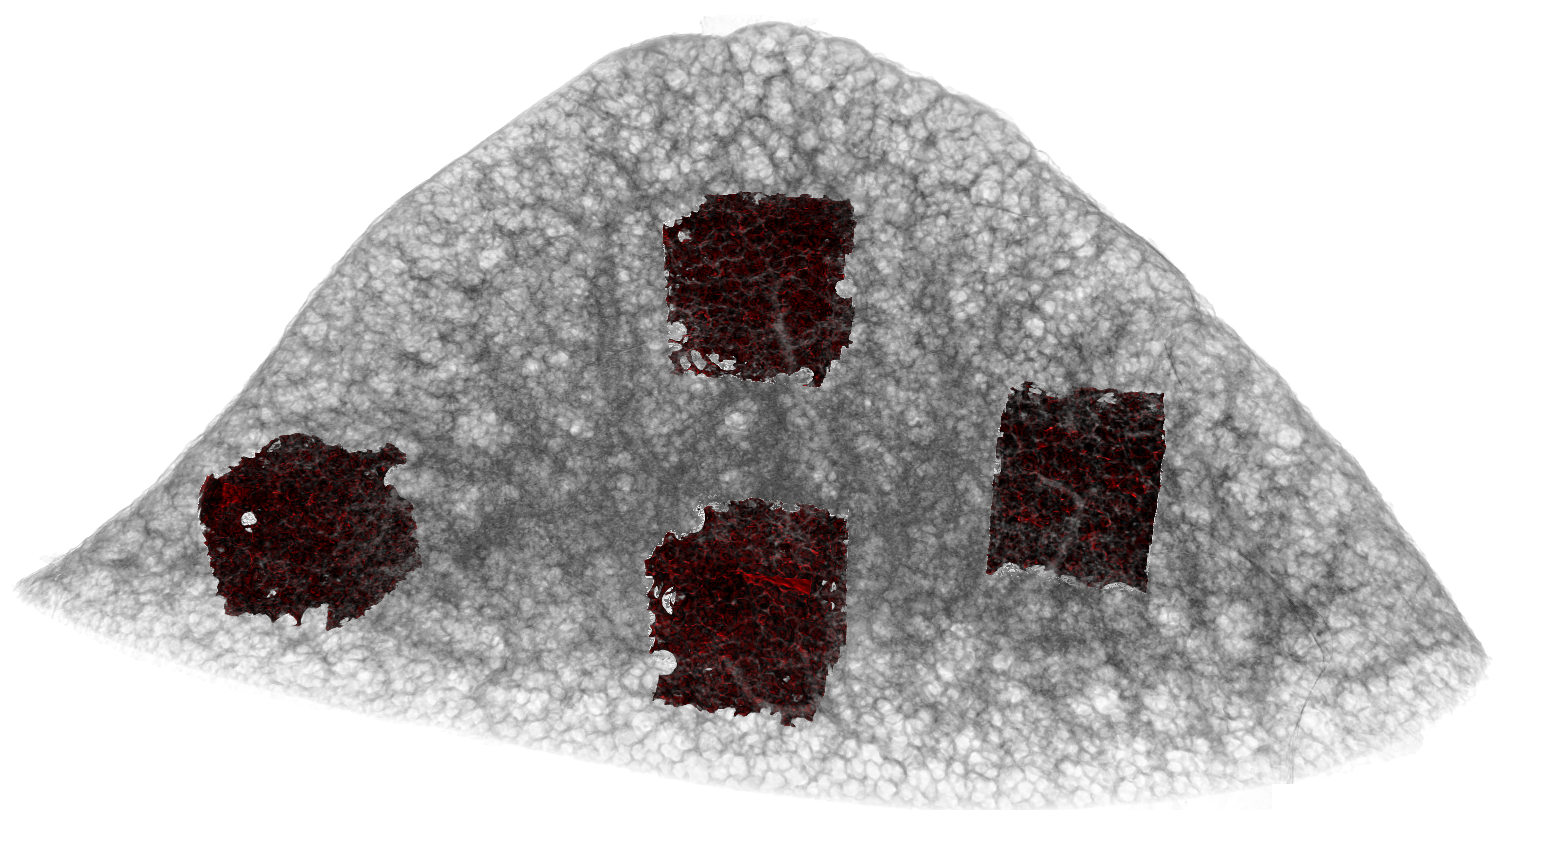
\includegraphics[width=\imagewidth]{../img/dtf-roi/ROIs-3d}};
		% 1357px = 4.0138mm > 100px = 296um > 169px = 500um
		\draw[|-|,thick,red] (83,517) -- (1425,719) node [sloped,midway,below] {\SI{4.0138}{\milli\meter} (2712px)};
		\draw[|-|,thick] (\x-500,\y) -- (\x+169-500,\y) node [midway,above] {\SI{500}{\micro\meter}};
		\draw (368,360) node [fill=white,semitransparent] {ROI 1} node {ROI 1};
		\draw (1038,312) node [fill=white,semitransparent] {ROI 2} node {ROI 2};
		\draw (767,413) node [fill=white,semitransparent] {ROI 3} node {ROI 3};
		\draw (684,139) node [fill=white,semitransparent] {ROI 4} node {ROI 4};
	\end{tikzpicture}%
	\caption{}%
	\label{fig:roi3d}%
\end{figure}

\renewcommand{\imsize}{.618\columnwidth}
\begin{figure}%
	\centering
	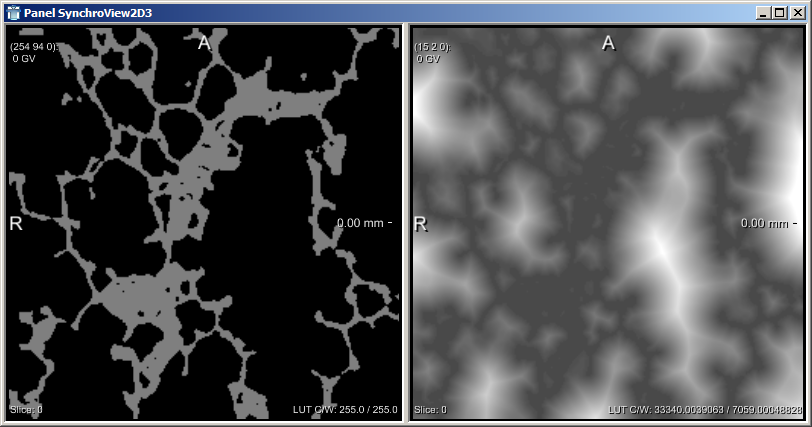
\includegraphics[width=\imsize]{../img/dtf-roi/synchroview}%
	\caption{Left: Thresholded Slice, right: Euclidean distance transformation}%
	\label{fig:synchroview}%
\end{figure}

\renewcommand{\imsize}{\columnwidth}
\begin{figure}%
	\centering
	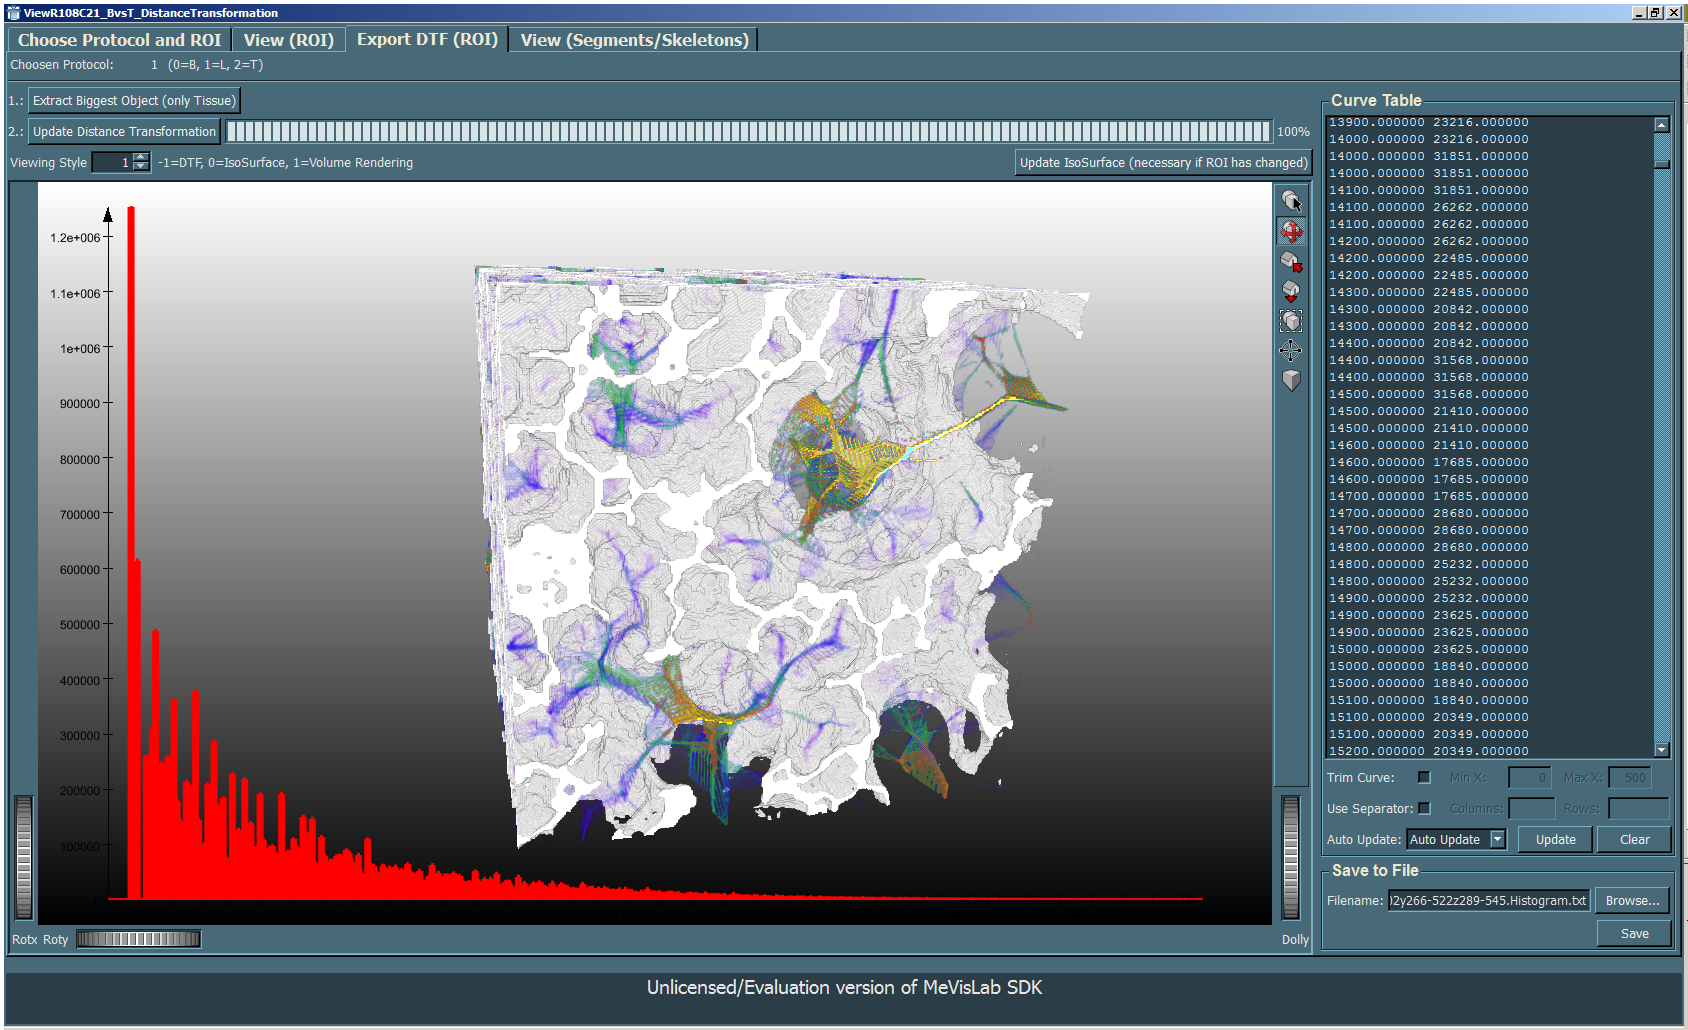
\includegraphics[width=\imsize]{../img/dtf-roi/histogram}%
	\caption{Visualization of ROI, Histogram and local maxima of euclidean distance transformation in the left part of the screenshot, Histogram to be exported in the right part.}%
	\label{fig:GUI}%
\end{figure}

The Histogram of the distance transformation (see figure~\ref{fig:GUI}) has been plotted for each of the 4 ROIs for each of the protocols (B, L and T). Using MATLAB, I've read all those histograms and plotted them (see figure~\ref{fig:MATLABhistograms}). Since it's extremely hard to spot any differences in the distance transformation histograms like this, I overlayed the plots for each region into one plot. Additionally, to better assess the differences in the different histograms, I've chosen a logarithmic scale for the y-axis, since the high values for the larger diameters occlude everything for the smaller diameters.

\renewcommand{\imsize}{\columnwidth}
\begin{figure}%
	\centering
	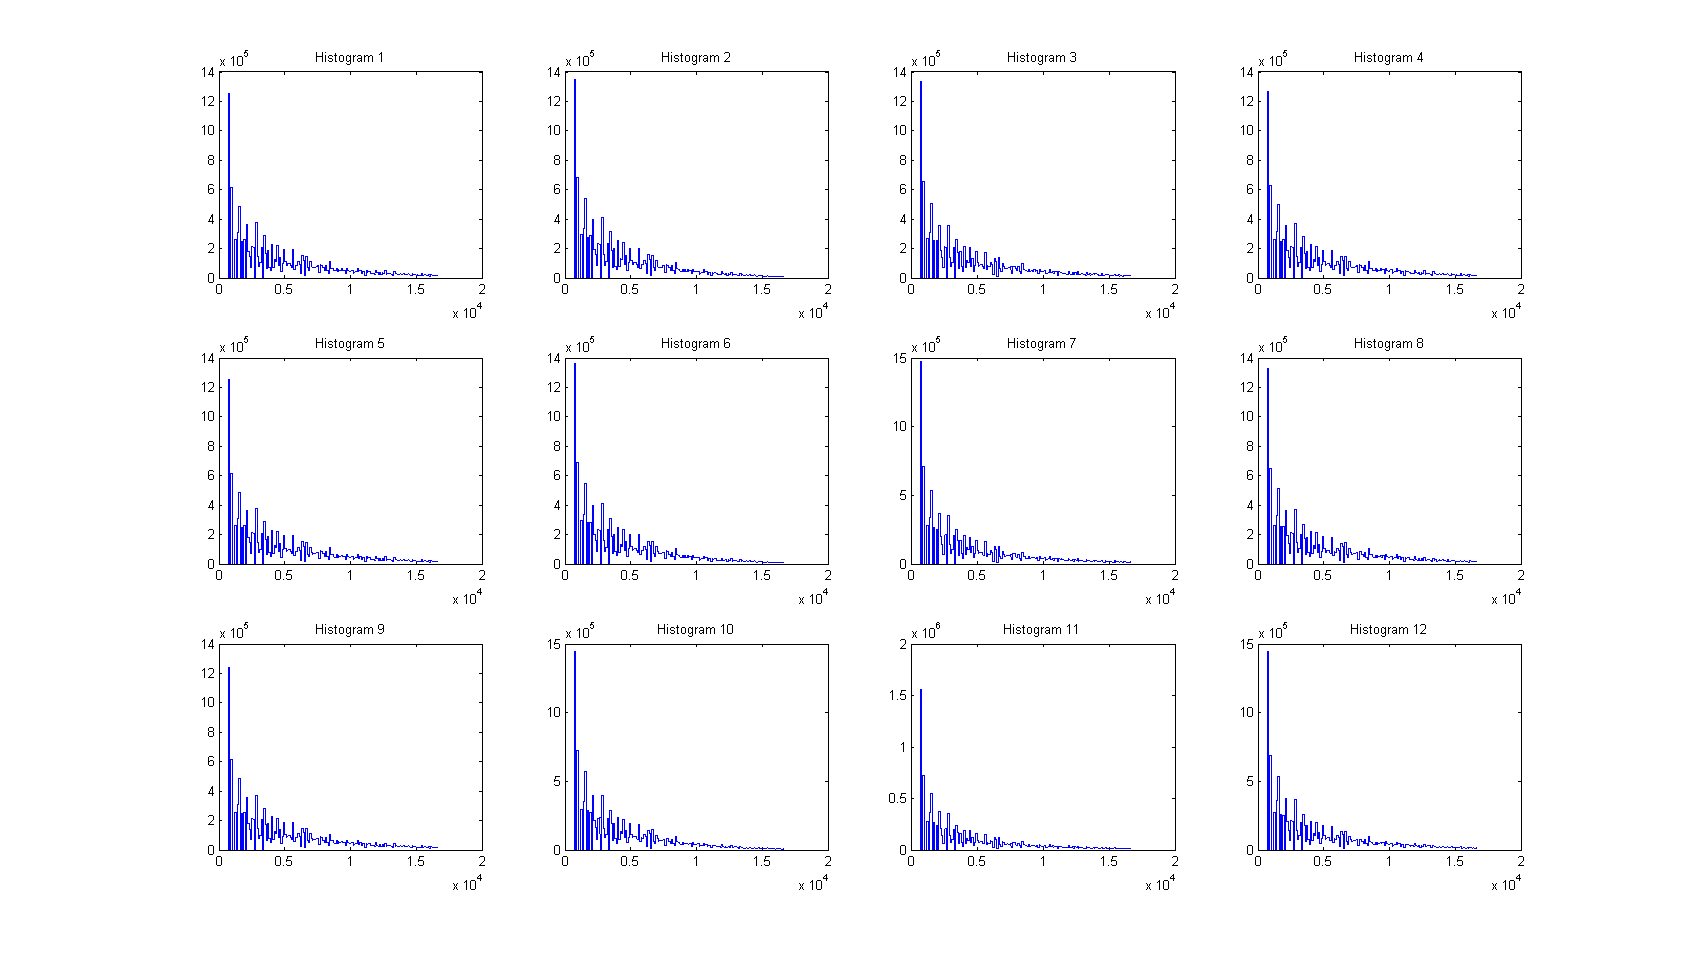
\includegraphics[width=\imsize]{../img/dtf-roi/MATLABhistograms.png}%
	\caption{All Histograms, plotted with MATLAB (Colums: ROIs, Rows: Protocols)}%
	\label{fig:MATLABhistograms}%
\end{figure}


Note that the x-axis has been scaled (in MeVisLab) with $10^6$, so the x-axis-scale is actuall \SI{e-2}{\milli\meter} instead of the stated \SI{e4}{\milli\meter}\ldots For ROI 4, the sum of the histogram is \SI{1.405e7}{pixels}, hence the y-values for the bins are are correct, but we might have some effects of underfilled bins! This is just a quick overview over the histograms, if we use this, there will be some more finetuning.

Figure~\ref{fig:plots} shows a plot for each of the ROIs; the \textcolor{blue}{blue} plot shows the logarithmic histogram of the distance transformation of Protocol B, the \textcolor{green}{green} and \textcolor{red}{red} plot the same for protocols L and T, respectively. A discernible difference is only visible for the larger diameters ($>$\SI{3e-2}{\milli\meter} and even there only for ROIs 3 and 4.

\begin{figure}%
	\subfloat[ROI 1]{% \documentclass{article}
% \usepackage{tikz,pgfplots}
% \usepackage[pdftex,active,tightpage]{preview}
% \begin{document}
% \begin{preview}
%%%%%%%%%%%%
\begin{tikzpicture}

% Axis at [0.13 0.11 0.78 0.81]
\begin{semilogyaxis}[
%axis on top,
%scale only axis,
%width=.5\linewidth,
xmin=0, xmax=42500,
ymin=1, ymax=1e+006,
%title={ROI 1},
legend entries={%
%	B.x1146-1402y266-522z289-545.txt,
%	L.x1146-1402y266-522z289-545.txt,
%	T.x1146-1402y266-522z289-545.txt%
	B (ROI 1),
	L (ROI 1),
	T (ROI 1)%
	}
]

%\pgfplotsset{every axis legend/.append style={at={(0,-.18)},anchor=north west}}

\addplot [
color=blue,
solid
]coordinates{
 (3400,0) (3400,289501) (3400,289501) (3500,289501) (3500,168870) (3500,168870) (3600,168870) (3600,65511) (3600,65511) (3700,65511) (3700,185453) (3700,185453) (3800,185453) (3800,74694) (3800,74694) (3900,74694) (3900,52846) (3900,52846) (4000,52846) (4000,230325) (4000,230325) (4100,230325) (4100,70838) (4100,70838) (4200,70838) (4200,127584) (4200,127584) (4300,127584) (4300,112007) (4300,112007) (4400,112007) (4400,220564) (4400,220564) (4500,220564) (4500,83095) (4500,83095) (4600,83095) (4600,140906) (4600,140906) (4700,140906) (4700,46921) (4700,46921) (4800,46921) (4800,98956) (4800,98956) (4900,98956) (4900,191119) (4900,191119) (5000,191119) (5000,109497) (5000,109497) (5100,109497) (5100,83683) (5100,83683) (5200,83683) (5200,95212) (5200,95212) (5300,95212) (5300,98242) (5300,98242) (5400,98242) (5400,85358) (5400,85358) (5500,85358) (5500,69667) (5500,69667) (5600,69667) (5600,193089) (5600,193089) (5700,193089) (5700,60959) (5700,60959) (5800,60959) (5800,87206) (5800,87206) (5900,87206) (5900,88163) (5900,88163) (6000,88163) (6000,111357) (6000,111357) (6100,111357) (6100,94851) (6100,94851) (6200,94851) (6200,28137) (6200,28137) (6300,28137) (6300,151541) (6300,151541) (6400,151541) (6400,121345) (6400,121345) (6500,121345) (6500,14476) (6500,14476) (6600,14476) (6600,148633) (6600,148633) (6700,148633) (6700,68210) (6700,68210) (6800,68210) (6800,51398) (6800,51398) (6900,51398) (6900,114875) (6900,114875) (7000,114875) (7000,79729) (7000,79729) (7100,79729) (7100,68479) (7100,68479) (7200,68479) (7200,72250) (7200,72250) (7300,72250) (7300,72049) (7300,72049) (7400,72049) (7400,79753) (7400,79753) (7500,79753) (7500,81664) (7500,81664) (7600,81664) (7600,34829) (7600,34829) (7700,34829) (7700,90607) (7700,90607) (7800,90607) (7800,86063) (7800,86063) (7900,86063) (7900,69170) (7900,69170) (8000,69170) (8000,53271) (8000,53271) (8100,53271) (8100,83343) (8100,83343) (8200,83343) (8200,49082) (8200,49082) (8300,49082) (8300,32539) (8300,32539) (8400,32539) (8400,111026) (8400,111026) (8500,111026) (8500,63768) (8500,63768) (8600,63768) (8600,62827) (8600,62827) (8700,62827) (8700,51868) (8700,51868) (8800,51868) (8800,48185) (8800,48185) (8900,48185) (8900,62312) (8900,62312) (9000,62312) (9000,45697) (9000,45697) (9100,45697) (9100,59199) (9100,59199) (9200,59199) (9200,50125) (9200,50125) (9300,50125) (9300,61532) (9300,61532) (9400,61532) (9400,48789) (9400,48789) (9500,48789) (9500,54360) (9500,54360) (9600,54360) (9600,32444) (9600,32444) (9700,32444) (9700,65857) (9700,65857) (9800,65857) (9800,51861) (9800,51861) (9900,51861) (9900,45863) (9900,45863) (10000,45863) (10000,47039) (10000,47039) (10100,47039) (10100,53244) (10100,53244) (10200,53244) (10200,30468) (10200,30468) (10300,30468) (10300,36249) (10300,36249) (10400,36249) (10400,43946) (10400,43946) (10500,43946) (10500,63584) (10500,63584) (10600,63584) (10600,40905) (10600,40905) (10700,40905) (10700,49551) (10700,49551) (10800,49551) (10800,31017) (10800,31017) (10900,31017) (10900,44626) (10900,44626) (11000,44626) (11000,45134) (11000,45134) (11100,45134) (11100,19390) (11100,19390) (11200,19390) (11200,48419) (11200,48419) (11300,48419) (11300,40598) (11300,40598) (11400,40598) (11400,43419) (11400,43419) (11500,43419) (11500,33352) (11500,33352) (11600,33352) (11600,31319) (11600,31319) (11700,31319) (11700,32941) (11700,32941) (11800,32941) (11800,27127) (11800,27127) (11900,27127) (11900,52285) (11900,52285) (12000,52285) (12000,34413) (12000,34413) (12100,34413) (12100,27138) (12100,27138) (12200,27138) (12200,38339) (12200,38339) (12300,38339) (12300,24127) (12300,24127) (12400,24127) (12400,38567) (12400,38567) (12500,38567) (12500,27187) (12500,27187) (12600,27187) (12600,48367) (12600,48367) (12700,48367) (12700,24372) (12700,24372) (12800,24372) (12800,28211) (12800,28211) (12900,28211) (12900,32657) (12900,32657) (13000,32657) (13000,33653) (13000,33653) (13100,33653) (13100,23533) (13100,23533) (13200,23533) (13200,19206) (13200,19206) (13300,19206) (13300,42551) (13300,42551) (13400,42551) (13400,27399) (13400,27399) (13500,27399) (13500,31332) (13500,31332) (13600,31332) (13600,21042) (13600,21042) (13700,21042) (13700,23662) (13700,23662) (13800,23662) (13800,30551) (13800,30551) (13900,30551) (13900,23126) (13900,23126) (14000,23126) (14000,32415) (14000,32415) (14100,32415) (14100,26522) (14100,26522) (14200,26522) (14200,22807) (14200,22807) (14300,22807) (14300,20796) (14300,20796) (14400,20796) (14400,31838) (14400,31838) (14500,31838) (14500,21486) (14500,21486) (14600,21486) (14600,17839) (14600,17839) (14700,17839) (14700,29346) (14700,29346) (14800,29346) (14800,25394) (14800,25394) (14900,25394) (14900,23931) (14900,23931) (15000,23931) (15000,19010) (15000,19010) (15100,19010) (15100,20692) (15100,20692) (15200,20692) (15200,19154) (15200,19154) (15300,19154) (15300,18638) (15300,18638) (15400,18638) (15400,29391) (15400,29391) (15500,29391) (15500,15838) (15500,15838) (15600,15838) (15600,21447) (15600,21447) (15700,21447) (15700,22688) (15700,22688) (15800,22688) (15800,15210) (15800,15210) (15900,15210) (15900,21187) (15900,21187) (16000,21187) (16000,13291) (16000,13291) (16100,13291) (16100,22614) (16100,22614) (16200,22614) (16200,19969) (16200,19969) (16300,19969) (16300,16789) (16300,16789) (16400,16789) (16400,17367) (16400,17367) (16500,17367) (16500,15681) (16500,15681) (16600,15681) (16600,19884) (16600,19884) (16700,19884) (16700,9854) (16700,9854) (16800,9854) (16800,20652) (16800,20652) (16900,20652) (16900,16546) (16900,16546) (17000,16546) (17000,16711) (17000,16711) (17100,16711) (17100,13728) (17100,13728) (17200,13728) (17200,12229) (17200,12229) (17300,12229) (17300,15340) (17300,15340) (17400,15340) (17400,10601) (17400,10601) (17500,10601) (17500,20681) (17500,20681) (17600,20681) (17600,12315) (17600,12315) (17700,12315) (17700,14426) (17700,14426) (17800,14426) (17800,12931) (17800,12931) (17900,12931) (17900,14507) (17900,14507) (18000,14507) (18000,11234) (18000,11234) (18100,11234) (18100,11937) (18100,11937) (18200,11937) (18200,13626) (18200,13626) (18300,13626) (18300,13537) (18300,13537) (18400,13537) (18400,11925) (18400,11925) (18500,11925) (18500,12930) (18500,12930) (18600,12930) (18600,9601) (18600,9601) (18700,9601) (18700,9149) (18700,9149) (18800,9149) (18800,10962) (18800,10962) (18900,10962) (18900,12041) (18900,12041) (19000,12041) (19000,10697) (19000,10697) (19100,10697) (19100,11133) (19100,11133) (19200,11133) (19200,9424) (19200,9424) (19300,9424) (19300,9013) (19300,9013) (19400,9013) (19400,12315) (19400,12315) (19500,12315) (19500,7887) (19500,7887) (19600,7887) (19600,9301) (19600,9301) (19700,9301) (19700,9182) (19700,9182) (19800,9182) (19800,9502) (19800,9502) (19900,9502) (19900,7621) (19900,7621) (20000,7621) (20000,9584) (20000,9584) (20100,9584) (20100,6208) (20100,6208) (20200,6208) (20200,7255) (20200,7255) (20300,7255) (20300,11315) (20300,11315) (20400,11315) (20400,8066) (20400,8066) (20500,8066) (20500,7519) (20500,7519) (20600,7519) (20600,6584) (20600,6584) (20700,6584) (20700,6964) (20700,6964) (20800,6964) (20800,6797) (20800,6797) (20900,6797) (20900,5566) (20900,5566) (21000,5566) (21000,7473) (21000,7473) (21100,7473) (21100,7186) (21100,7186) (21200,7186) (21200,5091) (21200,5091) (21300,5091) (21300,7039) (21300,7039) (21400,7039) (21400,5524) (21400,5524) (21500,5524) (21500,5297) (21500,5297) (21600,5297) (21600,4091) (21600,4091) (21700,4091) (21700,7392) (21700,7392) (21800,7392) (21800,5227) (21800,5227) (21900,5227) (21900,5764) (21900,5764) (22000,5764) (22000,4223) (22000,4223) (22100,4223) (22100,4689) (22100,4689) (22200,4689) (22200,4919) (22200,4919) (22300,4919) (22300,4045) (22300,4045) (22400,4045) (22400,5036) (22400,5036) (22500,5036) (22500,4647) (22500,4647) (22600,4647) (22600,4661) (22600,4661) (22700,4661) (22700,3201) (22700,3201) (22800,3201) (22800,5155) (22800,5155) (22900,5155) (22900,3256) (22900,3256) (23000,3256) (23000,3062) (23000,3062) (23100,3062) (23100,5112) (23100,5112) (23200,5112) (23200,3688) (23200,3688) (23300,3688) (23300,3215) (23300,3215) (23400,3215) (23400,3841) (23400,3841) (23500,3841) (23500,3096) (23500,3096) (23600,3096) (23600,3620) (23600,3620) (23700,3620) (23700,2830) (23700,2830) (23800,2830) (23800,3711) (23800,3711) (23900,3711) (23900,3323) (23900,3323) (24000,3323) (24000,2678) (24000,2678) (24100,2678) (24100,3506) (24100,3506) (24200,3506) (24200,2545) (24200,2545) (24300,2545) (24300,2722) (24300,2722) (24400,2722) (24400,2407) (24400,2407) (24500,2407) (24500,3437) (24500,3437) (24600,3437) (24600,2471) (24600,2471) (24700,2471) (24700,2523) (24700,2523) (24800,2523) (24800,2558) (24800,2558) (24900,2558) (24900,2415) (24900,2415) (25000,2415) (25000,1949) (25000,1949) (25100,1949) (25100,2253) (25100,2253) (25200,2253) (25200,2855) (25200,2855) (25300,2855) (25300,2187) (25300,2187) (25400,2187) (25400,2267) (25400,2267) (25500,2267) (25500,1759) (25500,1759) (25600,1759) (25600,1684) (25600,1684) (25700,1684) (25700,2203) (25700,2203) (25800,2203) (25800,1671) (25800,1671) (25900,1671) (25900,2267) (25900,2267) (26000,2267) (26000,2018) (26000,2018) (26100,2018) (26100,1378) (26100,1378) (26200,1378) (26200,1776) (26200,1776) (26300,1776) (26300,1973) (26300,1973) (26400,1973) (26400,1539) (26400,1539) (26500,1539) (26500,1075) (26500,1075) (26600,1075) (26600,2143) (26600,2143) (26700,2143) (26700,1159) (26700,1159) (26800,1159) (26800,1639) (26800,1639) (26900,1639) (26900,1331) (26900,1331) (27000,1331) (27000,1411) (27000,1411) (27100,1411) (27100,1181) (27100,1181) (27200,1181) (27200,1310) (27200,1310) (27300,1310) (27300,1538) (27300,1538) (27400,1538) (27400,1074) (27400,1074) (27500,1074) (27500,1274) (27500,1274) (27600,1274) (27600,989) (27600,989) (27700,989) (27700,1195) (27700,1195) (27800,1195) (27800,906) (27800,906) (27900,906) (27900,1026) (27900,1026) (28000,1026) (28000,1201) (28000,1201) (28100,1201) (28100,959) (28100,959) (28200,959) (28200,987) (28200,987) (28300,987) (28300,924) (28300,924) (28400,924) (28400,667) (28400,667) (28500,667) (28500,941) (28500,941) (28600,941) (28600,544) (28600,544) (28700,544) (28700,1026) (28700,1026) (28800,1026) (28800,842) (28800,842) (28900,842) (28900,726) (28900,726) (29000,726) (29000,573) (29000,573) (29100,573) (29100,717) (29100,717) (29200,717) (29200,638) (29200,638) (29300,638) (29300,597) (29300,597) (29400,597) (29400,693) (29400,693) (29500,693) (29500,657) (29500,657) (29600,657) (29600,480) (29600,480) (29700,480) (29700,673) (29700,673) (29800,673) (29800,466) (29800,466) (29900,466) (29900,580) (29900,580) (30000,580) (30000,414) (30000,414) (30100,414) (30100,657) (30100,657) (30200,657) (30200,454) (30200,454) (30300,454) (30300,591) (30300,591) (30400,591) (30400,422) (30400,422) (30500,422) (30500,428) (30500,428) (30600,428) (30600,353) (30600,353) (30700,353) (30700,452) (30700,452) (30800,452) (30800,483) (30800,483) (30900,483) (30900,413) (30900,413) (31000,413) (31000,411) (31000,411) (31100,411) (31100,320) (31100,320) (31200,320) (31200,397) (31200,397) (31300,397) (31300,359) (31300,359) (31400,359) (31400,305) (31400,305) (31500,305) (31500,328) (31500,328) (31600,328) (31600,358) (31600,358) (31700,358) (31700,319) (31700,319) (31800,319) (31800,291) (31800,291) (31900,291) (31900,284) (31900,284) (32000,284) (32000,234) (32000,234) (32100,234) (32100,220) (32100,220) (32200,220) (32200,344) (32200,344) (32300,344) (32300,265) (32300,265) (32400,265) (32400,191) (32400,191) (32500,191) (32500,161) (32500,161) (32600,161) (32600,231) (32600,231) (32700,231) (32700,155) (32700,155) (32800,155) (32800,171) (32800,171) (32900,171) (32900,234) (32900,234) (33000,234) (33000,129) (33000,129) (33100,129) (33100,116) (33100,116) (33200,116) (33200,157) (33200,157) (33300,157) (33300,116) (33300,116) (33400,116) (33400,88) (33400,88) (33500,88) (33500,85) (33500,85) (33600,85) (33600,96) (33600,96) (33700,96) (33700,80) (33700,80) (33800,80) (33800,82) (33800,82) (33900,82) (33900,57) (33900,57) (34000,57) (34000,35) (34000,35) (34100,35) (34100,46) (34100,46) (34200,46) (34200,36) (34200,36) (34300,36) (34300,29) (34300,29) (34400,29) (34400,21) (34400,21) (34500,21) (34500,16) (34500,16) (34600,16) (34600,16) (34600,16) (34700,16) (34700,14) (34700,14) (34800,14) (34800,9) (34800,9) (34900,9) (34900,9) (34900,9) (35000,9) (35000,10) (35000,10) (35100,10) (35100,4) (35100,4) (35200,4) (35200,4) (35200,4) (35300,4) (35300,2) (35300,2) (35400,2) (35400,1)
};

\addplot [
color=green,
solid
]coordinates{
 (3400,0) (3400,285587) (3400,285587) (3500,285587) (3500,169714) (3500,169714) (3600,169714) (3600,65682) (3600,65682) (3700,65682) (3700,183620) (3700,183620) (3800,183620) (3800,75379) (3800,75379) (3900,75379) (3900,51642) (3900,51642) (4000,51642) (4000,227882) (4000,227882) (4100,227882) (4100,71053) (4100,71053) (4200,71053) (4200,127295) (4200,127295) (4300,127295) (4300,111638) (4300,111638) (4400,111638) (4400,218480) (4400,218480) (4500,218480) (4500,82720) (4500,82720) (4600,82720) (4600,139178) (4600,139178) (4700,139178) (4700,47263) (4700,47263) (4800,47263) (4800,97436) (4800,97436) (4900,97436) (4900,190870) (4900,190870) (5000,190870) (5000,108250) (5000,108250) (5100,108250) (5100,83492) (5100,83492) (5200,83492) (5200,94695) (5200,94695) (5300,94695) (5300,96844) (5300,96844) (5400,96844) (5400,84074) (5400,84074) (5500,84074) (5500,69652) (5500,69652) (5600,69652) (5600,191832) (5600,191832) (5700,191832) (5700,60244) (5700,60244) (5800,60244) (5800,86981) (5800,86981) (5900,86981) (5900,86728) (5900,86728) (6000,86728) (6000,110216) (6000,110216) (6100,110216) (6100,94312) (6100,94312) (6200,94312) (6200,27164) (6200,27164) (6300,27164) (6300,150953) (6300,150953) (6400,150953) (6400,120343) (6400,120343) (6500,120343) (6500,14202) (6500,14202) (6600,14202) (6600,147009) (6600,147009) (6700,147009) (6700,67351) (6700,67351) (6800,67351) (6800,49810) (6800,49810) (6900,49810) (6900,114108) (6900,114108) (7000,114108) (7000,79775) (7000,79775) (7100,79775) (7100,67677) (7100,67677) (7200,67677) (7200,71054) (7200,71054) (7300,71054) (7300,71112) (7300,71112) (7400,71112) (7400,78892) (7400,78892) (7500,78892) (7500,80222) (7500,80222) (7600,80222) (7600,34643) (7600,34643) (7700,34643) (7700,90088) (7700,90088) (7800,90088) (7800,84851) (7800,84851) (7900,84851) (7900,68051) (7900,68051) (8000,68051) (8000,52909) (8000,52909) (8100,52909) (8100,81863) (8100,81863) (8200,81863) (8200,48703) (8200,48703) (8300,48703) (8300,32105) (8300,32105) (8400,32105) (8400,109750) (8400,109750) (8500,109750) (8500,63514) (8500,63514) (8600,63514) (8600,62172) (8600,62172) (8700,62172) (8700,50881) (8700,50881) (8800,50881) (8800,47091) (8800,47091) (8900,47091) (8900,62039) (8900,62039) (9000,62039) (9000,44968) (9000,44968) (9100,44968) (9100,58587) (9100,58587) (9200,58587) (9200,49966) (9200,49966) (9300,49966) (9300,60443) (9300,60443) (9400,60443) (9400,48528) (9400,48528) (9500,48528) (9500,53901) (9500,53901) (9600,53901) (9600,32302) (9600,32302) (9700,32302) (9700,64503) (9700,64503) (9800,64503) (9800,51449) (9800,51449) (9900,51449) (9900,45907) (9900,45907) (10000,45907) (10000,46182) (10000,46182) (10100,46182) (10100,52795) (10100,52795) (10200,52795) (10200,30334) (10200,30334) (10300,30334) (10300,35498) (10300,35498) (10400,35498) (10400,43463) (10400,43463) (10500,43463) (10500,63129) (10500,63129) (10600,63129) (10600,40290) (10600,40290) (10700,40290) (10700,49459) (10700,49459) (10800,49459) (10800,30485) (10800,30485) (10900,30485) (10900,44159) (10900,44159) (11000,44159) (11000,44784) (11000,44784) (11100,44784) (11100,19043) (11100,19043) (11200,19043) (11200,48026) (11200,48026) (11300,48026) (11300,40100) (11300,40100) (11400,40100) (11400,43361) (11400,43361) (11500,43361) (11500,33092) (11500,33092) (11600,33092) (11600,30961) (11600,30961) (11700,30961) (11700,32607) (11700,32607) (11800,32607) (11800,26918) (11800,26918) (11900,26918) (11900,51725) (11900,51725) (12000,51725) (12000,34420) (12000,34420) (12100,34420) (12100,27015) (12100,27015) (12200,27015) (12200,37899) (12200,37899) (12300,37899) (12300,23839) (12300,23839) (12400,23839) (12400,38670) (12400,38670) (12500,38670) (12500,26977) (12500,26977) (12600,26977) (12600,47886) (12600,47886) (12700,47886) (12700,24290) (12700,24290) (12800,24290) (12800,27865) (12800,27865) (12900,27865) (12900,32681) (12900,32681) (13000,32681) (13000,33349) (13000,33349) (13100,33349) (13100,23303) (13100,23303) (13200,23303) (13200,19055) (13200,19055) (13300,19055) (13300,42280) (13300,42280) (13400,42280) (13400,27188) (13400,27188) (13500,27188) (13500,31068) (13500,31068) (13600,31068) (13600,20995) (13600,20995) (13700,20995) (13700,23250) (13700,23250) (13800,23250) (13800,30452) (13800,30452) (13900,30452) (13900,23216) (13900,23216) (14000,23216) (14000,31851) (14000,31851) (14100,31851) (14100,26262) (14100,26262) (14200,26262) (14200,22485) (14200,22485) (14300,22485) (14300,20842) (14300,20842) (14400,20842) (14400,31568) (14400,31568) (14500,31568) (14500,21410) (14500,21410) (14600,21410) (14600,17685) (14600,17685) (14700,17685) (14700,28680) (14700,28680) (14800,28680) (14800,25232) (14800,25232) (14900,25232) (14900,23625) (14900,23625) (15000,23625) (15000,18840) (15000,18840) (15100,18840) (15100,20349) (15100,20349) (15200,20349) (15200,18791) (15200,18791) (15300,18791) (15300,18512) (15300,18512) (15400,18512) (15400,28981) (15400,28981) (15500,28981) (15500,15601) (15500,15601) (15600,15601) (15600,20967) (15600,20967) (15700,20967) (15700,22281) (15700,22281) (15800,22281) (15800,15077) (15800,15077) (15900,15077) (15900,20798) (15900,20798) (16000,20798) (16000,13211) (16000,13211) (16100,13211) (16100,22204) (16100,22204) (16200,22204) (16200,19528) (16200,19528) (16300,19528) (16300,16521) (16300,16521) (16400,16521) (16400,17226) (16400,17226) (16500,17226) (16500,15381) (16500,15381) (16600,15381) (16600,19527) (16600,19527) (16700,19527) (16700,9783) (16700,9783) (16800,9783) (16800,20502) (16800,20502) (16900,20502) (16900,16286) (16900,16286) (17000,16286) (17000,16331) (17000,16331) (17100,16331) (17100,13462) (17100,13462) (17200,13462) (17200,11926) (17200,11926) (17300,11926) (17300,15227) (17300,15227) (17400,15227) (17400,10583) (17400,10583) (17500,10583) (17500,20302) (17500,20302) (17600,20302) (17600,11984) (17600,11984) (17700,11984) (17700,13994) (17700,13994) (17800,13994) (17800,12825) (17800,12825) (17900,12825) (17900,14359) (17900,14359) (18000,14359) (18000,11078) (18000,11078) (18100,11078) (18100,11732) (18100,11732) (18200,11732) (18200,13287) (18200,13287) (18300,13287) (18300,13401) (18300,13401) (18400,13401) (18400,11693) (18400,11693) (18500,11693) (18500,12642) (18500,12642) (18600,12642) (18600,9455) (18600,9455) (18700,9455) (18700,8944) (18700,8944) (18800,8944) (18800,10839) (18800,10839) (18900,10839) (18900,11862) (18900,11862) (19000,11862) (19000,10426) (19000,10426) (19100,10426) (19100,10817) (19100,10817) (19200,10817) (19200,9237) (19200,9237) (19300,9237) (19300,8842) (19300,8842) (19400,8842) (19400,12068) (19400,12068) (19500,12068) (19500,7734) (19500,7734) (19600,7734) (19600,9009) (19600,9009) (19700,9009) (19700,8824) (19700,8824) (19800,8824) (19800,9234) (19800,9234) (19900,9234) (19900,7496) (19900,7496) (20000,7496) (20000,9337) (20000,9337) (20100,9337) (20100,6054) (20100,6054) (20200,6054) (20200,7045) (20200,7045) (20300,7045) (20300,11020) (20300,11020) (20400,11020) (20400,7832) (20400,7832) (20500,7832) (20500,7268) (20500,7268) (20600,7268) (20600,6314) (20600,6314) (20700,6314) (20700,6675) (20700,6675) (20800,6675) (20800,6701) (20800,6701) (20900,6701) (20900,5453) (20900,5453) (21000,5453) (21000,7241) (21000,7241) (21100,7241) (21100,6856) (21100,6856) (21200,6856) (21200,4903) (21200,4903) (21300,4903) (21300,6899) (21300,6899) (21400,6899) (21400,5384) (21400,5384) (21500,5384) (21500,5093) (21500,5093) (21600,5093) (21600,3919) (21600,3919) (21700,3919) (21700,7087) (21700,7087) (21800,7087) (21800,5140) (21800,5140) (21900,5140) (21900,5584) (21900,5584) (22000,5584) (22000,4113) (22000,4113) (22100,4113) (22100,4524) (22100,4524) (22200,4524) (22200,4706) (22200,4706) (22300,4706) (22300,3951) (22300,3951) (22400,3951) (22400,4904) (22400,4904) (22500,4904) (22500,4486) (22500,4486) (22600,4486) (22600,4478) (22600,4478) (22700,4478) (22700,3105) (22700,3105) (22800,3105) (22800,4990) (22800,4990) (22900,4990) (22900,3121) (22900,3121) (23000,3121) (23000,2940) (23000,2940) (23100,2940) (23100,4888) (23100,4888) (23200,4888) (23200,3596) (23200,3596) (23300,3596) (23300,3131) (23300,3131) (23400,3131) (23400,3638) (23400,3638) (23500,3638) (23500,2989) (23500,2989) (23600,2989) (23600,3418) (23600,3418) (23700,3418) (23700,2727) (23700,2727) (23800,2727) (23800,3595) (23800,3595) (23900,3595) (23900,3212) (23900,3212) (24000,3212) (24000,2540) (24000,2540) (24100,2540) (24100,3348) (24100,3348) (24200,3348) (24200,2493) (24200,2493) (24300,2493) (24300,2621) (24300,2621) (24400,2621) (24400,2243) (24400,2243) (24500,2243) (24500,3329) (24500,3329) (24600,3329) (24600,2395) (24600,2395) (24700,2395) (24700,2465) (24700,2465) (24800,2465) (24800,2478) (24800,2478) (24900,2478) (24900,2275) (24900,2275) (25000,2275) (25000,1818) (25000,1818) (25100,1818) (25100,2114) (25100,2114) (25200,2114) (25200,2792) (25200,2792) (25300,2792) (25300,2130) (25300,2130) (25400,2130) (25400,2147) (25400,2147) (25500,2147) (25500,1690) (25500,1690) (25600,1690) (25600,1572) (25600,1572) (25700,1572) (25700,2162) (25700,2162) (25800,2162) (25800,1563) (25800,1563) (25900,1563) (25900,2129) (25900,2129) (26000,2129) (26000,1893) (26000,1893) (26100,1893) (26100,1346) (26100,1346) (26200,1346) (26200,1765) (26200,1765) (26300,1765) (26300,1829) (26300,1829) (26400,1829) (26400,1439) (26400,1439) (26500,1439) (26500,1003) (26500,1003) (26600,1003) (26600,2001) (26600,2001) (26700,2001) (26700,1149) (26700,1149) (26800,1149) (26800,1565) (26800,1565) (26900,1565) (26900,1226) (26900,1226) (27000,1226) (27000,1335) (27000,1335) (27100,1335) (27100,1065) (27100,1065) (27200,1065) (27200,1313) (27200,1313) (27300,1313) (27300,1425) (27300,1425) (27400,1425) (27400,1005) (27400,1005) (27500,1005) (27500,1165) (27500,1165) (27600,1165) (27600,931) (27600,931) (27700,931) (27700,1177) (27700,1177) (27800,1177) (27800,841) (27800,841) (27900,841) (27900,968) (27900,968) (28000,968) (28000,1062) (28000,1062) (28100,1062) (28100,884) (28100,884) (28200,884) (28200,990) (28200,990) (28300,990) (28300,827) (28300,827) (28400,827) (28400,621) (28400,621) (28500,621) (28500,851) (28500,851) (28600,851) (28600,512) (28600,512) (28700,512) (28700,965) (28700,965) (28800,965) (28800,779) (28800,779) (28900,779) (28900,624) (28900,624) (29000,624) (29000,522) (29000,522) (29100,522) (29100,649) (29100,649) (29200,649) (29200,679) (29200,679) (29300,679) (29300,548) (29300,548) (29400,548) (29400,629) (29400,629) (29500,629) (29500,569) (29500,569) (29600,569) (29600,484) (29600,484) (29700,484) (29700,638) (29700,638) (29800,638) (29800,410) (29800,410) (29900,410) (29900,512) (29900,512) (30000,512) (30000,371) (30000,371) (30100,371) (30100,640) (30100,640) (30200,640) (30200,418) (30200,418) (30300,418) (30300,511) (30300,511) (30400,511) (30400,364) (30400,364) (30500,364) (30500,393) (30500,393) (30600,393) (30600,373) (30600,373) (30700,373) (30700,426) (30700,426) (30800,426) (30800,414) (30800,414) (30900,414) (30900,353) (30900,353) (31000,353) (31000,355) (31000,355) (31100,355) (31100,367) (31100,367) (31200,367) (31200,348) (31200,348) (31300,348) (31300,322) (31300,322) (31400,322) (31400,267) (31400,267) (31500,267) (31500,289) (31500,289) (31600,289) (31600,362) (31600,362) (31700,362) (31700,311) (31700,311) (31800,311) (31800,240) (31800,240) (31900,240) (31900,233) (31900,233) (32000,233) (32000,221) (32000,221) (32100,221) (32100,242) (32100,242) (32200,242) (32200,326) (32200,326) (32300,326) (32300,214) (32300,214) (32400,214) (32400,165) (32400,165) (32500,165) (32500,144) (32500,144) (32600,144) (32600,254) (32600,254) (32700,254) (32700,133) (32700,133) (32800,133) (32800,143) (32800,143) (32900,143) (32900,206) (32900,206) (33000,206) (33000,112) (33000,112) (33100,112) (33100,130) (33100,130) (33200,130) (33200,133) (33200,133) (33300,133) (33300,98) (33300,98) (33400,98) (33400,74) (33400,74) (33500,74) (33500,88) (33500,88) (33600,88) (33600,104) (33600,104) (33700,104) (33700,79) (33700,79) (33800,79) (33800,79) (33800,79) (33900,79) (33900,49) (33900,49) (34000,49) (34000,35) (34000,35) (34100,35) (34100,61) (34100,61) (34200,61) (34200,52) (34200,52) (34300,52) (34300,26) (34300,26) (34400,26) (34400,26) (34400,26) (34500,26) (34500,14) (34500,14) (34600,14) (34600,11) (34600,11) (34700,11) (34700,14) (34700,14) (34800,14) (34800,11) (34800,11) (34900,11) (34900,9) (34900,9) (35000,9) (35000,4) (35000,4) (35100,4) (35100,2) (35100,2) (35200,2) (35200,4) (35200,4) (35300,4) (35300,1)
};

\addplot [
color=red,
solid
]coordinates{
 (3400,0) (3400,280054) (3400,280054) (3500,280054) (3500,171184) (3500,171184) (3600,171184) (3600,65309) (3600,65309) (3700,65309) (3700,182699) (3700,182699) (3800,182699) (3800,75927) (3800,75927) (3900,75927) (3900,50874) (3900,50874) (4000,50874) (4000,225669) (4000,225669) (4100,225669) (4100,71324) (4100,71324) (4200,71324) (4200,125610) (4200,125610) (4300,125610) (4300,110775) (4300,110775) (4400,110775) (4400,217173) (4400,217173) (4500,217173) (4500,83148) (4500,83148) (4600,83148) (4600,138194) (4600,138194) (4700,138194) (4700,47473) (4700,47473) (4800,47473) (4800,94945) (4800,94945) (4900,94945) (4900,189881) (4900,189881) (5000,189881) (5000,108607) (5000,108607) (5100,108607) (5100,83005) (5100,83005) (5200,83005) (5200,93773) (5200,93773) (5300,93773) (5300,96586) (5300,96586) (5400,96586) (5400,83114) (5400,83114) (5500,83114) (5500,70267) (5500,70267) (5600,70267) (5600,189486) (5600,189486) (5700,189486) (5700,60420) (5700,60420) (5800,60420) (5800,87028) (5800,87028) (5900,87028) (5900,85112) (5900,85112) (6000,85112) (6000,110338) (6000,110338) (6100,110338) (6100,94578) (6100,94578) (6200,94578) (6200,26972) (6200,26972) (6300,26972) (6300,148780) (6300,148780) (6400,148780) (6400,120400) (6400,120400) (6500,120400) (6500,14005) (6500,14005) (6600,14005) (6600,147252) (6600,147252) (6700,147252) (6700,66761) (6700,66761) (6800,66761) (6800,49128) (6800,49128) (6900,49128) (6900,112913) (6900,112913) (7000,112913) (7000,79889) (7000,79889) (7100,79889) (7100,67465) (7100,67465) (7200,67465) (7200,70434) (7200,70434) (7300,70434) (7300,71865) (7300,71865) (7400,71865) (7400,77749) (7400,77749) (7500,77749) (7500,80395) (7500,80395) (7600,80395) (7600,34699) (7600,34699) (7700,34699) (7700,88827) (7700,88827) (7800,88827) (7800,84991) (7800,84991) (7900,84991) (7900,67236) (7900,67236) (8000,67236) (8000,52935) (8000,52935) (8100,52935) (8100,81867) (8100,81867) (8200,81867) (8200,48486) (8200,48486) (8300,48486) (8300,32440) (8300,32440) (8400,32440) (8400,107925) (8400,107925) (8500,107925) (8500,63610) (8500,63610) (8600,63610) (8600,62017) (8600,62017) (8700,62017) (8700,50735) (8700,50735) (8800,50735) (8800,46844) (8800,46844) (8900,46844) (8900,61755) (8900,61755) (9000,61755) (9000,44772) (9000,44772) (9100,44772) (9100,58048) (9100,58048) (9200,58048) (9200,50042) (9200,50042) (9300,50042) (9300,59595) (9300,59595) (9400,59595) (9400,48239) (9400,48239) (9500,48239) (9500,53910) (9500,53910) (9600,53910) (9600,32100) (9600,32100) (9700,32100) (9700,64608) (9700,64608) (9800,64608) (9800,50665) (9800,50665) (9900,50665) (9900,45218) (9900,45218) (10000,45218) (10000,46311) (10000,46311) (10100,46311) (10100,52522) (10100,52522) (10200,52522) (10200,29993) (10200,29993) (10300,29993) (10300,35625) (10300,35625) (10400,35625) (10400,43374) (10400,43374) (10500,43374) (10500,62391) (10500,62391) (10600,62391) (10600,40010) (10600,40010) (10700,40010) (10700,49448) (10700,49448) (10800,49448) (10800,30109) (10800,30109) (10900,30109) (10900,44171) (10900,44171) (11000,44171) (11000,44900) (11000,44900) (11100,44900) (11100,19190) (11100,19190) (11200,19190) (11200,47164) (11200,47164) (11300,47164) (11300,39854) (11300,39854) (11400,39854) (11400,43109) (11400,43109) (11500,43109) (11500,33065) (11500,33065) (11600,33065) (11600,30962) (11600,30962) (11700,30962) (11700,32565) (11700,32565) (11800,32565) (11800,26705) (11800,26705) (11900,26705) (11900,50974) (11900,50974) (12000,50974) (12000,33960) (12000,33960) (12100,33960) (12100,26936) (12100,26936) (12200,26936) (12200,37556) (12200,37556) (12300,37556) (12300,23425) (12300,23425) (12400,23425) (12400,38685) (12400,38685) (12500,38685) (12500,26402) (12500,26402) (12600,26402) (12600,47367) (12600,47367) (12700,47367) (12700,23932) (12700,23932) (12800,23932) (12800,27267) (12800,27267) (12900,27267) (12900,32646) (12900,32646) (13000,32646) (13000,33347) (13000,33347) (13100,33347) (13100,22926) (13100,22926) (13200,22926) (13200,18891) (13200,18891) (13300,18891) (13300,41519) (13300,41519) (13400,41519) (13400,26825) (13400,26825) (13500,26825) (13500,30932) (13500,30932) (13600,30932) (13600,21040) (13600,21040) (13700,21040) (13700,22921) (13700,22921) (13800,22921) (13800,30192) (13800,30192) (13900,30192) (13900,22907) (13900,22907) (14000,22907) (14000,31504) (14000,31504) (14100,31504) (14100,25954) (14100,25954) (14200,25954) (14200,22446) (14200,22446) (14300,22446) (14300,20597) (14300,20597) (14400,20597) (14400,31423) (14400,31423) (14500,31423) (14500,21158) (14500,21158) (14600,21158) (14600,17484) (14600,17484) (14700,17484) (14700,28136) (14700,28136) (14800,28136) (14800,25151) (14800,25151) (14900,25151) (14900,23372) (14900,23372) (15000,23372) (15000,18847) (15000,18847) (15100,18847) (15100,20331) (15100,20331) (15200,20331) (15200,18843) (15200,18843) (15300,18843) (15300,18097) (15300,18097) (15400,18097) (15400,28535) (15400,28535) (15500,28535) (15500,15599) (15500,15599) (15600,15599) (15600,20928) (15600,20928) (15700,20928) (15700,22242) (15700,22242) (15800,22242) (15800,14866) (15800,14866) (15900,14866) (15900,20871) (15900,20871) (16000,20871) (16000,13127) (16000,13127) (16100,13127) (16100,21827) (16100,21827) (16200,21827) (16200,19383) (16200,19383) (16300,19383) (16300,16522) (16300,16522) (16400,16522) (16400,17288) (16400,17288) (16500,17288) (16500,15293) (16500,15293) (16600,15293) (16600,19619) (16600,19619) (16700,19619) (16700,9711) (16700,9711) (16800,9711) (16800,20198) (16800,20198) (16900,20198) (16900,16144) (16900,16144) (17000,16144) (17000,16487) (17000,16487) (17100,16487) (17100,13612) (17100,13612) (17200,13612) (17200,11957) (17200,11957) (17300,11957) (17300,15045) (17300,15045) (17400,15045) (17400,10674) (17400,10674) (17500,10674) (17500,20152) (17500,20152) (17600,20152) (17600,12106) (17600,12106) (17700,12106) (17700,14099) (17700,14099) (17800,14099) (17800,12757) (17800,12757) (17900,12757) (17900,14360) (17900,14360) (18000,14360) (18000,11175) (18000,11175) (18100,11175) (18100,11701) (18100,11701) (18200,11701) (18200,13272) (18200,13272) (18300,13272) (18300,13539) (18300,13539) (18400,13539) (18400,11795) (18400,11795) (18500,11795) (18500,12819) (18500,12819) (18600,12819) (18600,9465) (18600,9465) (18700,9465) (18700,9035) (18700,9035) (18800,9035) (18800,10872) (18800,10872) (18900,10872) (18900,11990) (18900,11990) (19000,11990) (19000,10448) (19000,10448) (19100,10448) (19100,10835) (19100,10835) (19200,10835) (19200,9336) (19200,9336) (19300,9336) (19300,8963) (19300,8963) (19400,8963) (19400,12022) (19400,12022) (19500,12022) (19500,7855) (19500,7855) (19600,7855) (19600,9075) (19600,9075) (19700,9075) (19700,8920) (19700,8920) (19800,8920) (19800,9324) (19800,9324) (19900,9324) (19900,7523) (19900,7523) (20000,7523) (20000,9430) (20000,9430) (20100,9430) (20100,5966) (20100,5966) (20200,5966) (20200,7045) (20200,7045) (20300,7045) (20300,11060) (20300,11060) (20400,11060) (20400,7831) (20400,7831) (20500,7831) (20500,7210) (20500,7210) (20600,7210) (20600,6318) (20600,6318) (20700,6318) (20700,6710) (20700,6710) (20800,6710) (20800,6668) (20800,6668) (20900,6668) (20900,5469) (20900,5469) (21000,5469) (21000,7188) (21000,7188) (21100,7188) (21100,6971) (21100,6971) (21200,6971) (21200,4888) (21200,4888) (21300,4888) (21300,6907) (21300,6907) (21400,6907) (21400,5333) (21400,5333) (21500,5333) (21500,5062) (21500,5062) (21600,5062) (21600,3962) (21600,3962) (21700,3962) (21700,7184) (21700,7184) (21800,7184) (21800,5166) (21800,5166) (21900,5166) (21900,5595) (21900,5595) (22000,5595) (22000,4149) (22000,4149) (22100,4149) (22100,4492) (22100,4492) (22200,4492) (22200,4754) (22200,4754) (22300,4754) (22300,3952) (22300,3952) (22400,3952) (22400,4899) (22400,4899) (22500,4899) (22500,4559) (22500,4559) (22600,4559) (22600,4531) (22600,4531) (22700,4531) (22700,3040) (22700,3040) (22800,3040) (22800,4970) (22800,4970) (22900,4970) (22900,3168) (22900,3168) (23000,3168) (23000,2946) (23000,2946) (23100,2946) (23100,4888) (23100,4888) (23200,4888) (23200,3683) (23200,3683) (23300,3683) (23300,3124) (23300,3124) (23400,3124) (23400,3698) (23400,3698) (23500,3698) (23500,3013) (23500,3013) (23600,3013) (23600,3399) (23600,3399) (23700,3399) (23700,2793) (23700,2793) (23800,2793) (23800,3642) (23800,3642) (23900,3642) (23900,3302) (23900,3302) (24000,3302) (24000,2620) (24000,2620) (24100,2620) (24100,3389) (24100,3389) (24200,3389) (24200,2492) (24200,2492) (24300,2492) (24300,2639) (24300,2639) (24400,2639) (24400,2303) (24400,2303) (24500,2303) (24500,3408) (24500,3408) (24600,3408) (24600,2457) (24600,2457) (24700,2457) (24700,2550) (24700,2550) (24800,2550) (24800,2499) (24800,2499) (24900,2499) (24900,2321) (24900,2321) (25000,2321) (25000,1878) (25000,1878) (25100,1878) (25100,2171) (25100,2171) (25200,2171) (25200,2918) (25200,2918) (25300,2918) (25300,2209) (25300,2209) (25400,2209) (25400,2254) (25400,2254) (25500,2254) (25500,1691) (25500,1691) (25600,1691) (25600,1593) (25600,1593) (25700,1593) (25700,2251) (25700,2251) (25800,2251) (25800,1656) (25800,1656) (25900,1656) (25900,2243) (25900,2243) (26000,2243) (26000,2034) (26000,2034) (26100,2034) (26100,1370) (26100,1370) (26200,1370) (26200,1800) (26200,1800) (26300,1800) (26300,1933) (26300,1933) (26400,1933) (26400,1488) (26400,1488) (26500,1488) (26500,1093) (26500,1093) (26600,1093) (26600,2184) (26600,2184) (26700,2184) (26700,1266) (26700,1266) (26800,1266) (26800,1628) (26800,1628) (26900,1628) (26900,1325) (26900,1325) (27000,1325) (27000,1434) (27000,1434) (27100,1434) (27100,1142) (27100,1142) (27200,1142) (27200,1405) (27200,1405) (27300,1405) (27300,1562) (27300,1562) (27400,1562) (27400,1111) (27400,1111) (27500,1111) (27500,1263) (27500,1263) (27600,1263) (27600,997) (27600,997) (27700,997) (27700,1280) (27700,1280) (27800,1280) (27800,948) (27800,948) (27900,948) (27900,1059) (27900,1059) (28000,1059) (28000,1175) (28000,1175) (28100,1175) (28100,970) (28100,970) (28200,970) (28200,1082) (28200,1082) (28300,1082) (28300,929) (28300,929) (28400,929) (28400,685) (28400,685) (28500,685) (28500,977) (28500,977) (28600,977) (28600,539) (28600,539) (28700,539) (28700,1050) (28700,1050) (28800,1050) (28800,892) (28800,892) (28900,892) (28900,749) (28900,749) (29000,749) (29000,583) (29000,583) (29100,583) (29100,768) (29100,768) (29200,768) (29200,729) (29200,729) (29300,729) (29300,592) (29300,592) (29400,592) (29400,712) (29400,712) (29500,712) (29500,689) (29500,689) (29600,689) (29600,540) (29600,540) (29700,540) (29700,749) (29700,749) (29800,749) (29800,504) (29800,504) (29900,504) (29900,557) (29900,557) (30000,557) (30000,432) (30000,432) (30100,432) (30100,725) (30100,725) (30200,725) (30200,499) (30200,499) (30300,499) (30300,619) (30300,619) (30400,619) (30400,425) (30400,425) (30500,425) (30500,437) (30500,437) (30600,437) (30600,395) (30600,395) (30700,395) (30700,490) (30700,490) (30800,490) (30800,465) (30800,465) (30900,465) (30900,400) (30900,400) (31000,400) (31000,422) (31000,422) (31100,422) (31100,374) (31100,374) (31200,374) (31200,383) (31200,383) (31300,383) (31300,352) (31300,352) (31400,352) (31400,274) (31400,274) (31500,274) (31500,343) (31500,343) (31600,343) (31600,403) (31600,403) (31700,403) (31700,350) (31700,350) (31800,350) (31800,268) (31800,268) (31900,268) (31900,278) (31900,278) (32000,278) (32000,230) (32000,230) (32100,230) (32100,231) (32100,231) (32200,231) (32200,395) (32200,395) (32300,395) (32300,254) (32300,254) (32400,254) (32400,194) (32400,194) (32500,194) (32500,160) (32500,160) (32600,160) (32600,291) (32600,291) (32700,291) (32700,142) (32700,142) (32800,142) (32800,168) (32800,168) (32900,168) (32900,262) (32900,262) (33000,262) (33000,137) (33000,137) (33100,137) (33100,152) (33100,152) (33200,152) (33200,178) (33200,178) (33300,178) (33300,105) (33300,105) (33400,105) (33400,83) (33400,83) (33500,83) (33500,104) (33500,104) (33600,104) (33600,145) (33600,145) (33700,145) (33700,109) (33700,109) (33800,109) (33800,110) (33800,110) (33900,110) (33900,62) (33900,62) (34000,62) (34000,55) (34000,55) (34100,55) (34100,94) (34100,94) (34200,94) (34200,71) (34200,71) (34300,71) (34300,77) (34300,77) (34400,77) (34400,58) (34400,58) (34500,58) (34500,39) (34500,39) (34600,39) (34600,35) (34600,35) (34700,35) (34700,42) (34700,42) (34800,42) (34800,25) (34800,25) (34900,25) (34900,15) (34900,15) (35000,15) (35000,20) (35000,20) (35100,20) (35100,11) (35100,11) (35200,11) (35200,5) (35200,5) (35300,5) (35300,3) (35300,3) (35400,3) (35400,4) (35400,4) (35500,4) (35500,2) (35500,2) (35600,2) (35600,1)
};

\end{semilogyaxis}

\end{tikzpicture}
%%%%%%%%%%%
% \end{preview}
% \end{document}
}
	\subfloat[ROI 2]{% \documentclass{article}
% \usepackage{tikz,pgfplots}
% \usepackage[pdftex,active,tightpage]{preview}
% \begin{document}
% \begin{preview}
%%%%%%%%%%%%
\begin{tikzpicture}

% Axis at [0.13 0.11 0.78 0.81]
\begin{semilogyaxis}[
%axis on top,
%scale only axis,
xmin=0, xmax=42500,
ymin=1, ymax=1e+006,
%title={ROI 2},
legend entries={%
%	B.x1382-1638y546-802z743-999.txt,
%	L.x1382-1638y546-802z743-999.txt,
%	T.x1382-1638y546-802z743-999.txt%
	B (ROI 2),
	L (ROI 2),
	T (ROI 2)%
	}
]

%\pgfplotsset{every axis legend/.append style={at={(0,-.18)},anchor=north west}}
	
\addplot [
color=blue,
solid
]coordinates{
 (3400,0) (3400,312684) (3400,312684) (3500,312684) (3500,183652) (3500,183652) (3600,183652) (3600,72181) (3600,72181) (3700,72181) (3700,203079) (3700,203079) (3800,203079) (3800,81348) (3800,81348) (3900,81348) (3900,57975) (3900,57975) (4000,57975) (4000,251609) (4000,251609) (4100,251609) (4100,77366) (4100,77366) (4200,77366) (4200,133350) (4200,133350) (4300,133350) (4300,122621) (4300,122621) (4400,122621) (4400,238856) (4400,238856) (4500,238856) (4500,91357) (4500,91357) (4600,91357) (4600,151741) (4600,151741) (4700,151741) (4700,50498) (4700,50498) (4800,50498) (4800,107490) (4800,107490) (4900,107490) (4900,202530) (4900,202530) (5000,202530) (5000,117031) (5000,117031) (5100,117031) (5100,90436) (5100,90436) (5200,90436) (5200,102532) (5200,102532) (5300,102532) (5300,104440) (5300,104440) (5400,104440) (5400,92683) (5400,92683) (5500,92683) (5500,74215) (5500,74215) (5600,74215) (5600,202114) (5600,202114) (5700,202114) (5700,64957) (5700,64957) (5800,64957) (5800,92371) (5800,92371) (5900,92371) (5900,93414) (5900,93414) (6000,93414) (6000,117976) (6000,117976) (6100,117976) (6100,100101) (6100,100101) (6200,100101) (6200,29238) (6200,29238) (6300,29238) (6300,156517) (6300,156517) (6400,156517) (6400,126816) (6400,126816) (6500,126816) (6500,15051) (6500,15051) (6600,15051) (6600,154257) (6600,154257) (6700,154257) (6700,70476) (6700,70476) (6800,70476) (6800,53144) (6800,53144) (6900,53144) (6900,118524) (6900,118524) (7000,118524) (7000,80872) (7000,80872) (7100,80872) (7100,69883) (7100,69883) (7200,69883) (7200,73248) (7200,73248) (7300,73248) (7300,73056) (7300,73056) (7400,73056) (7400,81943) (7400,81943) (7500,81943) (7500,82336) (7500,82336) (7600,82336) (7600,34870) (7600,34870) (7700,34870) (7700,90165) (7700,90165) (7800,90165) (7800,85591) (7800,85591) (7900,85591) (7900,69000) (7900,69000) (8000,69000) (8000,53426) (8000,53426) (8100,53426) (8100,82174) (8100,82174) (8200,82174) (8200,48163) (8200,48163) (8300,48163) (8300,32134) (8300,32134) (8400,32134) (8400,108019) (8400,108019) (8500,108019) (8500,62385) (8500,62385) (8600,62385) (8600,60667) (8600,60667) (8700,60667) (8700,49739) (8700,49739) (8800,49739) (8800,45786) (8800,45786) (8900,45786) (8900,60793) (8900,60793) (9000,60793) (9000,43213) (9000,43213) (9100,43213) (9100,55618) (9100,55618) (9200,55618) (9200,47136) (9200,47136) (9300,47136) (9300,56912) (9300,56912) (9400,56912) (9400,46283) (9400,46283) (9500,46283) (9500,50548) (9500,50548) (9600,50548) (9600,29965) (9600,29965) (9700,29965) (9700,60117) (9700,60117) (9800,60117) (9800,46819) (9800,46819) (9900,46819) (9900,41596) (9900,41596) (10000,41596) (10000,42480) (10000,42480) (10100,42480) (10100,47563) (10100,47563) (10200,47563) (10200,26856) (10200,26856) (10300,26856) (10300,32540) (10300,32540) (10400,32540) (10400,38902) (10400,38902) (10500,38902) (10500,55705) (10500,55705) (10600,55705) (10600,35274) (10600,35274) (10700,35274) (10700,42541) (10700,42541) (10800,42541) (10800,26751) (10800,26751) (10900,26751) (10900,38544) (10900,38544) (11000,38544) (11000,38598) (11000,38598) (11100,38598) (11100,16569) (11100,16569) (11200,16569) (11200,40183) (11200,40183) (11300,40183) (11300,33424) (11300,33424) (11400,33424) (11400,36182) (11400,36182) (11500,36182) (11500,27454) (11500,27454) (11600,27454) (11600,25694) (11600,25694) (11700,25694) (11700,26744) (11700,26744) (11800,26744) (11800,22294) (11800,22294) (11900,22294) (11900,41553) (11900,41553) (12000,41553) (12000,27281) (12000,27281) (12100,27281) (12100,21482) (12100,21482) (12200,21482) (12200,30080) (12200,30080) (12300,30080) (12300,19250) (12300,19250) (12400,19250) (12400,30286) (12400,30286) (12500,30286) (12500,21288) (12500,21288) (12600,21288) (12600,36326) (12600,36326) (12700,36326) (12700,18274) (12700,18274) (12800,18274) (12800,21641) (12800,21641) (12900,21641) (12900,24727) (12900,24727) (13000,24727) (13000,25295) (13000,25295) (13100,25295) (13100,17520) (13100,17520) (13200,17520) (13200,14187) (13200,14187) (13300,14187) (13300,30537) (13300,30537) (13400,30537) (13400,19960) (13400,19960) (13500,19960) (13500,22371) (13500,22371) (13600,22371) (13600,15021) (13600,15021) (13700,15021) (13700,16606) (13700,16606) (13800,16606) (13800,21909) (13800,21909) (13900,21909) (13900,16093) (13900,16093) (14000,16093) (14000,21989) (14000,21989) (14100,21989) (14100,17685) (14100,17685) (14200,17685) (14200,15267) (14200,15267) (14300,15267) (14300,14141) (14300,14141) (14400,14141) (14400,21333) (14400,21333) (14500,21333) (14500,14301) (14500,14301) (14600,14301) (14600,11654) (14600,11654) (14700,11654) (14700,18504) (14700,18504) (14800,18504) (14800,16269) (14800,16269) (14900,16269) (14900,15120) (14900,15120) (15000,15120) (15000,12028) (15000,12028) (15100,12028) (15100,13099) (15100,13099) (15200,13099) (15200,11937) (15200,11937) (15300,11937) (15300,11650) (15300,11650) (15400,11650) (15400,17521) (15400,17521) (15500,17521) (15500,9461) (15500,9461) (15600,9461) (15600,12635) (15600,12635) (15700,12635) (15700,13566) (15700,13566) (15800,13566) (15800,8942) (15800,8942) (15900,8942) (15900,12681) (15900,12681) (16000,12681) (16000,7517) (16000,7517) (16100,7517) (16100,12824) (16100,12824) (16200,12824) (16200,10928) (16200,10928) (16300,10928) (16300,9493) (16300,9493) (16400,9493) (16400,9593) (16400,9593) (16500,9593) (16500,8688) (16500,8688) (16600,8688) (16600,10838) (16600,10838) (16700,10838) (16700,5148) (16700,5148) (16800,5148) (16800,10691) (16800,10691) (16900,10691) (16900,8478) (16900,8478) (17000,8478) (17000,8447) (17000,8447) (17100,8447) (17100,6831) (17100,6831) (17200,6831) (17200,6134) (17200,6134) (17300,6134) (17300,7402) (17300,7402) (17400,7402) (17400,5276) (17400,5276) (17500,5276) (17500,9481) (17500,9481) (17600,9481) (17600,5542) (17600,5542) (17700,5542) (17700,6368) (17700,6368) (17800,6368) (17800,5769) (17800,5769) (17900,5769) (17900,6167) (17900,6167) (18000,6167) (18000,4885) (18000,4885) (18100,4885) (18100,4860) (18100,4860) (18200,4860) (18200,5387) (18200,5387) (18300,5387) (18300,5383) (18300,5383) (18400,5383) (18400,4555) (18400,4555) (18500,4555) (18500,4874) (18500,4874) (18600,4874) (18600,3464) (18600,3464) (18700,3464) (18700,3296) (18700,3296) (18800,3296) (18800,3855) (18800,3855) (18900,3855) (18900,4235) (18900,4235) (19000,4235) (19000,3457) (19000,3457) (19100,3457) (19100,3605) (19100,3605) (19200,3605) (19200,3059) (19200,3059) (19300,3059) (19300,2844) (19300,2844) (19400,2844) (19400,3778) (19400,3778) (19500,3778) (19500,2331) (19500,2331) (19600,2331) (19600,2724) (19600,2724) (19700,2724) (19700,2562) (19700,2562) (19800,2562) (19800,2554) (19800,2554) (19900,2554) (19900,1978) (19900,1978) (20000,1978) (20000,2569) (20000,2569) (20100,2569) (20100,1608) (20100,1608) (20200,1608) (20200,1749) (20200,1749) (20300,1749) (20300,2642) (20300,2642) (20400,2642) (20400,1903) (20400,1903) (20500,1903) (20500,1731) (20500,1731) (20600,1731) (20600,1422) (20600,1422) (20700,1422) (20700,1508) (20700,1508) (20800,1508) (20800,1491) (20800,1491) (20900,1491) (20900,1201) (20900,1201) (21000,1201) (21000,1460) (21000,1460) (21100,1460) (21100,1457) (21100,1457) (21200,1457) (21200,1001) (21200,1001) (21300,1001) (21300,1449) (21300,1449) (21400,1449) (21400,1017) (21400,1017) (21500,1017) (21500,1014) (21500,1014) (21600,1014) (21600,754) (21600,754) (21700,754) (21700,1296) (21700,1296) (21800,1296) (21800,919) (21800,919) (21900,919) (21900,999) (21900,999) (22000,999) (22000,738) (22000,738) (22100,738) (22100,763) (22100,763) (22200,763) (22200,755) (22200,755) (22300,755) (22300,674) (22300,674) (22400,674) (22400,699) (22400,699) (22500,699) (22500,683) (22500,683) (22600,683) (22600,641) (22600,641) (22700,641) (22700,431) (22700,431) (22800,431) (22800,707) (22800,707) (22900,707) (22900,447) (22900,447) (23000,447) (23000,374) (23000,374) (23100,374) (23100,588) (23100,588) (23200,588) (23200,424) (23200,424) (23300,424) (23300,389) (23300,389) (23400,389) (23400,439) (23400,439) (23500,439) (23500,360) (23500,360) (23600,360) (23600,382) (23600,382) (23700,382) (23700,300) (23700,300) (23800,300) (23800,309) (23800,309) (23900,309) (23900,314) (23900,314) (24000,314) (24000,281) (24000,281) (24100,281) (24100,328) (24100,328) (24200,328) (24200,256) (24200,256) (24300,256) (24300,284) (24300,284) (24400,284) (24400,227) (24400,227) (24500,227) (24500,303) (24500,303) (24600,303) (24600,211) (24600,211) (24700,211) (24700,264) (24700,264) (24800,264) (24800,244) (24800,244) (24900,244) (24900,250) (24900,250) (25000,250) (25000,191) (25000,191) (25100,191) (25100,205) (25100,205) (25200,205) (25200,258) (25200,258) (25300,258) (25300,193) (25300,193) (25400,193) (25400,229) (25400,229) (25500,229) (25500,171) (25500,171) (25600,171) (25600,150) (25600,150) (25700,150) (25700,239) (25700,239) (25800,239) (25800,163) (25800,163) (25900,163) (25900,196) (25900,196) (26000,196) (26000,175) (26000,175) (26100,175) (26100,111) (26100,111) (26200,111) (26200,186) (26200,186) (26300,186) (26300,192) (26300,192) (26400,192) (26400,134) (26400,134) (26500,134) (26500,109) (26500,109) (26600,109) (26600,172) (26600,172) (26700,172) (26700,104) (26700,104) (26800,104) (26800,167) (26800,167) (26900,167) (26900,115) (26900,115) (27000,115) (27000,117) (27000,117) (27100,117) (27100,108) (27100,108) (27200,108) (27200,103) (27200,103) (27300,103) (27300,145) (27300,145) (27400,145) (27400,92) (27400,92) (27500,92) (27500,93) (27500,93) (27600,93) (27600,68) (27600,68) (27700,68) (27700,129) (27700,129) (27800,129) (27800,87) (27800,87) (27900,87) (27900,68) (27900,68) (28000,68) (28000,91) (28000,91) (28100,91) (28100,55) (28100,55) (28200,55) (28200,108) (28200,108) (28300,108) (28300,69) (28300,69) (28400,69) (28400,59) (28400,59) (28500,59) (28500,63) (28500,63) (28600,63) (28600,38) (28600,38) (28700,38) (28700,100) (28700,100) (28800,100) (28800,48) (28800,48) (28900,48) (28900,65) (28900,65) (29000,65) (29000,39) (29000,39) (29100,39) (29100,51) (29100,51) (29200,51) (29200,72) (29200,72) (29300,72) (29300,39) (29300,39) (29400,39) (29400,52) (29400,52) (29500,52) (29500,37) (29500,37) (29600,37) (29600,43) (29600,43) (29700,43) (29700,62) (29700,62) (29800,62) (29800,34) (29800,34) (29900,34) (29900,48) (29900,48) (30000,48) (30000,22) (30000,22) (30100,22) (30100,36) (30100,36) (30200,36) (30200,46) (30200,46) (30300,46) (30300,46) (30300,46) (30400,46) (30400,24) (30400,24) (30500,24) (30500,30) (30500,30) (30600,30) (30600,24) (30600,24) (30700,24) (30700,30) (30700,30) (30800,30) (30800,36) (30800,36) (30900,36) (30900,25) (30900,25) (31000,25) (31000,18) (31000,18) (31100,18) (31100,19) (31100,19) (31200,19) (31200,25) (31200,25) (31300,25) (31300,27) (31300,27) (31400,27) (31400,15) (31400,15) (31500,15) (31500,12) (31500,12) (31600,12) (31600,16) (31600,16) (31700,16) (31700,17) (31700,17) (31800,17) (31800,24) (31800,24) (31900,24) (31900,9) (31900,9) (32000,9) (32000,7) (32000,7) (32100,7) (32100,11) (32100,11) (32200,11) (32200,20) (32200,20) (32300,20) (32300,7) (32300,7) (32400,7) (32400,6) (32400,6) (32500,6) (32500,3) (32500,3) (32600,3) (32600,8) (32600,8) (32700,8) (32700,11) (32700,11) (32800,11) (32800,3) (32800,3) (32900,3) (32900,4) (32900,4) (33000,4) (33000,3) (33000,3) (33100,3) (33100,1)
};

\addplot [
color=green,
solid
]coordinates{
 (3400,0) (3400,306877) (3400,306877) (3500,306877) (3500,186332) (3500,186332) (3600,186332) (3600,72729) (3600,72729) (3700,72729) (3700,200153) (3700,200153) (3800,200153) (3800,82649) (3800,82649) (3900,82649) (3900,55923) (3900,55923) (4000,55923) (4000,247346) (4000,247346) (4100,247346) (4100,77268) (4100,77268) (4200,77268) (4200,135430) (4200,135430) (4300,135430) (4300,121775) (4300,121775) (4400,121775) (4400,235153) (4400,235153) (4500,235153) (4500,90911) (4500,90911) (4600,90911) (4600,149549) (4600,149549) (4700,149549) (4700,50810) (4700,50810) (4800,50810) (4800,104509) (4800,104509) (4900,104509) (4900,202899) (4900,202899) (5000,202899) (5000,115960) (5000,115960) (5100,115960) (5100,89976) (5100,89976) (5200,89976) (5200,101056) (5200,101056) (5300,101056) (5300,102429) (5300,102429) (5400,102429) (5400,89934) (5400,89934) (5500,89934) (5500,74882) (5500,74882) (5600,74882) (5600,200590) (5600,200590) (5700,200590) (5700,63428) (5700,63428) (5800,63428) (5800,92216) (5800,92216) (5900,92216) (5900,90374) (5900,90374) (6000,90374) (6000,116600) (6000,116600) (6100,116600) (6100,99546) (6100,99546) (6200,99546) (6200,27520) (6200,27520) (6300,27520) (6300,155577) (6300,155577) (6400,155577) (6400,125212) (6400,125212) (6500,125212) (6500,14761) (6500,14761) (6600,14761) (6600,151976) (6600,151976) (6700,151976) (6700,69531) (6700,69531) (6800,69531) (6800,50527) (6800,50527) (6900,50527) (6900,116384) (6900,116384) (7000,116384) (7000,81560) (7000,81560) (7100,81560) (7100,68601) (7100,68601) (7200,68601) (7200,72114) (7200,72114) (7300,72114) (7300,71899) (7300,71899) (7400,71899) (7400,79858) (7400,79858) (7500,79858) (7500,80683) (7500,80683) (7600,80683) (7600,34907) (7600,34907) (7700,34907) (7700,88788) (7700,88788) (7800,88788) (7800,84036) (7800,84036) (7900,84036) (7900,67309) (7900,67309) (8000,67309) (8000,52419) (8000,52419) (8100,52419) (8100,80537) (8100,80537) (8200,80537) (8200,47692) (8200,47692) (8300,47692) (8300,31621) (8300,31621) (8400,31621) (8400,105376) (8400,105376) (8500,105376) (8500,61549) (8500,61549) (8600,61549) (8600,59629) (8600,59629) (8700,59629) (8700,48871) (8700,48871) (8800,48871) (8800,44244) (8800,44244) (8900,44244) (8900,59702) (8900,59702) (9000,59702) (9000,42276) (9000,42276) (9100,42276) (9100,54692) (9100,54692) (9200,54692) (9200,46576) (9200,46576) (9300,46576) (9300,55168) (9300,55168) (9400,55168) (9400,45280) (9400,45280) (9500,45280) (9500,49785) (9500,49785) (9600,49785) (9600,29436) (9600,29436) (9700,29436) (9700,58609) (9700,58609) (9800,58609) (9800,45700) (9800,45700) (9900,45700) (9900,41446) (9900,41446) (10000,41446) (10000,40849) (10000,40849) (10100,40849) (10100,46909) (10100,46909) (10200,46909) (10200,26434) (10200,26434) (10300,26434) (10300,31524) (10300,31524) (10400,31524) (10400,38003) (10400,38003) (10500,38003) (10500,54325) (10500,54325) (10600,54325) (10600,34654) (10600,34654) (10700,34654) (10700,42211) (10700,42211) (10800,42211) (10800,25650) (10800,25650) (10900,25650) (10900,37607) (10900,37607) (11000,37607) (11000,37726) (11000,37726) (11100,37726) (11100,16151) (11100,16151) (11200,16151) (11200,39270) (11200,39270) (11300,39270) (11300,32589) (11300,32589) (11400,32589) (11400,35538) (11400,35538) (11500,35538) (11500,26774) (11500,26774) (11600,26774) (11600,25424) (11600,25424) (11700,25424) (11700,26003) (11700,26003) (11800,26003) (11800,21779) (11800,21779) (11900,21779) (11900,40321) (11900,40321) (12000,40321) (12000,26946) (12000,26946) (12100,26946) (12100,21172) (12100,21172) (12200,21172) (12200,29568) (12200,29568) (12300,29568) (12300,18635) (12300,18635) (12400,18635) (12400,29685) (12400,29685) (12500,29685) (12500,20733) (12500,20733) (12600,20733) (12600,35629) (12600,35629) (12700,35629) (12700,18016) (12700,18016) (12800,18016) (12800,20729) (12800,20729) (12900,20729) (12900,24357) (12900,24357) (13000,24357) (13000,24835) (13000,24835) (13100,24835) (13100,17137) (13100,17137) (13200,17137) (13200,13779) (13200,13779) (13300,13779) (13300,29537) (13300,29537) (13400,29537) (13400,19376) (13400,19376) (13500,19376) (13500,21972) (13500,21972) (13600,21972) (13600,14712) (13600,14712) (13700,14712) (13700,16189) (13700,16189) (13800,16189) (13800,21286) (13800,21286) (13900,21286) (13900,15513) (13900,15513) (14000,15513) (14000,21325) (14000,21325) (14100,21325) (14100,17261) (14100,17261) (14200,17261) (14200,14687) (14200,14687) (14300,14687) (14300,14003) (14300,14003) (14400,14003) (14400,20587) (14400,20587) (14500,20587) (14500,14012) (14500,14012) (14600,14012) (14600,11303) (14600,11303) (14700,11303) (14700,17720) (14700,17720) (14800,17720) (14800,15753) (14800,15753) (14900,15753) (14900,14745) (14900,14745) (15000,14745) (15000,11626) (15000,11626) (15100,11626) (15100,12693) (15100,12693) (15200,12693) (15200,11693) (15200,11693) (15300,11693) (15300,10983) (15300,10983) (15400,10983) (15400,16876) (15400,16876) (15500,16876) (15500,9224) (15500,9224) (15600,9224) (15600,12155) (15600,12155) (15700,12155) (15700,13054) (15700,13054) (15800,13054) (15800,8716) (15800,8716) (15900,8716) (15900,12019) (15900,12019) (16000,12019) (16000,7300) (16000,7300) (16100,7300) (16100,12120) (16100,12120) (16200,12120) (16200,10590) (16200,10590) (16300,10590) (16300,9079) (16300,9079) (16400,9079) (16400,9296) (16400,9296) (16500,9296) (16500,8316) (16500,8316) (16600,8316) (16600,10320) (16600,10320) (16700,10320) (16700,5008) (16700,5008) (16800,5008) (16800,10092) (16800,10092) (16900,10092) (16900,8068) (16900,8068) (17000,8068) (17000,8064) (17000,8064) (17100,8064) (17100,6619) (17100,6619) (17200,6619) (17200,5728) (17200,5728) (17300,5728) (17300,7221) (17300,7221) (17400,7221) (17400,5009) (17400,5009) (17500,5009) (17500,8991) (17500,8991) (17600,8991) (17600,5284) (17600,5284) (17700,5284) (17700,6225) (17700,6225) (17800,6225) (17800,5468) (17800,5468) (17900,5468) (17900,5912) (17900,5912) (18000,5912) (18000,4676) (18000,4676) (18100,4676) (18100,4568) (18100,4568) (18200,4568) (18200,5089) (18200,5089) (18300,5089) (18300,5196) (18300,5196) (18400,5196) (18400,4374) (18400,4374) (18500,4374) (18500,4574) (18500,4574) (18600,4574) (18600,3332) (18600,3332) (18700,3332) (18700,3084) (18700,3084) (18800,3084) (18800,3675) (18800,3675) (18900,3675) (18900,3948) (18900,3948) (19000,3948) (19000,3264) (19000,3264) (19100,3264) (19100,3335) (19100,3335) (19200,3335) (19200,2827) (19200,2827) (19300,2827) (19300,2675) (19300,2675) (19400,2675) (19400,3482) (19400,3482) (19500,3482) (19500,2146) (19500,2146) (19600,2146) (19600,2446) (19600,2446) (19700,2446) (19700,2341) (19700,2341) (19800,2341) (19800,2432) (19800,2432) (19900,2432) (19900,1821) (19900,1821) (20000,1821) (20000,2384) (20000,2384) (20100,2384) (20100,1499) (20100,1499) (20200,1499) (20200,1639) (20200,1639) (20300,1639) (20300,2465) (20300,2465) (20400,2465) (20400,1794) (20400,1794) (20500,1794) (20500,1599) (20500,1599) (20600,1599) (20600,1333) (20600,1333) (20700,1333) (20700,1430) (20700,1430) (20800,1430) (20800,1431) (20800,1431) (20900,1431) (20900,1142) (20900,1142) (21000,1142) (21000,1331) (21000,1331) (21100,1331) (21100,1340) (21100,1340) (21200,1340) (21200,918) (21200,918) (21300,918) (21300,1362) (21300,1362) (21400,1362) (21400,945) (21400,945) (21500,945) (21500,952) (21500,952) (21600,952) (21600,669) (21600,669) (21700,669) (21700,1167) (21700,1167) (21800,1167) (21800,877) (21800,877) (21900,877) (21900,904) (21900,904) (22000,904) (22000,667) (22000,667) (22100,667) (22100,704) (22100,704) (22200,704) (22200,668) (22200,668) (22300,668) (22300,619) (22300,619) (22400,619) (22400,666) (22400,666) (22500,666) (22500,603) (22500,603) (22600,603) (22600,584) (22600,584) (22700,584) (22700,394) (22700,394) (22800,394) (22800,670) (22800,670) (22900,670) (22900,408) (22900,408) (23000,408) (23000,352) (23000,352) (23100,352) (23100,535) (23100,535) (23200,535) (23200,421) (23200,421) (23300,421) (23300,399) (23300,399) (23400,399) (23400,437) (23400,437) (23500,437) (23500,345) (23500,345) (23600,345) (23600,390) (23600,390) (23700,390) (23700,299) (23700,299) (23800,299) (23800,347) (23800,347) (23900,347) (23900,325) (23900,325) (24000,325) (24000,284) (24000,284) (24100,284) (24100,341) (24100,341) (24200,341) (24200,274) (24200,274) (24300,274) (24300,288) (24300,288) (24400,288) (24400,238) (24400,238) (24500,238) (24500,327) (24500,327) (24600,327) (24600,206) (24600,206) (24700,206) (24700,303) (24700,303) (24800,303) (24800,238) (24800,238) (24900,238) (24900,264) (24900,264) (25000,264) (25000,195) (25000,195) (25100,195) (25100,214) (25100,214) (25200,214) (25200,277) (25200,277) (25300,277) (25300,200) (25300,200) (25400,200) (25400,237) (25400,237) (25500,237) (25500,172) (25500,172) (25600,172) (25600,168) (25600,168) (25700,168) (25700,242) (25700,242) (25800,242) (25800,180) (25800,180) (25900,180) (25900,197) (25900,197) (26000,197) (26000,193) (26000,193) (26100,193) (26100,114) (26100,114) (26200,114) (26200,196) (26200,196) (26300,196) (26300,207) (26300,207) (26400,207) (26400,143) (26400,143) (26500,143) (26500,120) (26500,120) (26600,120) (26600,181) (26600,181) (26700,181) (26700,112) (26700,112) (26800,112) (26800,174) (26800,174) (26900,174) (26900,133) (26900,133) (27000,133) (27000,123) (27000,123) (27100,123) (27100,116) (27100,116) (27200,116) (27200,116) (27200,116) (27300,116) (27300,148) (27300,148) (27400,148) (27400,105) (27400,105) (27500,105) (27500,105) (27500,105) (27600,105) (27600,80) (27600,80) (27700,80) (27700,135) (27700,135) (27800,135) (27800,91) (27800,91) (27900,91) (27900,87) (27900,87) (28000,87) (28000,101) (28000,101) (28100,101) (28100,73) (28100,73) (28200,73) (28200,104) (28200,104) (28300,104) (28300,76) (28300,76) (28400,76) (28400,74) (28400,74) (28500,74) (28500,74) (28500,74) (28600,74) (28600,47) (28600,47) (28700,47) (28700,87) (28700,87) (28800,87) (28800,67) (28800,67) (28900,67) (28900,70) (28900,70) (29000,70) (29000,47) (29000,47) (29100,47) (29100,57) (29100,57) (29200,57) (29200,71) (29200,71) (29300,71) (29300,46) (29300,46) (29400,46) (29400,59) (29400,59) (29500,59) (29500,47) (29500,47) (29600,47) (29600,41) (29600,41) (29700,41) (29700,67) (29700,67) (29800,67) (29800,42) (29800,42) (29900,42) (29900,50) (29900,50) (30000,50) (30000,29) (30000,29) (30100,29) (30100,37) (30100,37) (30200,37) (30200,49) (30200,49) (30300,49) (30300,51) (30300,51) (30400,51) (30400,26) (30400,26) (30500,26) (30500,36) (30500,36) (30600,36) (30600,23) (30600,23) (30700,23) (30700,39) (30700,39) (30800,39) (30800,35) (30800,35) (30900,35) (30900,29) (30900,29) (31000,29) (31000,21) (31000,21) (31100,21) (31100,23) (31100,23) (31200,23) (31200,29) (31200,29) (31300,29) (31300,28) (31300,28) (31400,28) (31400,18) (31400,18) (31500,18) (31500,17) (31500,17) (31600,17) (31600,19) (31600,19) (31700,19) (31700,19) (31700,19) (31800,19) (31800,22) (31800,22) (31900,22) (31900,17) (31900,17) (32000,17) (32000,9) (32000,9) (32100,9) (32100,13) (32100,13) (32200,13) (32200,18) (32200,18) (32300,18) (32300,14) (32300,14) (32400,14) (32400,9) (32400,9) (32500,9) (32500,5) (32500,5) (32600,5) (32600,12) (32600,12) (32700,12) (32700,7) (32700,7) (32800,7) (32800,9) (32800,9) (32900,9) (32900,7) (32900,7) (33000,7) (33000,4) (33000,4) (33100,4) (33100,6) (33100,6) (33200,6) (33200,5) (33200,5) (33300,5) (33300,3) (33300,3) (33400,3) (33400,4) (33400,4) (33500,4) (33500,2) (33500,2) (33600,2) (33600,1)
};

\addplot [
color=red,
solid
]coordinates{
 (3400,0) (3400,285131) (3400,285131) (3500,285131) (3500,194800) (3500,194800) (3600,194800) (3600,72119) (3600,72119) (3700,72119) (3700,194996) (3700,194996) (3800,194996) (3800,87049) (3800,87049) (3900,87049) (3900,49115) (3900,49115) (4000,49115) (4000,235154) (4000,235154) (4100,235154) (4100,79761) (4100,79761) (4200,79761) (4200,131809) (4200,131809) (4300,131809) (4300,118571) (4300,118571) (4400,118571) (4400,224443) (4400,224443) (4500,224443) (4500,90297) (4500,90297) (4600,90297) (4600,144381) (4600,144381) (4700,144381) (4700,52937) (4700,52937) (4800,52937) (4800,92686) (4800,92686) (4900,92686) (4900,193870) (4900,193870) (5000,193870) (5000,116363) (5000,116363) (5100,116363) (5100,87883) (5100,87883) (5200,87883) (5200,94827) (5200,94827) (5300,94827) (5300,98715) (5300,98715) (5400,98715) (5400,81631) (5400,81631) (5500,81631) (5500,75132) (5500,75132) (5600,75132) (5600,189215) (5600,189215) (5700,189215) (5700,60645) (5700,60645) (5800,60645) (5800,91178) (5800,91178) (5900,91178) (5900,81288) (5900,81288) (6000,81288) (6000,113102) (6000,113102) (6100,113102) (6100,95931) (6100,95931) (6200,95931) (6200,25217) (6200,25217) (6300,25217) (6300,144755) (6300,144755) (6400,144755) (6400,119814) (6400,119814) (6500,119814) (6500,12988) (6500,12988) (6600,12988) (6600,147960) (6600,147960) (6700,147960) (6700,64841) (6700,64841) (6800,64841) (6800,44177) (6800,44177) (6900,44177) (6900,106688) (6900,106688) (7000,106688) (7000,80323) (7000,80323) (7100,80323) (7100,65279) (7100,65279) (7200,65279) (7200,67123) (7200,67123) (7300,67123) (7300,70082) (7300,70082) (7400,70082) (7400,71918) (7400,71918) (7500,71918) (7500,77536) (7500,77536) (7600,77536) (7600,33780) (7600,33780) (7700,33780) (7700,80727) (7700,80727) (7800,80727) (7800,80397) (7800,80397) (7900,80397) (7900,61598) (7900,61598) (8000,61598) (8000,50010) (8000,50010) (8100,50010) (8100,76079) (8100,76079) (8200,76079) (8200,45457) (8200,45457) (8300,45457) (8300,29935) (8300,29935) (8400,29935) (8400,95253) (8400,95253) (8500,95253) (8500,59372) (8500,59372) (8600,59372) (8600,56652) (8600,56652) (8700,56652) (8700,46101) (8700,46101) (8800,46101) (8800,40536) (8800,40536) (8900,40536) (8900,55090) (8900,55090) (9000,55090) (9000,39760) (9000,39760) (9100,39760) (9100,50313) (9100,50313) (9200,50313) (9200,45262) (9200,45262) (9300,45262) (9300,50780) (9300,50780) (9400,50780) (9400,41810) (9400,41810) (9500,41810) (9500,47488) (9500,47488) (9600,47488) (9600,28039) (9600,28039) (9700,28039) (9700,54492) (9700,54492) (9800,54492) (9800,41576) (9800,41576) (9900,41576) (9900,38900) (9900,38900) (10000,38900) (10000,38648) (10000,38648) (10100,38648) (10100,44769) (10100,44769) (10200,44769) (10200,24587) (10200,24587) (10300,24587) (10300,29665) (10300,29665) (10400,29665) (10400,35369) (10400,35369) (10500,35369) (10500,49755) (10500,49755) (10600,49755) (10600,33236) (10600,33236) (10700,33236) (10700,40596) (10700,40596) (10800,40596) (10800,23119) (10800,23119) (10900,23119) (10900,35320) (10900,35320) (11000,35320) (11000,36367) (11000,36367) (11100,36367) (11100,15242) (11100,15242) (11200,15242) (11200,35527) (11200,35527) (11300,35527) (11300,30556) (11300,30556) (11400,30556) (11400,33313) (11400,33313) (11500,33313) (11500,25767) (11500,25767) (11600,25767) (11600,24223) (11600,24223) (11700,24223) (11700,24463) (11700,24463) (11800,24463) (11800,20049) (11800,20049) (11900,20049) (11900,37178) (11900,37178) (12000,37178) (12000,25496) (12000,25496) (12100,25496) (12100,20191) (12100,20191) (12200,20191) (12200,27732) (12200,27732) (12300,27732) (12300,16941) (12300,16941) (12400,16941) (12400,28183) (12400,28183) (12500,28183) (12500,19086) (12500,19086) (12600,19086) (12600,33317) (12600,33317) (12700,33317) (12700,17002) (12700,17002) (12800,17002) (12800,18625) (12800,18625) (12900,18625) (12900,22955) (12900,22955) (13000,22955) (13000,23289) (13000,23289) (13100,23289) (13100,15955) (13100,15955) (13200,15955) (13200,13147) (13200,13147) (13300,13147) (13300,26527) (13300,26527) (13400,26527) (13400,17817) (13400,17817) (13500,17817) (13500,20686) (13500,20686) (13600,20686) (13600,14011) (13600,14011) (13700,14011) (13700,14467) (13700,14467) (13800,14467) (13800,19823) (13800,19823) (13900,19823) (13900,14399) (13900,14399) (14000,14399) (14000,19457) (14000,19457) (14100,19457) (14100,16114) (14100,16114) (14200,16114) (14200,13799) (14200,13799) (14300,13799) (14300,12583) (14300,12583) (14400,12583) (14400,19302) (14400,19302) (14500,19302) (14500,12926) (14500,12926) (14600,12926) (14600,10330) (14600,10330) (14700,10330) (14700,16228) (14700,16228) (14800,16228) (14800,14403) (14800,14403) (14900,14403) (14900,13399) (14900,13399) (15000,13399) (15000,11018) (15000,11018) (15100,11018) (15100,11651) (15100,11651) (15200,11651) (15200,10579) (15200,10579) (15300,10579) (15300,9820) (15300,9820) (15400,9820) (15400,15237) (15400,15237) (15500,15237) (15500,8463) (15500,8463) (15600,8463) (15600,11058) (15600,11058) (15700,11058) (15700,11745) (15700,11745) (15800,11745) (15800,7638) (15800,7638) (15900,7638) (15900,10852) (15900,10852) (16000,10852) (16000,6548) (16000,6548) (16100,6548) (16100,10677) (16100,10677) (16200,10677) (16200,9300) (16200,9300) (16300,9300) (16300,7938) (16300,7938) (16400,7938) (16400,8310) (16400,8310) (16500,8310) (16500,7159) (16500,7159) (16600,7159) (16600,9043) (16600,9043) (16700,9043) (16700,4445) (16700,4445) (16800,4445) (16800,8456) (16800,8456) (16900,8456) (16900,7130) (16900,7130) (17000,7130) (17000,6949) (17000,6949) (17100,6949) (17100,5573) (17100,5573) (17200,5573) (17200,4830) (17200,4830) (17300,4830) (17300,6084) (17300,6084) (17400,6084) (17400,4192) (17400,4192) (17500,4192) (17500,7446) (17500,7446) (17600,7446) (17600,4399) (17600,4399) (17700,4399) (17700,5049) (17700,5049) (17800,5049) (17800,4523) (17800,4523) (17900,4523) (17900,4954) (17900,4954) (18000,4954) (18000,3783) (18000,3783) (18100,3783) (18100,3815) (18100,3815) (18200,3815) (18200,3817) (18200,3817) (18300,3817) (18300,4204) (18300,4204) (18400,4204) (18400,3573) (18400,3573) (18500,3573) (18500,3817) (18500,3817) (18600,3817) (18600,2701) (18600,2701) (18700,2701) (18700,2550) (18700,2550) (18800,2550) (18800,3044) (18800,3044) (18900,3044) (18900,3208) (18900,3208) (19000,3208) (19000,2684) (19000,2684) (19100,2684) (19100,2751) (19100,2751) (19200,2751) (19200,2451) (19200,2451) (19300,2451) (19300,2321) (19300,2321) (19400,2321) (19400,2997) (19400,2997) (19500,2997) (19500,1867) (19500,1867) (19600,1867) (19600,2028) (19600,2028) (19700,2028) (19700,2005) (19700,2005) (19800,2005) (19800,2215) (19800,2215) (19900,2215) (19900,1662) (19900,1662) (20000,1662) (20000,2173) (20000,2173) (20100,2173) (20100,1349) (20100,1349) (20200,1349) (20200,1516) (20200,1516) (20300,1516) (20300,2251) (20300,2251) (20400,2251) (20400,1677) (20400,1677) (20500,1677) (20500,1482) (20500,1482) (20600,1482) (20600,1277) (20600,1277) (20700,1277) (20700,1383) (20700,1383) (20800,1383) (20800,1408) (20800,1408) (20900,1408) (20900,1111) (20900,1111) (21000,1111) (21000,1275) (21000,1275) (21100,1275) (21100,1325) (21100,1325) (21200,1325) (21200,887) (21200,887) (21300,887) (21300,1363) (21300,1363) (21400,1363) (21400,932) (21400,932) (21500,932) (21500,943) (21500,943) (21600,943) (21600,720) (21600,720) (21700,720) (21700,1190) (21700,1190) (21800,1190) (21800,819) (21800,819) (21900,819) (21900,916) (21900,916) (22000,916) (22000,681) (22000,681) (22100,681) (22100,704) (22100,704) (22200,704) (22200,719) (22200,719) (22300,719) (22300,624) (22300,624) (22400,624) (22400,623) (22400,623) (22500,623) (22500,641) (22500,641) (22600,641) (22600,600) (22600,600) (22700,600) (22700,399) (22700,399) (22800,399) (22800,669) (22800,669) (22900,669) (22900,411) (22900,411) (23000,411) (23000,391) (23000,391) (23100,391) (23100,513) (23100,513) (23200,513) (23200,453) (23200,453) (23300,453) (23300,396) (23300,396) (23400,396) (23400,453) (23400,453) (23500,453) (23500,378) (23500,378) (23600,378) (23600,431) (23600,431) (23700,431) (23700,332) (23700,332) (23800,332) (23800,402) (23800,402) (23900,402) (23900,391) (23900,391) (24000,391) (24000,322) (24000,322) (24100,322) (24100,410) (24100,410) (24200,410) (24200,324) (24200,324) (24300,324) (24300,347) (24300,347) (24400,347) (24400,277) (24400,277) (24500,277) (24500,377) (24500,377) (24600,377) (24600,258) (24600,258) (24700,258) (24700,325) (24700,325) (24800,325) (24800,295) (24800,295) (24900,295) (24900,296) (24900,296) (25000,296) (25000,233) (25000,233) (25100,233) (25100,248) (25100,248) (25200,248) (25200,331) (25200,331) (25300,331) (25300,247) (25300,247) (25400,247) (25400,277) (25400,277) (25500,277) (25500,198) (25500,198) (25600,198) (25600,191) (25600,191) (25700,191) (25700,284) (25700,284) (25800,284) (25800,213) (25800,213) (25900,213) (25900,248) (25900,248) (26000,248) (26000,216) (26000,216) (26100,216) (26100,144) (26100,144) (26200,144) (26200,227) (26200,227) (26300,227) (26300,250) (26300,250) (26400,250) (26400,174) (26400,174) (26500,174) (26500,131) (26500,131) (26600,131) (26600,218) (26600,218) (26700,218) (26700,138) (26700,138) (26800,138) (26800,213) (26800,213) (26900,213) (26900,149) (26900,149) (27000,149) (27000,159) (27000,159) (27100,159) (27100,127) (27100,127) (27200,127) (27200,144) (27200,144) (27300,144) (27300,187) (27300,187) (27400,187) (27400,121) (27400,121) (27500,121) (27500,130) (27500,130) (27600,130) (27600,94) (27600,94) (27700,94) (27700,170) (27700,170) (27800,170) (27800,116) (27800,116) (27900,116) (27900,106) (27900,106) (28000,106) (28000,109) (28000,109) (28100,109) (28100,83) (28100,83) (28200,83) (28200,138) (28200,138) (28300,138) (28300,101) (28300,101) (28400,101) (28400,93) (28400,93) (28500,93) (28500,80) (28500,80) (28600,80) (28600,55) (28600,55) (28700,55) (28700,119) (28700,119) (28800,119) (28800,77) (28800,77) (28900,77) (28900,82) (28900,82) (29000,82) (29000,54) (29000,54) (29100,54) (29100,61) (29100,61) (29200,61) (29200,96) (29200,96) (29300,96) (29300,54) (29300,54) (29400,54) (29400,62) (29400,62) (29500,62) (29500,44) (29500,44) (29600,44) (29600,50) (29600,50) (29700,50) (29700,80) (29700,80) (29800,80) (29800,45) (29800,45) (29900,45) (29900,57) (29900,57) (30000,57) (30000,27) (30000,27) (30100,27) (30100,43) (30100,43) (30200,43) (30200,59) (30200,59) (30300,59) (30300,61) (30300,61) (30400,61) (30400,27) (30400,27) (30500,27) (30500,39) (30500,39) (30600,39) (30600,33) (30600,33) (30700,33) (30700,43) (30700,43) (30800,43) (30800,47) (30800,47) (30900,47) (30900,29) (30900,29) (31000,29) (31000,25) (31000,25) (31100,25) (31100,31) (31100,31) (31200,31) (31200,38) (31200,38) (31300,38) (31300,37) (31300,37) (31400,37) (31400,20) (31400,20) (31500,20) (31500,19) (31500,19) (31600,19) (31600,25) (31600,25) (31700,25) (31700,31) (31700,31) (31800,31) (31800,31) (31800,31) (31900,31) (31900,17) (31900,17) (32000,17) (32000,12) (32000,12) (32100,12) (32100,20) (32100,20) (32200,20) (32200,34) (32200,34) (32300,34) (32300,17) (32300,17) (32400,17) (32400,10) (32400,10) (32500,10) (32500,8) (32500,8) (32600,8) (32600,19) (32600,19) (32700,19) (32700,21) (32700,21) (32800,21) (32800,10) (32800,10) (32900,10) (32900,9) (32900,9) (33000,9) (33000,7) (33000,7) (33100,7) (33100,11) (33100,11) (33200,11) (33200,17) (33200,17) (33300,17) (33300,3) (33300,3) (33400,3) (33400,6) (33400,6) (33500,6) (33500,5) (33500,5) (33600,5) (33600,5) (33600,5) (33700,5) (33700,10) (33700,10) (33800,10) (33800,3) (33800,3) (33900,3) (33900,1)
};

\end{semilogyaxis}

\end{tikzpicture}
%%%%%%%%%%%%
% \end{preview}
% \end{document}
}\\
	\subfloat[ROI 3]{% \documentclass{article}
% \usepackage{tikz,pgfplots}
% \usepackage[pdftex,active,tightpage]{preview}
% \begin{document}
% \begin{preview}
%%%%%%%%%%%%
\begin{tikzpicture}

% Axis at [0.13 0.11 0.78 0.81]
\begin{semilogyaxis}[
%axis on top,
%scale only axis,
xmin=0, xmax=42500,
ymin=1, ymax=1e+006,
%title={$ROI 3$},
legend entries={%
%	B.x1863-2119y237-493z604-860.txt,
%	L.x1863-2119y237-493z604-860.txt,
%	T.x1863-2119y237-493z604-860.txt%
	B (ROI 3),
	L (ROI 3),
	T (ROI 3)%
	}
]

%\pgfplotsset{every axis legend/.append style={at={(0,-.18)},anchor=north west}}

\addplot [
color=blue,
solid
]coordinates{
 (3400,0) (3400,261785) (3400,261785) (3500,261785) (3500,171515) (3500,171515) (3600,171515) (3600,64140) (3600,64140) (3700,64140) (3700,178393) (3700,178393) (3800,178393) (3800,75348) (3800,75348) (3900,75348) (3900,46382) (3900,46382) (4000,46382) (4000,215725) (4000,215725) (4100,215725) (4100,70020) (4100,70020) (4200,70020) (4200,119131) (4200,119131) (4300,119131) (4300,106518) (4300,106518) (4400,106518) (4400,205464) (4400,205464) (4500,205464) (4500,81381) (4500,81381) (4600,81381) (4600,132090) (4600,132090) (4700,132090) (4700,46500) (4700,46500) (4800,46500) (4800,86882) (4800,86882) (4900,86882) (4900,177449) (4900,177449) (5000,177449) (5000,104384) (5000,104384) (5100,104384) (5100,79704) (5100,79704) (5200,79704) (5200,88134) (5200,88134) (5300,88134) (5300,91390) (5300,91390) (5400,91390) (5400,76156) (5400,76156) (5500,76156) (5500,67375) (5500,67375) (5600,67375) (5600,175138) (5600,175138) (5700,175138) (5700,56787) (5700,56787) (5800,56787) (5800,83486) (5800,83486) (5900,83486) (5900,76929) (5900,76929) (6000,76929) (6000,104060) (6000,104060) (6100,104060) (6100,89587) (6100,89587) (6200,89587) (6200,24366) (6200,24366) (6300,24366) (6300,135688) (6300,135688) (6400,135688) (6400,111384) (6400,111384) (6500,111384) (6500,12855) (6500,12855) (6600,12855) (6600,138682) (6600,138682) (6700,138682) (6700,61809) (6700,61809) (6800,61809) (6800,44046) (6800,44046) (6900,44046) (6900,101518) (6900,101518) (7000,101518) (7000,75075) (7000,75075) (7100,75075) (7100,62390) (7100,62390) (7200,62390) (7200,64998) (7200,64998) (7300,64998) (7300,67452) (7300,67452) (7400,67452) (7400,70334) (7400,70334) (7500,70334) (7500,75439) (7500,75439) (7600,75439) (7600,32535) (7600,32535) (7700,32535) (7700,79527) (7700,79527) (7800,79527) (7800,79109) (7800,79109) (7900,79109) (7900,61326) (7900,61326) (8000,61326) (8000,49543) (8000,49543) (8100,49543) (8100,76006) (8100,76006) (8200,76006) (8200,45404) (8200,45404) (8300,45404) (8300,30199) (8300,30199) (8400,30199) (8400,96990) (8400,96990) (8500,96990) (8500,59335) (8500,59335) (8600,59335) (8600,57673) (8600,57673) (8700,57673) (8700,47603) (8700,47603) (8800,47603) (8800,42628) (8800,42628) (8900,42628) (8900,56988) (8900,56988) (9000,56988) (9000,41656) (9000,41656) (9100,41656) (9100,52682) (9100,52682) (9200,52682) (9200,47187) (9200,47187) (9300,47187) (9300,54647) (9300,54647) (9400,54647) (9400,44404) (9400,44404) (9500,44404) (9500,50761) (9500,50761) (9600,50761) (9600,30337) (9600,30337) (9700,30337) (9700,59373) (9700,59373) (9800,59373) (9800,46057) (9800,46057) (9900,46057) (9900,42555) (9900,42555) (10000,42555) (10000,43013) (10000,43013) (10100,43013) (10100,49493) (10100,49493) (10200,49493) (10200,27597) (10200,27597) (10300,27597) (10300,33162) (10300,33162) (10400,33162) (10400,40629) (10400,40629) (10500,40629) (10500,57212) (10500,57212) (10600,57212) (10600,37835) (10600,37835) (10700,37835) (10700,46461) (10700,46461) (10800,46461) (10800,27856) (10800,27856) (10900,27856) (10900,41149) (10900,41149) (11000,41149) (11000,42440) (11000,42440) (11100,42440) (11100,18192) (11100,18192) (11200,18192) (11200,43305) (11200,43305) (11300,43305) (11300,37162) (11300,37162) (11400,37162) (11400,40000) (11400,40000) (11500,40000) (11500,31385) (11500,31385) (11600,31385) (11600,29331) (11600,29331) (11700,29331) (11700,30012) (11700,30012) (11800,30012) (11800,25089) (11800,25089) (11900,25089) (11900,47228) (11900,47228) (12000,47228) (12000,32020) (12000,32020) (12100,32020) (12100,25085) (12100,25085) (12200,25085) (12200,35199) (12200,35199) (12300,35199) (12300,22062) (12300,22062) (12400,22062) (12400,36263) (12400,36263) (12500,36263) (12500,24485) (12500,24485) (12600,24485) (12600,44071) (12600,44071) (12700,44071) (12700,22324) (12700,22324) (12800,22324) (12800,25072) (12800,25072) (12900,25072) (12900,30631) (12900,30631) (13000,30631) (13000,30923) (13000,30923) (13100,30923) (13100,21212) (13100,21212) (13200,21212) (13200,17798) (13200,17798) (13300,17798) (13300,37787) (13300,37787) (13400,37787) (13400,24807) (13400,24807) (13500,24807) (13500,28626) (13500,28626) (13600,28626) (13600,19411) (13600,19411) (13700,19411) (13700,20703) (13700,20703) (13800,20703) (13800,27951) (13800,27951) (13900,27951) (13900,21149) (13900,21149) (14000,21149) (14000,28650) (14000,28650) (14100,28650) (14100,23865) (14100,23865) (14200,23865) (14200,20089) (14200,20089) (14300,20089) (14300,18758) (14300,18758) (14400,18758) (14400,28718) (14400,28718) (14500,28718) (14500,19216) (14500,19216) (14600,19216) (14600,15872) (14600,15872) (14700,15872) (14700,25443) (14700,25443) (14800,25443) (14800,22819) (14800,22819) (14900,22819) (14900,20878) (14900,20878) (15000,20878) (15000,17260) (15000,17260) (15100,17260) (15100,18362) (15100,18362) (15200,18362) (15200,17057) (15200,17057) (15300,17057) (15300,16363) (15300,16363) (15400,16363) (15400,26002) (15400,26002) (15500,26002) (15500,14295) (15500,14295) (15600,14295) (15600,18841) (15600,18841) (15700,18841) (15700,20397) (15700,20397) (15800,20397) (15800,13500) (15800,13500) (15900,13500) (15900,19034) (15900,19034) (16000,19034) (16000,12174) (16000,12174) (16100,12174) (16100,20153) (16100,20153) (16200,20153) (16200,17732) (16200,17732) (16300,17732) (16300,15175) (16300,15175) (16400,15175) (16400,16044) (16400,16044) (16500,16044) (16500,14214) (16500,14214) (16600,14214) (16600,18154) (16600,18154) (16700,18154) (16700,9192) (16700,9192) (16800,9192) (16800,18556) (16800,18556) (16900,18556) (16900,15243) (16900,15243) (17000,15243) (17000,15390) (17000,15390) (17100,15390) (17100,12581) (17100,12581) (17200,12581) (17200,11097) (17200,11097) (17300,11097) (17300,14231) (17300,14231) (17400,14231) (17400,10018) (17400,10018) (17500,10018) (17500,18799) (17500,18799) (17600,18799) (17600,11256) (17600,11256) (17700,11256) (17700,13003) (17700,13003) (17800,13003) (17800,11939) (17800,11939) (17900,11939) (17900,13407) (17900,13407) (18000,13407) (18000,10466) (18000,10466) (18100,10466) (18100,10704) (18100,10704) (18200,10704) (18200,12124) (18200,12124) (18300,12124) (18300,12615) (18300,12615) (18400,12615) (18400,11104) (18400,11104) (18500,11104) (18500,11889) (18500,11889) (18600,11889) (18600,8671) (18600,8671) (18700,8671) (18700,8305) (18700,8305) (18800,8305) (18800,10360) (18800,10360) (18900,10360) (18900,11524) (18900,11524) (19000,11524) (19000,9677) (19000,9677) (19100,9677) (19100,10285) (19100,10285) (19200,10285) (19200,8863) (19200,8863) (19300,8863) (19300,8833) (19300,8833) (19400,8833) (19400,11615) (19400,11615) (19500,11615) (19500,7563) (19500,7563) (19600,7563) (19600,9011) (19600,9011) (19700,9011) (19700,8680) (19700,8680) (19800,8680) (19800,9346) (19800,9346) (19900,9346) (19900,7598) (19900,7598) (20000,7598) (20000,9368) (20000,9368) (20100,9368) (20100,6243) (20100,6243) (20200,6243) (20200,7097) (20200,7097) (20300,7097) (20300,11333) (20300,11333) (20400,11333) (20400,8357) (20400,8357) (20500,8357) (20500,7548) (20500,7548) (20600,7548) (20600,6573) (20600,6573) (20700,6573) (20700,7110) (20700,7110) (20800,7110) (20800,7435) (20800,7435) (20900,7435) (20900,5902) (20900,5902) (21000,5902) (21000,7910) (21000,7910) (21100,7910) (21100,7553) (21100,7553) (21200,7553) (21200,5328) (21200,5328) (21300,5328) (21300,7972) (21300,7972) (21400,7972) (21400,6013) (21400,6013) (21500,6013) (21500,5895) (21500,5895) (21600,5895) (21600,4557) (21600,4557) (21700,4557) (21700,8066) (21700,8066) (21800,8066) (21800,6138) (21800,6138) (21900,6138) (21900,6652) (21900,6652) (22000,6652) (22000,5074) (22000,5074) (22100,5074) (22100,5389) (22100,5389) (22200,5389) (22200,5880) (22200,5880) (22300,5880) (22300,5021) (22300,5021) (22400,5021) (22400,5965) (22400,5965) (22500,5965) (22500,5697) (22500,5697) (22600,5697) (22600,5874) (22600,5874) (22700,5874) (22700,3867) (22700,3867) (22800,3867) (22800,6625) (22800,6625) (22900,6625) (22900,4173) (22900,4173) (23000,4173) (23000,3932) (23000,3932) (23100,3932) (23100,6363) (23100,6363) (23200,6363) (23200,4695) (23200,4695) (23300,4695) (23300,4442) (23300,4442) (23400,4442) (23400,5116) (23400,5116) (23500,5116) (23500,4022) (23500,4022) (23600,4022) (23600,4794) (23600,4794) (23700,4794) (23700,3734) (23700,3734) (23800,3734) (23800,4991) (23800,4991) (23900,4991) (23900,4625) (23900,4625) (24000,4625) (24000,3698) (24000,3698) (24100,3698) (24100,4677) (24100,4677) (24200,4677) (24200,3644) (24200,3644) (24300,3644) (24300,3979) (24300,3979) (24400,3979) (24400,3279) (24400,3279) (24500,3279) (24500,4809) (24500,4809) (24600,4809) (24600,3543) (24600,3543) (24700,3543) (24700,3674) (24700,3674) (24800,3674) (24800,3706) (24800,3706) (24900,3706) (24900,3525) (24900,3525) (25000,3525) (25000,2748) (25000,2748) (25100,2748) (25100,3289) (25100,3289) (25200,3289) (25200,4250) (25200,4250) (25300,4250) (25300,3251) (25300,3251) (25400,3251) (25400,3445) (25400,3445) (25500,3445) (25500,2732) (25500,2732) (25600,2732) (25600,2426) (25600,2426) (25700,2426) (25700,3442) (25700,3442) (25800,3442) (25800,2627) (25800,2627) (25900,2627) (25900,3505) (25900,3505) (26000,3505) (26000,3120) (26000,3120) (26100,3120) (26100,2118) (26100,2118) (26200,2118) (26200,2836) (26200,2836) (26300,2836) (26300,3139) (26300,3139) (26400,3139) (26400,2398) (26400,2398) (26500,2398) (26500,1775) (26500,1775) (26600,1775) (26600,3440) (26600,3440) (26700,3440) (26700,1910) (26700,1910) (26800,1910) (26800,2712) (26800,2712) (26900,2712) (26900,2195) (26900,2195) (27000,2195) (27000,2388) (27000,2388) (27100,2388) (27100,1999) (27100,1999) (27200,1999) (27200,2142) (27200,2142) (27300,2142) (27300,2635) (27300,2635) (27400,2635) (27400,1909) (27400,1909) (27500,1909) (27500,2227) (27500,2227) (27600,2227) (27600,1764) (27600,1764) (27700,1764) (27700,2096) (27700,2096) (27800,2096) (27800,1583) (27800,1583) (27900,1583) (27900,1873) (27900,1873) (28000,1873) (28000,2144) (28000,2144) (28100,2144) (28100,1640) (28100,1640) (28200,1640) (28200,1786) (28200,1786) (28300,1786) (28300,1744) (28300,1744) (28400,1744) (28400,1223) (28400,1223) (28500,1223) (28500,1674) (28500,1674) (28600,1674) (28600,1025) (28600,1025) (28700,1025) (28700,1962) (28700,1962) (28800,1962) (28800,1473) (28800,1473) (28900,1473) (28900,1370) (28900,1370) (29000,1370) (29000,1137) (29000,1137) (29100,1137) (29100,1334) (29100,1334) (29200,1334) (29200,1202) (29200,1202) (29300,1202) (29300,1017) (29300,1017) (29400,1017) (29400,1327) (29400,1327) (29500,1327) (29500,1254) (29500,1254) (29600,1254) (29600,992) (29600,992) (29700,992) (29700,1121) (29700,1121) (29800,1121) (29800,774) (29800,774) (29900,774) (29900,1052) (29900,1052) (30000,1052) (30000,738) (30000,738) (30100,738) (30100,1259) (30100,1259) (30200,1259) (30200,758) (30200,758) (30300,758) (30300,1115) (30300,1115) (30400,1115) (30400,690) (30400,690) (30500,690) (30500,750) (30500,750) (30600,750) (30600,598) (30600,598) (30700,598) (30700,766) (30700,766) (30800,766) (30800,904) (30800,904) (30900,904) (30900,721) (30900,721) (31000,721) (31000,676) (31000,676) (31100,676) (31100,577) (31100,577) (31200,577) (31200,603) (31200,603) (31300,603) (31300,597) (31300,597) (31400,597) (31400,504) (31400,504) (31500,504) (31500,714) (31500,714) (31600,714) (31600,575) (31600,575) (31700,575) (31700,532) (31700,532) (31800,532) (31800,504) (31800,504) (31900,504) (31900,538) (31900,538) (32000,538) (32000,448) (32000,448) (32100,448) (32100,420) (32100,420) (32200,420) (32200,649) (32200,649) (32300,649) (32300,550) (32300,550) (32400,550) (32400,407) (32400,407) (32500,407) (32500,390) (32500,390) (32600,390) (32600,453) (32600,453) (32700,453) (32700,399) (32700,399) (32800,399) (32800,362) (32800,362) (32900,362) (32900,593) (32900,593) (33000,593) (33000,363) (33000,363) (33100,363) (33100,417) (33100,417) (33200,417) (33200,426) (33200,426) (33300,426) (33300,358) (33300,358) (33400,358) (33400,303) (33400,303) (33500,303) (33500,319) (33500,319) (33600,319) (33600,497) (33600,497) (33700,497) (33700,370) (33700,370) (33800,370) (33800,367) (33800,367) (33900,367) (33900,323) (33900,323) (34000,323) (34000,295) (34000,295) (34100,295) (34100,285) (34100,285) (34200,285) (34200,256) (34200,256) (34300,256) (34300,456) (34300,456) (34400,456) (34400,326) (34400,326) (34500,326) (34500,262) (34500,262) (34600,262) (34600,262) (34600,262) (34700,262) (34700,290) (34700,290) (34800,290) (34800,263) (34800,263) (34900,263) (34900,183) (34900,183) (35000,183) (35000,350) (35000,350) (35100,350) (35100,274) (35100,274) (35200,274) (35200,268) (35200,268) (35300,268) (35300,217) (35300,217) (35400,217) (35400,218) (35400,218) (35500,218) (35500,216) (35500,216) (35600,216) (35600,166) (35600,166) (35700,166) (35700,310) (35700,310) (35800,310) (35800,237) (35800,237) (35900,237) (35900,164) (35900,164) (36000,164) (36000,182) (36000,182) (36100,182) (36100,191) (36100,191) (36200,191) (36200,129) (36200,129) (36300,129) (36300,183) (36300,183) (36400,183) (36400,243) (36400,243) (36500,243) (36500,169) (36500,169) (36600,169) (36600,139) (36600,139) (36700,139) (36700,152) (36700,152) (36800,152) (36800,136) (36800,136) (36900,136) (36900,118) (36900,118) (37000,118) (37000,101) (37000,101) (37100,101) (37100,214) (37100,214) (37200,214) (37200,145) (37200,145) (37300,145) (37300,108) (37300,108) (37400,108) (37400,99) (37400,99) (37500,99) (37500,75) (37500,75) (37600,75) (37600,116) (37600,116) (37700,116) (37700,75) (37700,75) (37800,75) (37800,173) (37800,173) (37900,173) (37900,93) (37900,93) (38000,93) (38000,76) (38000,76) (38100,76) (38100,72) (38100,72) (38200,72) (38200,67) (38200,67) (38300,67) (38300,65) (38300,65) (38400,65) (38400,46) (38400,46) (38500,46) (38500,133) (38500,133) (38600,133) (38600,74) (38600,74) (38700,74) (38700,55) (38700,55) (38800,55) (38800,50) (38800,50) (38900,50) (38900,40) (38900,40) (39000,40) (39000,39) (39000,39) (39100,39) (39100,45) (39100,45) (39200,45) (39200,101) (39200,101) (39300,101) (39300,33) (39300,33) (39400,33) (39400,31) (39400,31) (39500,31) (39500,34) (39500,34) (39600,34) (39600,23) (39600,23) (39700,23) (39700,28) (39700,28) (39800,28) (39800,21) (39800,21) (39900,21) (39900,62) (39900,62) (40000,62) (40000,20) (40000,20) (40100,20) (40100,20) (40100,20) (40200,20) (40200,17) (40200,17) (40300,17) (40300,12) (40300,12) (40400,12) (40400,13) (40400,13) (40500,13) (40500,7) (40500,7) (40600,7) (40600,20) (40600,20) (40700,20) (40700,8) (40700,8) (40800,8) (40800,9) (40800,9) (40900,9) (40900,6) (40900,6) (41000,6) (41000,2) (41000,2) (41100,2) (41100,4) (41100,4) (41200,4) (41200,1)
};

\addplot [
color=green,
solid
]coordinates{
 (3400,0) (3400,248612) (3400,248612) (3500,248612) (3500,173238) (3500,173238) (3600,173238) (3600,64514) (3600,64514) (3700,64514) (3700,173352) (3700,173352) (3800,173352) (3800,76196) (3800,76196) (3900,76196) (3900,42829) (3900,42829) (4000,42829) (4000,206073) (4000,206073) (4100,206073) (4100,68752) (4100,68752) (4200,68752) (4200,116705) (4200,116705) (4300,116705) (4300,102908) (4300,102908) (4400,102908) (4400,195726) (4400,195726) (4500,195726) (4500,80247) (4500,80247) (4600,80247) (4600,125482) (4600,125482) (4700,125482) (4700,45503) (4700,45503) (4800,45503) (4800,78405) (4800,78405) (4900,78405) (4900,170517) (4900,170517) (5000,170517) (5000,100461) (5000,100461) (5100,100461) (5100,76984) (5100,76984) (5200,76984) (5200,82834) (5200,82834) (5300,82834) (5300,85003) (5300,85003) (5400,85003) (5400,70381) (5400,70381) (5500,70381) (5500,65105) (5500,65105) (5600,65105) (5600,163806) (5600,163806) (5700,163806) (5700,53569) (5700,53569) (5800,53569) (5800,79374) (5800,79374) (5900,79374) (5900,69589) (5900,69589) (6000,69589) (6000,97928) (6000,97928) (6100,97928) (6100,84273) (6100,84273) (6200,84273) (6200,21566) (6200,21566) (6300,21566) (6300,125043) (6300,125043) (6400,125043) (6400,104632) (6400,104632) (6500,104632) (6500,11430) (6500,11430) (6600,11430) (6600,130152) (6600,130152) (6700,130152) (6700,55974) (6700,55974) (6800,55974) (6800,39190) (6800,39190) (6900,39190) (6900,92900) (6900,92900) (7000,92900) (7000,71151) (7000,71151) (7100,71151) (7100,57434) (7100,57434) (7200,57434) (7200,59605) (7200,59605) (7300,59605) (7300,62875) (7300,62875) (7400,62875) (7400,63452) (7400,63452) (7500,63452) (7500,69555) (7500,69555) (7600,69555) (7600,29814) (7600,29814) (7700,29814) (7700,72913) (7700,72913) (7800,72913) (7800,72832) (7800,72832) (7900,72832) (7900,55683) (7900,55683) (8000,55683) (8000,45521) (8000,45521) (8100,45521) (8100,69903) (8100,69903) (8200,69903) (8200,41311) (8200,41311) (8300,41311) (8300,27713) (8300,27713) (8400,27713) (8400,87376) (8400,87376) (8500,87376) (8500,55895) (8500,55895) (8600,55895) (8600,53190) (8600,53190) (8700,53190) (8700,43470) (8700,43470) (8800,43470) (8800,38010) (8800,38010) (8900,38010) (8900,52362) (8900,52362) (9000,52362) (9000,37847) (9000,37847) (9100,37847) (9100,48359) (9100,48359) (9200,48359) (9200,44103) (9200,44103) (9300,44103) (9300,49445) (9300,49445) (9400,49445) (9400,40992) (9400,40992) (9500,40992) (9500,47005) (9500,47005) (9600,47005) (9600,27670) (9600,27670) (9700,27670) (9700,54007) (9700,54007) (9800,54007) (9800,42212) (9800,42212) (9900,42212) (9900,39295) (9900,39295) (10000,39295) (10000,39456) (10000,39456) (10100,39456) (10100,45981) (10100,45981) (10200,45981) (10200,25139) (10200,25139) (10300,25139) (10300,30049) (10300,30049) (10400,30049) (10400,37081) (10400,37081) (10500,37081) (10500,52431) (10500,52431) (10600,52431) (10600,35267) (10600,35267) (10700,35267) (10700,43412) (10700,43412) (10800,43412) (10800,24768) (10800,24768) (10900,24768) (10900,38077) (10900,38077) (11000,38077) (11000,39323) (11000,39323) (11100,39323) (11100,16698) (11100,16698) (11200,16698) (11200,39399) (11200,39399) (11300,39399) (11300,34418) (11300,34418) (11400,34418) (11400,36579) (11400,36579) (11500,36579) (11500,29135) (11500,29135) (11600,29135) (11600,27206) (11600,27206) (11700,27206) (11700,27317) (11700,27317) (11800,27317) (11800,22672) (11800,22672) (11900,22672) (11900,43030) (11900,43030) (12000,43030) (12000,29578) (12000,29578) (12100,29578) (12100,23093) (12100,23093) (12200,23093) (12200,32274) (12200,32274) (12300,32274) (12300,19571) (12300,19571) (12400,19571) (12400,32995) (12400,32995) (12500,32995) (12500,22153) (12500,22153) (12600,22153) (12600,39969) (12600,39969) (12700,39969) (12700,20483) (12700,20483) (12800,20483) (12800,22168) (12800,22168) (12900,22168) (12900,27886) (12900,27886) (13000,27886) (13000,27917) (13000,27917) (13100,27917) (13100,19128) (13100,19128) (13200,19128) (13200,16022) (13200,16022) (13300,16022) (13300,33478) (13300,33478) (13400,33478) (13400,22290) (13400,22290) (13500,22290) (13500,25793) (13500,25793) (13600,25793) (13600,17567) (13600,17567) (13700,17567) (13700,18173) (13700,18173) (13800,18173) (13800,24836) (13800,24836) (13900,24836) (13900,18503) (13900,18503) (14000,18503) (14000,25510) (14000,25510) (14100,25510) (14100,21385) (14100,21385) (14200,21385) (14200,18074) (14200,18074) (14300,18074) (14300,16718) (14300,16718) (14400,16718) (14400,25483) (14400,25483) (14500,25483) (14500,17089) (14500,17089) (14600,17089) (14600,14011) (14600,14011) (14700,14011) (14700,22886) (14700,22886) (14800,22886) (14800,20276) (14800,20276) (14900,20276) (14900,18610) (14900,18610) (15000,18610) (15000,15624) (15000,15624) (15100,15624) (15100,16442) (15100,16442) (15200,16442) (15200,15353) (15200,15353) (15300,15353) (15300,14304) (15300,14304) (15400,14304) (15400,22901) (15400,22901) (15500,22901) (15500,13053) (15500,13053) (15600,13053) (15600,17127) (15600,17127) (15700,17127) (15700,17952) (15700,17952) (15800,17952) (15800,12128) (15800,12128) (15900,12128) (15900,16990) (15900,16990) (16000,16990) (16000,10872) (16000,10872) (16100,10872) (16100,17748) (16100,17748) (16200,17748) (16200,15901) (16200,15901) (16300,15901) (16300,13489) (16300,13489) (16400,13489) (16400,14449) (16400,14449) (16500,14449) (16500,12462) (16500,12462) (16600,12462) (16600,16171) (16600,16171) (16700,16171) (16700,8164) (16700,8164) (16800,8164) (16800,16101) (16800,16101) (16900,16101) (16900,13603) (16900,13603) (17000,13603) (17000,13587) (17000,13587) (17100,13587) (17100,11170) (17100,11170) (17200,11170) (17200,9853) (17200,9853) (17300,9853) (17300,12542) (17300,12542) (17400,12542) (17400,8662) (17400,8662) (17500,8662) (17500,16547) (17500,16547) (17600,16547) (17600,10059) (17600,10059) (17700,10059) (17700,11448) (17700,11448) (17800,11448) (17800,10528) (17800,10528) (17900,10528) (17900,12039) (17900,12039) (18000,12039) (18000,9195) (18000,9195) (18100,9195) (18100,9462) (18100,9462) (18200,9462) (18200,10644) (18200,10644) (18300,10644) (18300,11214) (18300,11214) (18400,11214) (18400,9833) (18400,9833) (18500,9833) (18500,10487) (18500,10487) (18600,10487) (18600,7765) (18600,7765) (18700,7765) (18700,7525) (18700,7525) (18800,7525) (18800,9007) (18800,9007) (18900,9007) (18900,9981) (18900,9981) (19000,9981) (19000,8775) (19000,8775) (19100,8775) (19100,9084) (19100,9084) (19200,9084) (19200,7951) (19200,7951) (19300,7951) (19300,7821) (19300,7821) (19400,7821) (19400,10183) (19400,10183) (19500,10183) (19500,6857) (19500,6857) (19600,6857) (19600,7891) (19600,7891) (19700,7891) (19700,7671) (19700,7671) (19800,7671) (19800,8210) (19800,8210) (19900,8210) (19900,6943) (19900,6943) (20000,6943) (20000,8234) (20000,8234) (20100,8234) (20100,5559) (20100,5559) (20200,5559) (20200,6416) (20200,6416) (20300,6416) (20300,9753) (20300,9753) (20400,9753) (20400,7540) (20400,7540) (20500,7540) (20500,6766) (20500,6766) (20600,6766) (20600,5972) (20600,5972) (20700,5972) (20700,6337) (20700,6337) (20800,6337) (20800,6516) (20800,6516) (20900,6516) (20900,5271) (20900,5271) (21000,5271) (21000,6977) (21000,6977) (21100,6977) (21100,6816) (21100,6816) (21200,6816) (21200,4804) (21200,4804) (21300,4804) (21300,7196) (21300,7196) (21400,7196) (21400,5391) (21400,5391) (21500,5391) (21500,5344) (21500,5344) (21600,5344) (21600,4148) (21600,4148) (21700,4148) (21700,7146) (21700,7146) (21800,7146) (21800,5523) (21800,5523) (21900,5523) (21900,6167) (21900,6167) (22000,6167) (22000,4483) (22000,4483) (22100,4483) (22100,5014) (22100,5014) (22200,5014) (22200,5234) (22200,5234) (22300,5234) (22300,4462) (22300,4462) (22400,4462) (22400,5453) (22400,5453) (22500,5453) (22500,5075) (22500,5075) (22600,5075) (22600,5338) (22600,5338) (22700,5338) (22700,3465) (22700,3465) (22800,3465) (22800,5880) (22800,5880) (22900,5880) (22900,3693) (22900,3693) (23000,3693) (23000,3540) (23000,3540) (23100,3540) (23100,5641) (23100,5641) (23200,5641) (23200,4180) (23200,4180) (23300,4180) (23300,3881) (23300,3881) (23400,3881) (23400,4518) (23400,4518) (23500,4518) (23500,3530) (23500,3530) (23600,3530) (23600,4188) (23600,4188) (23700,4188) (23700,3126) (23700,3126) (23800,3126) (23800,4370) (23800,4370) (23900,4370) (23900,4064) (23900,4064) (24000,4064) (24000,3166) (24000,3166) (24100,3166) (24100,4019) (24100,4019) (24200,4019) (24200,2931) (24200,2931) (24300,2931) (24300,3372) (24300,3372) (24400,3372) (24400,2795) (24400,2795) (24500,2795) (24500,4061) (24500,4061) (24600,4061) (24600,3039) (24600,3039) (24700,3039) (24700,3056) (24700,3056) (24800,3056) (24800,3088) (24800,3088) (24900,3088) (24900,2987) (24900,2987) (25000,2987) (25000,2287) (25000,2287) (25100,2287) (25100,2803) (25100,2803) (25200,2803) (25200,3562) (25200,3562) (25300,3562) (25300,2789) (25300,2789) (25400,2789) (25400,2888) (25400,2888) (25500,2888) (25500,2402) (25500,2402) (25600,2402) (25600,2011) (25600,2011) (25700,2011) (25700,2845) (25700,2845) (25800,2845) (25800,2167) (25800,2167) (25900,2167) (25900,3059) (25900,3059) (26000,3059) (26000,2635) (26000,2635) (26100,2635) (26100,1881) (26100,1881) (26200,1881) (26200,2369) (26200,2369) (26300,2369) (26300,2639) (26300,2639) (26400,2639) (26400,1973) (26400,1973) (26500,1973) (26500,1516) (26500,1516) (26600,1516) (26600,2910) (26600,2910) (26700,2910) (26700,1648) (26700,1648) (26800,1648) (26800,2290) (26800,2290) (26900,2290) (26900,1865) (26900,1865) (27000,1865) (27000,1945) (27000,1945) (27100,1945) (27100,1625) (27100,1625) (27200,1625) (27200,1736) (27200,1736) (27300,1736) (27300,2216) (27300,2216) (27400,2216) (27400,1554) (27400,1554) (27500,1554) (27500,1825) (27500,1825) (27600,1825) (27600,1394) (27600,1394) (27700,1394) (27700,1704) (27700,1704) (27800,1704) (27800,1276) (27800,1276) (27900,1276) (27900,1481) (27900,1481) (28000,1481) (28000,1782) (28000,1782) (28100,1782) (28100,1364) (28100,1364) (28200,1364) (28200,1492) (28200,1492) (28300,1492) (28300,1400) (28300,1400) (28400,1400) (28400,1013) (28400,1013) (28500,1013) (28500,1298) (28500,1298) (28600,1298) (28600,816) (28600,816) (28700,816) (28700,1618) (28700,1618) (28800,1618) (28800,1213) (28800,1213) (28900,1213) (28900,1116) (28900,1116) (29000,1116) (29000,908) (29000,908) (29100,908) (29100,991) (29100,991) (29200,991) (29200,996) (29200,996) (29300,996) (29300,833) (29300,833) (29400,833) (29400,1058) (29400,1058) (29500,1058) (29500,971) (29500,971) (29600,971) (29600,799) (29600,799) (29700,799) (29700,880) (29700,880) (29800,880) (29800,616) (29800,616) (29900,616) (29900,818) (29900,818) (30000,818) (30000,568) (30000,568) (30100,568) (30100,975) (30100,975) (30200,975) (30200,586) (30200,586) (30300,586) (30300,803) (30300,803) (30400,803) (30400,523) (30400,523) (30500,523) (30500,559) (30500,559) (30600,559) (30600,459) (30600,459) (30700,459) (30700,567) (30700,567) (30800,567) (30800,632) (30800,632) (30900,632) (30900,565) (30900,565) (31000,565) (31000,482) (31000,482) (31100,482) (31100,445) (31100,445) (31200,445) (31200,475) (31200,475) (31300,475) (31300,455) (31300,455) (31400,455) (31400,368) (31400,368) (31500,368) (31500,537) (31500,537) (31600,537) (31600,421) (31600,421) (31700,421) (31700,451) (31700,451) (31800,451) (31800,419) (31800,419) (31900,419) (31900,379) (31900,379) (32000,379) (32000,334) (32000,334) (32100,334) (32100,351) (32100,351) (32200,351) (32200,512) (32200,512) (32300,512) (32300,419) (32300,419) (32400,419) (32400,308) (32400,308) (32500,308) (32500,280) (32500,280) (32600,280) (32600,354) (32600,354) (32700,354) (32700,313) (32700,313) (32800,313) (32800,269) (32800,269) (32900,269) (32900,426) (32900,426) (33000,426) (33000,274) (33000,274) (33100,274) (33100,300) (33100,300) (33200,300) (33200,323) (33200,323) (33300,323) (33300,244) (33300,244) (33400,244) (33400,223) (33400,223) (33500,223) (33500,215) (33500,215) (33600,215) (33600,344) (33600,344) (33700,344) (33700,292) (33700,292) (33800,292) (33800,234) (33800,234) (33900,234) (33900,186) (33900,186) (34000,186) (34000,210) (34000,210) (34100,210) (34100,199) (34100,199) (34200,199) (34200,188) (34200,188) (34300,188) (34300,295) (34300,295) (34400,295) (34400,198) (34400,198) (34500,198) (34500,162) (34500,162) (34600,162) (34600,182) (34600,182) (34700,182) (34700,164) (34700,164) (34800,164) (34800,159) (34800,159) (34900,159) (34900,115) (34900,115) (35000,115) (35000,223) (35000,223) (35100,223) (35100,173) (35100,173) (35200,173) (35200,161) (35200,161) (35300,161) (35300,114) (35300,114) (35400,114) (35400,115) (35400,115) (35500,115) (35500,117) (35500,117) (35600,117) (35600,98) (35600,98) (35700,98) (35700,213) (35700,213) (35800,213) (35800,117) (35800,117) (35900,117) (35900,84) (35900,84) (36000,84) (36000,84) (36000,84) (36100,84) (36100,107) (36100,107) (36200,107) (36200,60) (36200,60) (36300,60) (36300,91) (36300,91) (36400,91) (36400,140) (36400,140) (36500,140) (36500,87) (36500,87) (36600,87) (36600,65) (36600,65) (36700,65) (36700,67) (36700,67) (36800,67) (36800,62) (36800,62) (36900,62) (36900,59) (36900,59) (37000,59) (37000,42) (37000,42) (37100,42) (37100,110) (37100,110) (37200,110) (37200,53) (37200,53) (37300,53) (37300,35) (37300,35) (37400,35) (37400,46) (37400,46) (37500,46) (37500,34) (37500,34) (37600,34) (37600,28) (37600,28) (37700,28) (37700,37) (37700,37) (37800,37) (37800,56) (37800,56) (37900,56) (37900,28) (37900,28) (38000,28) (38000,26) (38000,26) (38100,26) (38100,18) (38100,18) (38200,18) (38200,11) (38200,11) (38300,11) (38300,20) (38300,20) (38400,20) (38400,10) (38400,10) (38500,10) (38500,18) (38500,18) (38600,18) (38600,15) (38600,15) (38700,15) (38700,6) (38700,6) (38800,6) (38800,4) (38800,4) (38900,4) (38900,7) (38900,7) (39000,7) (39000,3) (39000,3) (39100,3) (39100,3) (39100,3) (39200,3) (39200,3) (39200,3) (39300,3) (39300,0)
};

\addplot [
color=red,
solid
]coordinates{
 (3400,0) (3400,237538) (3400,237538) (3500,237538) (3500,170425) (3500,170425) (3600,170425) (3600,62488) (3600,62488) (3700,62488) (3700,164909) (3700,164909) (3800,164909) (3800,74281) (3800,74281) (3900,74281) (3900,38720) (3900,38720) (4000,38720) (4000,193850) (4000,193850) (4100,193850) (4100,65260) (4100,65260) (4200,65260) (4200,115725) (4200,115725) (4300,115725) (4300,96958) (4300,96958) (4400,96958) (4400,185116) (4400,185116) (4500,185116) (4500,74643) (4500,74643) (4600,74643) (4600,118126) (4600,118126) (4700,118126) (4700,43475) (4700,43475) (4800,43475) (4800,71037) (4800,71037) (4900,71037) (4900,163157) (4900,163157) (5000,163157) (5000,96295) (5000,96295) (5100,96295) (5100,72694) (5100,72694) (5200,72694) (5200,76384) (5200,76384) (5300,76384) (5300,79758) (5300,79758) (5400,79758) (5400,63931) (5400,63931) (5500,63931) (5500,61036) (5500,61036) (5600,61036) (5600,155200) (5600,155200) (5700,155200) (5700,50508) (5700,50508) (5800,50508) (5800,74588) (5800,74588) (5900,74588) (5900,63402) (5900,63402) (6000,63402) (6000,91462) (6000,91462) (6100,91462) (6100,78209) (6100,78209) (6200,78209) (6200,19765) (6200,19765) (6300,19765) (6300,118742) (6300,118742) (6400,118742) (6400,97848) (6400,97848) (6500,97848) (6500,10309) (6500,10309) (6600,10309) (6600,121858) (6600,121858) (6700,121858) (6700,52363) (6700,52363) (6800,52363) (6800,35081) (6800,35081) (6900,35081) (6900,86984) (6900,86984) (7000,86984) (7000,68047) (7000,68047) (7100,68047) (7100,54196) (7100,54196) (7200,54196) (7200,55512) (7200,55512) (7300,55512) (7300,59187) (7300,59187) (7400,59187) (7400,58225) (7400,58225) (7500,58225) (7500,64995) (7500,64995) (7600,64995) (7600,28488) (7600,28488) (7700,28488) (7700,68655) (7700,68655) (7800,68655) (7800,68994) (7800,68994) (7900,68994) (7900,51965) (7900,51965) (8000,51965) (8000,42710) (8000,42710) (8100,42710) (8100,65339) (8100,65339) (8200,65339) (8200,39068) (8200,39068) (8300,39068) (8300,26116) (8300,26116) (8400,26116) (8400,82617) (8400,82617) (8500,82617) (8500,53412) (8500,53412) (8600,53412) (8600,50546) (8600,50546) (8700,50546) (8700,41038) (8700,41038) (8800,41038) (8800,35884) (8800,35884) (8900,35884) (8900,49209) (8900,49209) (9000,49209) (9000,35489) (9000,35489) (9100,35489) (9100,46932) (9100,46932) (9200,46932) (9200,42662) (9200,42662) (9300,42662) (9300,46494) (9300,46494) (9400,46494) (9400,38531) (9400,38531) (9500,38531) (9500,44962) (9500,44962) (9600,44962) (9600,26449) (9600,26449) (9700,26449) (9700,50711) (9700,50711) (9800,50711) (9800,40853) (9800,40853) (9900,40853) (9900,37232) (9900,37232) (10000,37232) (10000,37583) (10000,37583) (10100,37583) (10100,43503) (10100,43503) (10200,43503) (10200,23871) (10200,23871) (10300,23871) (10300,27969) (10300,27969) (10400,27969) (10400,34877) (10400,34877) (10500,34877) (10500,49795) (10500,49795) (10600,49795) (10600,33089) (10600,33089) (10700,33089) (10700,41314) (10700,41314) (10800,41314) (10800,22931) (10800,22931) (10900,22931) (10900,35348) (10900,35348) (11000,35348) (11000,37033) (11000,37033) (11100,37033) (11100,15534) (11100,15534) (11200,15534) (11200,36678) (11200,36678) (11300,36678) (11300,31926) (11300,31926) (11400,31926) (11400,34284) (11400,34284) (11500,34284) (11500,27264) (11500,27264) (11600,27264) (11600,25178) (11600,25178) (11700,25178) (11700,25129) (11700,25129) (11800,25129) (11800,20697) (11800,20697) (11900,20697) (11900,40181) (11900,40181) (12000,40181) (12000,27530) (12000,27530) (12100,27530) (12100,21573) (12100,21573) (12200,21573) (12200,29775) (12200,29775) (12300,29775) (12300,17864) (12300,17864) (12400,17864) (12400,30953) (12400,30953) (12500,30953) (12500,20039) (12500,20039) (12600,20039) (12600,37256) (12600,37256) (12700,37256) (12700,19007) (12700,19007) (12800,19007) (12800,20003) (12800,20003) (12900,20003) (12900,25982) (12900,25982) (13000,25982) (13000,26048) (13000,26048) (13100,26048) (13100,17335) (13100,17335) (13200,17335) (13200,14887) (13200,14887) (13300,14887) (13300,31072) (13300,31072) (13400,31072) (13400,20467) (13400,20467) (13500,20467) (13500,23852) (13500,23852) (13600,23852) (13600,16655) (13600,16655) (13700,16655) (13700,16377) (13700,16377) (13800,16377) (13800,23061) (13800,23061) (13900,23061) (13900,17185) (13900,17185) (14000,17185) (14000,23803) (14000,23803) (14100,23803) (14100,19812) (14100,19812) (14200,19812) (14200,16781) (14200,16781) (14300,16781) (14300,15376) (14300,15376) (14400,15376) (14400,23997) (14400,23997) (14500,23997) (14500,15682) (14500,15682) (14600,15682) (14600,12759) (14600,12759) (14700,12759) (14700,21142) (14700,21142) (14800,21142) (14800,18875) (14800,18875) (14900,18875) (14900,17372) (14900,17372) (15000,17372) (15000,14373) (15000,14373) (15100,14373) (15100,15353) (15100,15353) (15200,15353) (15200,14172) (15200,14172) (15300,14172) (15300,13036) (15300,13036) (15400,13036) (15400,21087) (15400,21087) (15500,21087) (15500,12208) (15500,12208) (15600,12208) (15600,15768) (15600,15768) (15700,15768) (15700,16491) (15700,16491) (15800,16491) (15800,11031) (15800,11031) (15900,11031) (15900,15704) (15900,15704) (16000,15704) (16000,9853) (16000,9853) (16100,9853) (16100,16393) (16100,16393) (16200,16393) (16200,14274) (16200,14274) (16300,14274) (16300,12406) (16300,12406) (16400,12406) (16400,13483) (16400,13483) (16500,13483) (16500,11310) (16500,11310) (16600,11310) (16600,14510) (16600,14510) (16700,14510) (16700,7519) (16700,7519) (16800,7519) (16800,14453) (16800,14453) (16900,14453) (16900,12514) (16900,12514) (17000,12514) (17000,12364) (17000,12364) (17100,12364) (17100,9988) (17100,9988) (17200,9988) (17200,8718) (17200,8718) (17300,8718) (17300,11433) (17300,11433) (17400,11433) (17400,7700) (17400,7700) (17500,7700) (17500,14776) (17500,14776) (17600,14776) (17600,9226) (17600,9226) (17700,9226) (17700,10234) (17700,10234) (17800,10234) (17800,9311) (17800,9311) (17900,9311) (17900,10732) (17900,10732) (18000,10732) (18000,8342) (18000,8342) (18100,8342) (18100,8294) (18100,8294) (18200,8294) (18200,9566) (18200,9566) (18300,9566) (18300,10001) (18300,10001) (18400,10001) (18400,9044) (18400,9044) (18500,9044) (18500,9415) (18500,9415) (18600,9415) (18600,6984) (18600,6984) (18700,6984) (18700,6576) (18700,6576) (18800,6576) (18800,7973) (18800,7973) (18900,7973) (18900,9244) (18900,9244) (19000,9244) (19000,7858) (19000,7858) (19100,7858) (19100,8104) (19100,8104) (19200,8104) (19200,7131) (19200,7131) (19300,7131) (19300,6958) (19300,6958) (19400,6958) (19400,8853) (19400,8853) (19500,8853) (19500,6211) (19500,6211) (19600,6211) (19600,7300) (19600,7300) (19700,7300) (19700,6936) (19700,6936) (19800,6936) (19800,7264) (19800,7264) (19900,7264) (19900,6287) (19900,6287) (20000,6287) (20000,7526) (20000,7526) (20100,7526) (20100,4943) (20100,4943) (20200,4943) (20200,5579) (20200,5579) (20300,5579) (20300,8978) (20300,8978) (20400,8978) (20400,6923) (20400,6923) (20500,6923) (20500,6222) (20500,6222) (20600,6222) (20600,5216) (20600,5216) (20700,5216) (20700,5671) (20700,5671) (20800,5671) (20800,5973) (20800,5973) (20900,5973) (20900,4669) (20900,4669) (21000,4669) (21000,6671) (21000,6671) (21100,6671) (21100,6292) (21100,6292) (21200,6292) (21200,4393) (21200,4393) (21300,4393) (21300,6470) (21300,6470) (21400,6470) (21400,4906) (21400,4906) (21500,4906) (21500,4890) (21500,4890) (21600,4890) (21600,3687) (21600,3687) (21700,3687) (21700,6759) (21700,6759) (21800,6759) (21800,5183) (21800,5183) (21900,5183) (21900,5628) (21900,5628) (22000,5628) (22000,4185) (22000,4185) (22100,4185) (22100,4440) (22100,4440) (22200,4440) (22200,4721) (22200,4721) (22300,4721) (22300,4002) (22300,4002) (22400,4002) (22400,5245) (22400,5245) (22500,5245) (22500,4788) (22500,4788) (22600,4788) (22600,4647) (22600,4647) (22700,4647) (22700,3192) (22700,3192) (22800,3192) (22800,5354) (22800,5354) (22900,5354) (22900,3432) (22900,3432) (23000,3432) (23000,3059) (23000,3059) (23100,3059) (23100,5232) (23100,5232) (23200,5232) (23200,3882) (23200,3882) (23300,3882) (23300,3761) (23300,3761) (23400,3761) (23400,3985) (23400,3985) (23500,3985) (23500,3200) (23500,3200) (23600,3200) (23600,3737) (23600,3737) (23700,3737) (23700,2973) (23700,2973) (23800,2973) (23800,4083) (23800,4083) (23900,4083) (23900,3781) (23900,3781) (24000,3781) (24000,2991) (24000,2991) (24100,2991) (24100,3632) (24100,3632) (24200,3632) (24200,2752) (24200,2752) (24300,2752) (24300,3093) (24300,3093) (24400,3093) (24400,2504) (24400,2504) (24500,2504) (24500,3939) (24500,3939) (24600,3939) (24600,2799) (24600,2799) (24700,2799) (24700,2800) (24700,2800) (24800,2800) (24800,2910) (24800,2910) (24900,2910) (24900,2680) (24900,2680) (25000,2680) (25000,2047) (25000,2047) (25100,2047) (25100,2407) (25100,2407) (25200,2407) (25200,3434) (25200,3434) (25300,3434) (25300,2498) (25300,2498) (25400,2498) (25400,2592) (25400,2592) (25500,2592) (25500,2119) (25500,2119) (25600,2119) (25600,1815) (25600,1815) (25700,1815) (25700,2598) (25700,2598) (25800,2598) (25800,1901) (25800,1901) (25900,1901) (25900,2820) (25900,2820) (26000,2820) (26000,2379) (26000,2379) (26100,2379) (26100,1710) (26100,1710) (26200,1710) (26200,2145) (26200,2145) (26300,2145) (26300,2360) (26300,2360) (26400,2360) (26400,1773) (26400,1773) (26500,1773) (26500,1336) (26500,1336) (26600,1336) (26600,2643) (26600,2643) (26700,2643) (26700,1526) (26700,1526) (26800,1526) (26800,2086) (26800,2086) (26900,2086) (26900,1588) (26900,1588) (27000,1588) (27000,1699) (27000,1699) (27100,1699) (27100,1400) (27100,1400) (27200,1400) (27200,1499) (27200,1499) (27300,1499) (27300,2011) (27300,2011) (27400,2011) (27400,1372) (27400,1372) (27500,1372) (27500,1565) (27500,1565) (27600,1565) (27600,1198) (27600,1198) (27700,1198) (27700,1464) (27700,1464) (27800,1464) (27800,1085) (27800,1085) (27900,1085) (27900,1164) (27900,1164) (28000,1164) (28000,1579) (28000,1579) (28100,1579) (28100,1113) (28100,1113) (28200,1113) (28200,1231) (28200,1231) (28300,1231) (28300,1181) (28300,1181) (28400,1181) (28400,809) (28400,809) (28500,809) (28500,1044) (28500,1044) (28600,1044) (28600,650) (28600,650) (28700,650) (28700,1320) (28700,1320) (28800,1320) (28800,1008) (28800,1008) (28900,1008) (28900,934) (28900,934) (29000,934) (29000,729) (29000,729) (29100,729) (29100,834) (29100,834) (29200,834) (29200,838) (29200,838) (29300,838) (29300,655) (29300,655) (29400,655) (29400,913) (29400,913) (29500,913) (29500,805) (29500,805) (29600,805) (29600,642) (29600,642) (29700,642) (29700,743) (29700,743) (29800,743) (29800,513) (29800,513) (29900,513) (29900,669) (29900,669) (30000,669) (30000,483) (30000,483) (30100,483) (30100,744) (30100,744) (30200,744) (30200,495) (30200,495) (30300,495) (30300,745) (30300,745) (30400,745) (30400,447) (30400,447) (30500,447) (30500,491) (30500,491) (30600,491) (30600,407) (30600,407) (30700,407) (30700,507) (30700,507) (30800,507) (30800,556) (30800,556) (30900,556) (30900,505) (30900,505) (31000,505) (31000,464) (31000,464) (31100,464) (31100,436) (31100,436) (31200,436) (31200,472) (31200,472) (31300,472) (31300,406) (31300,406) (31400,406) (31400,347) (31400,347) (31500,347) (31500,505) (31500,505) (31600,505) (31600,444) (31600,444) (31700,444) (31700,431) (31700,431) (31800,431) (31800,370) (31800,370) (31900,370) (31900,378) (31900,378) (32000,378) (32000,365) (32000,365) (32100,365) (32100,325) (32100,325) (32200,325) (32200,477) (32200,477) (32300,477) (32300,420) (32300,420) (32400,420) (32400,310) (32400,310) (32500,310) (32500,268) (32500,268) (32600,268) (32600,382) (32600,382) (32700,382) (32700,297) (32700,297) (32800,297) (32800,252) (32800,252) (32900,252) (32900,443) (32900,443) (33000,443) (33000,289) (33000,289) (33100,289) (33100,299) (33100,299) (33200,299) (33200,336) (33200,336) (33300,336) (33300,246) (33300,246) (33400,246) (33400,218) (33400,218) (33500,218) (33500,230) (33500,230) (33600,230) (33600,361) (33600,361) (33700,361) (33700,292) (33700,292) (33800,292) (33800,273) (33800,273) (33900,273) (33900,221) (33900,221) (34000,221) (34000,209) (34000,209) (34100,209) (34100,223) (34100,223) (34200,223) (34200,174) (34200,174) (34300,174) (34300,311) (34300,311) (34400,311) (34400,238) (34400,238) (34500,238) (34500,189) (34500,189) (34600,189) (34600,203) (34600,203) (34700,203) (34700,171) (34700,171) (34800,171) (34800,191) (34800,191) (34900,191) (34900,139) (34900,139) (35000,139) (35000,237) (35000,237) (35100,237) (35100,194) (35100,194) (35200,194) (35200,181) (35200,181) (35300,181) (35300,130) (35300,130) (35400,130) (35400,163) (35400,163) (35500,163) (35500,136) (35500,136) (35600,136) (35600,111) (35600,111) (35700,111) (35700,193) (35700,193) (35800,193) (35800,162) (35800,162) (35900,162) (35900,89) (35900,89) (36000,89) (36000,123) (36000,123) (36100,123) (36100,129) (36100,129) (36200,129) (36200,73) (36200,73) (36300,73) (36300,109) (36300,109) (36400,109) (36400,122) (36400,122) (36500,122) (36500,102) (36500,102) (36600,102) (36600,102) (36600,102) (36700,102) (36700,95) (36700,95) (36800,95) (36800,70) (36800,70) (36900,70) (36900,65) (36900,65) (37000,65) (37000,51) (37000,51) (37100,51) (37100,96) (37100,96) (37200,96) (37200,75) (37200,75) (37300,75) (37300,65) (37300,65) (37400,65) (37400,46) (37400,46) (37500,46) (37500,46) (37500,46) (37600,46) (37600,55) (37600,55) (37700,55) (37700,37) (37700,37) (37800,37) (37800,47) (37800,47) (37900,47) (37900,35) (37900,35) (38000,35) (38000,32) (38000,32) (38100,32) (38100,35) (38100,35) (38200,35) (38200,16) (38200,16) (38300,16) (38300,24) (38300,24) (38400,24) (38400,14) (38400,14) (38500,14) (38500,21) (38500,21) (38600,21) (38600,12) (38600,12) (38700,12) (38700,8) (38700,8) (38800,8) (38800,8) (38800,8) (38900,8) (38900,5) (38900,5) (39000,5) (39000,5) (39000,5) (39100,5) (39100,2) (39100,2) (39200,2) (39200,1)
};


\end{semilogyaxis}

\end{tikzpicture}
%%%%%%%%%%%
% \end{preview}
% \end{document}
}
	\subfloat[ROI 4]{%\documentclass{article}
%\usepackage{tikz,pgfplots}
%\usepackage[pdftex,active,tightpage]{preview}
%\begin{document}
%\begin{preview}
%%%%%%%%%%%%
\begin{tikzpicture}

% Axis at [0.13 0.11 0.78 0.81]
\begin{semilogyaxis}[
%axis on top,
%scale only axis,
%width=2cm,
xmin=0, xmax=42500,
ymin=1, ymax=1e+006,
%title={ROI 4},
legend entries={%
	B.x523-779y497-753z743-999.txt,
	L.x523-779y497-753z743-999.txt,
	T.x523-779y497-753z743-999.txt%
	}
]

\pgfplotsset{every axis legend/.append style={
	at={(0,-.18)},
	anchor=north west}}

\addplot [
color=blue,
solid
]coordinates{
 (3400,0) (3400,281790) (3400,281790) (3500,281790) (3500,168687) (3500,168687) (3600,168687) (3600,64147) (3600,64147) (3700,64147) (3700,183472) (3700,183472) (3800,183472) (3800,74451) (3800,74451) (3900,74451) (3900,51365) (3900,51365) (4000,51365) (4000,224801) (4000,224801) (4100,224801) (4100,70097) (4100,70097) (4200,70097) (4200,125212) (4200,125212) (4300,125212) (4300,109648) (4300,109648) (4400,109648) (4400,217207) (4400,217207) (4500,217207) (4500,81721) (4500,81721) (4600,81721) (4600,138624) (4600,138624) (4700,138624) (4700,46672) (4700,46672) (4800,46672) (4800,94805) (4800,94805) (4900,94805) (4900,187740) (4900,187740) (5000,187740) (5000,109370) (5000,109370) (5100,109370) (5100,82301) (5100,82301) (5200,82301) (5200,92493) (5200,92493) (5300,92493) (5300,97228) (5300,97228) (5400,97228) (5400,83152) (5400,83152) (5500,83152) (5500,68662) (5500,68662) (5600,68662) (5600,188624) (5600,188624) (5700,188624) (5700,60984) (5700,60984) (5800,60984) (5800,85874) (5800,85874) (5900,85874) (5900,86027) (5900,86027) (6000,86027) (6000,109570) (6000,109570) (6100,109570) (6100,93178) (6100,93178) (6200,93178) (6200,28103) (6200,28103) (6300,28103) (6300,147873) (6300,147873) (6400,147873) (6400,119602) (6400,119602) (6500,119602) (6500,13881) (6500,13881) (6600,13881) (6600,147520) (6600,147520) (6700,147520) (6700,66635) (6700,66635) (6800,66635) (6800,50370) (6800,50370) (6900,50370) (6900,113021) (6900,113021) (7000,113021) (7000,79064) (7000,79064) (7100,79064) (7100,68305) (7100,68305) (7200,68305) (7200,70929) (7200,70929) (7300,70929) (7300,72124) (7300,72124) (7400,72124) (7400,78397) (7400,78397) (7500,78397) (7500,82065) (7500,82065) (7600,82065) (7600,34686) (7600,34686) (7700,34686) (7700,88966) (7700,88966) (7800,88966) (7800,86468) (7800,86468) (7900,86468) (7900,68796) (7900,68796) (8000,68796) (8000,53451) (8000,53451) (8100,53451) (8100,83440) (8100,83440) (8200,83440) (8200,49125) (8200,49125) (8300,49125) (8300,32723) (8300,32723) (8400,32723) (8400,110465) (8400,110465) (8500,110465) (8500,64697) (8500,64697) (8600,64697) (8600,63310) (8600,63310) (8700,63310) (8700,52216) (8700,52216) (8800,52216) (8800,48434) (8800,48434) (8900,48434) (8900,63050) (8900,63050) (9000,63050) (9000,46325) (9000,46325) (9100,46325) (9100,58974) (9100,58974) (9200,58974) (9200,51474) (9200,51474) (9300,51474) (9300,61839) (9300,61839) (9400,61839) (9400,49505) (9400,49505) (9500,49505) (9500,55442) (9500,55442) (9600,55442) (9600,33007) (9600,33007) (9700,33007) (9700,67081) (9700,67081) (9800,67081) (9800,52082) (9800,52082) (9900,52082) (9900,46933) (9900,46933) (10000,46933) (10000,47979) (10000,47979) (10100,47979) (10100,54391) (10100,54391) (10200,54391) (10200,30963) (10200,30963) (10300,30963) (10300,37071) (10300,37071) (10400,37071) (10400,45197) (10400,45197) (10500,45197) (10500,64518) (10500,64518) (10600,64518) (10600,41823) (10600,41823) (10700,41823) (10700,50716) (10700,50716) (10800,50716) (10800,31938) (10800,31938) (10900,31938) (10900,45127) (10900,45127) (11000,45127) (11000,46570) (11000,46570) (11100,46570) (11100,20126) (11100,20126) (11200,20126) (11200,49088) (11200,49088) (11300,49088) (11300,41188) (11300,41188) (11400,41188) (11400,44329) (11400,44329) (11500,44329) (11500,34083) (11500,34083) (11600,34083) (11600,32041) (11600,32041) (11700,32041) (11700,33471) (11700,33471) (11800,33471) (11800,27855) (11800,27855) (11900,27855) (11900,52516) (11900,52516) (12000,52516) (12000,34779) (12000,34779) (12100,34779) (12100,27427) (12100,27427) (12200,27427) (12200,38907) (12200,38907) (12300,38907) (12300,24409) (12300,24409) (12400,24409) (12400,39216) (12400,39216) (12500,39216) (12500,27562) (12500,27562) (12600,27562) (12600,47965) (12600,47965) (12700,47965) (12700,24612) (12700,24612) (12800,24612) (12800,28161) (12800,28161) (12900,28161) (12900,32843) (12900,32843) (13000,32843) (13000,33974) (13000,33974) (13100,33974) (13100,23639) (13100,23639) (13200,23639) (13200,19381) (13200,19381) (13300,19381) (13300,41832) (13300,41832) (13400,41832) (13400,27262) (13400,27262) (13500,27262) (13500,31270) (13500,31270) (13600,31270) (13600,21165) (13600,21165) (13700,21165) (13700,23576) (13700,23576) (13800,23576) (13800,30490) (13800,30490) (13900,30490) (13900,23321) (13900,23321) (14000,23321) (14000,31710) (14000,31710) (14100,31710) (14100,26187) (14100,26187) (14200,26187) (14200,22554) (14200,22554) (14300,22554) (14300,20740) (14300,20740) (14400,20740) (14400,31666) (14400,31666) (14500,31666) (14500,21389) (14500,21389) (14600,21389) (14600,17944) (14600,17944) (14700,17944) (14700,28503) (14700,28503) (14800,28503) (14800,25147) (14800,25147) (14900,25147) (14900,23160) (14900,23160) (15000,23160) (15000,19073) (15000,19073) (15100,19073) (15100,20413) (15100,20413) (15200,20413) (15200,19280) (15200,19280) (15300,19280) (15300,18483) (15300,18483) (15400,18483) (15400,28334) (15400,28334) (15500,28334) (15500,15680) (15500,15680) (15600,15680) (15600,21249) (15600,21249) (15700,21249) (15700,22746) (15700,22746) (15800,22746) (15800,14662) (15800,14662) (15900,14662) (15900,21386) (15900,21386) (16000,21386) (16000,13020) (16000,13020) (16100,13020) (16100,22399) (16100,22399) (16200,22399) (16200,20017) (16200,20017) (16300,20017) (16300,16458) (16300,16458) (16400,16458) (16400,17252) (16400,17252) (16500,17252) (16500,15524) (16500,15524) (16600,15524) (16600,20194) (16600,20194) (16700,20194) (16700,9839) (16700,9839) (16800,9839) (16800,20232) (16800,20232) (16900,20232) (16900,16104) (16900,16104) (17000,16104) (17000,16666) (17000,16666) (17100,16666) (17100,13762) (17100,13762) (17200,13762) (17200,12442) (17200,12442) (17300,12442) (17300,14897) (17300,14897) (17400,14897) (17400,10641) (17400,10641) (17500,10641) (17500,20155) (17500,20155) (17600,20155) (17600,11833) (17600,11833) (17700,11833) (17700,14078) (17700,14078) (17800,14078) (17800,12455) (17800,12455) (17900,12455) (17900,14163) (17900,14163) (18000,14163) (18000,10944) (18000,10944) (18100,10944) (18100,11617) (18100,11617) (18200,11617) (18200,12567) (18200,12567) (18300,12567) (18300,12826) (18300,12826) (18400,12826) (18400,11283) (18400,11283) (18500,11283) (18500,12297) (18500,12297) (18600,12297) (18600,8971) (18600,8971) (18700,8971) (18700,8952) (18700,8952) (18800,8952) (18800,10246) (18800,10246) (18900,10246) (18900,11137) (18900,11137) (19000,11137) (19000,9710) (19000,9710) (19100,9710) (19100,10331) (19100,10331) (19200,10331) (19200,8949) (19200,8949) (19300,8949) (19300,8504) (19300,8504) (19400,8504) (19400,11245) (19400,11245) (19500,11245) (19500,7406) (19500,7406) (19600,7406) (19600,8475) (19600,8475) (19700,8475) (19700,8179) (19700,8179) (19800,8179) (19800,8496) (19800,8496) (19900,8496) (19900,7178) (19900,7178) (20000,7178) (20000,8824) (20000,8824) (20100,8824) (20100,5735) (20100,5735) (20200,5735) (20200,6746) (20200,6746) (20300,6746) (20300,9878) (20300,9878) (20400,9878) (20400,7175) (20400,7175) (20500,7175) (20500,6824) (20500,6824) (20600,6824) (20600,5743) (20600,5743) (20700,5743) (20700,6270) (20700,6270) (20800,6270) (20800,6239) (20800,6239) (20900,6239) (20900,5107) (20900,5107) (21000,5107) (21000,6425) (21000,6425) (21100,6425) (21100,6234) (21100,6234) (21200,6234) (21200,4529) (21200,4529) (21300,4529) (21300,6309) (21300,6309) (21400,6309) (21400,4819) (21400,4819) (21500,4819) (21500,4919) (21500,4919) (21600,4919) (21600,3530) (21600,3530) (21700,3530) (21700,6248) (21700,6248) (21800,6248) (21800,4633) (21800,4633) (21900,4633) (21900,5022) (21900,5022) (22000,5022) (22000,3834) (22000,3834) (22100,3834) (22100,4067) (22100,4067) (22200,4067) (22200,4313) (22200,4313) (22300,4313) (22300,3554) (22300,3554) (22400,3554) (22400,4208) (22400,4208) (22500,4208) (22500,3888) (22500,3888) (22600,3888) (22600,3964) (22600,3964) (22700,3964) (22700,2656) (22700,2656) (22800,2656) (22800,4399) (22800,4399) (22900,4399) (22900,2691) (22900,2691) (23000,2691) (23000,2559) (23000,2559) (23100,2559) (23100,3889) (23100,3889) (23200,3889) (23200,2942) (23200,2942) (23300,2942) (23300,2648) (23300,2648) (23400,2648) (23400,3073) (23400,3073) (23500,3073) (23500,2284) (23500,2284) (23600,2284) (23600,2758) (23600,2758) (23700,2758) (23700,2133) (23700,2133) (23800,2133) (23800,2532) (23800,2532) (23900,2532) (23900,2306) (23900,2306) (24000,2306) (24000,1965) (24000,1965) (24100,1965) (24100,2298) (24100,2298) (24200,2298) (24200,1673) (24200,1673) (24300,1673) (24300,1843) (24300,1843) (24400,1843) (24400,1467) (24400,1467) (24500,1467) (24500,1935) (24500,1935) (24600,1935) (24600,1377) (24600,1377) (24700,1377) (24700,1459) (24700,1459) (24800,1459) (24800,1423) (24800,1423) (24900,1423) (24900,1346) (24900,1346) (25000,1346) (25000,947) (25000,947) (25100,947) (25100,1162) (25100,1162) (25200,1162) (25200,1351) (25200,1351) (25300,1351) (25300,1019) (25300,1019) (25400,1019) (25400,1058) (25400,1058) (25500,1058) (25500,832) (25500,832) (25600,832) (25600,783) (25600,783) (25700,783) (25700,1018) (25700,1018) (25800,1018) (25800,801) (25800,801) (25900,801) (25900,867) (25900,867) (26000,867) (26000,887) (26000,887) (26100,887) (26100,571) (26100,571) (26200,571) (26200,803) (26200,803) (26300,803) (26300,825) (26300,825) (26400,825) (26400,631) (26400,631) (26500,631) (26500,527) (26500,527) (26600,527) (26600,759) (26600,759) (26700,759) (26700,488) (26700,488) (26800,488) (26800,686) (26800,686) (26900,686) (26900,590) (26900,590) (27000,590) (27000,568) (27000,568) (27100,568) (27100,549) (27100,549) (27200,549) (27200,506) (27200,506) (27300,506) (27300,619) (27300,619) (27400,619) (27400,432) (27400,432) (27500,432) (27500,543) (27500,543) (27600,543) (27600,411) (27600,411) (27700,411) (27700,575) (27700,575) (27800,575) (27800,413) (27800,413) (27900,413) (27900,451) (27900,451) (28000,451) (28000,508) (28000,508) (28100,508) (28100,370) (28100,370) (28200,370) (28200,475) (28200,475) (28300,475) (28300,423) (28300,423) (28400,423) (28400,338) (28400,338) (28500,338) (28500,434) (28500,434) (28600,434) (28600,283) (28600,283) (28700,283) (28700,433) (28700,433) (28800,433) (28800,375) (28800,375) (28900,375) (28900,347) (28900,347) (29000,347) (29000,288) (29000,288) (29100,288) (29100,337) (29100,337) (29200,337) (29200,344) (29200,344) (29300,344) (29300,280) (29300,280) (29400,280) (29400,317) (29400,317) (29500,317) (29500,298) (29500,298) (29600,298) (29600,244) (29600,244) (29700,244) (29700,313) (29700,313) (29800,313) (29800,227) (29800,227) (29900,227) (29900,271) (29900,271) (30000,271) (30000,222) (30000,222) (30100,222) (30100,253) (30100,253) (30200,253) (30200,208) (30200,208) (30300,208) (30300,274) (30300,274) (30400,274) (30400,186) (30400,186) (30500,186) (30500,212) (30500,212) (30600,212) (30600,174) (30600,174) (30700,174) (30700,197) (30700,197) (30800,197) (30800,180) (30800,180) (30900,180) (30900,175) (30900,175) (31000,175) (31000,164) (31000,164) (31100,164) (31100,161) (31100,161) (31200,161) (31200,164) (31200,164) (31300,164) (31300,147) (31300,147) (31400,147) (31400,117) (31400,117) (31500,117) (31500,142) (31500,142) (31600,142) (31600,123) (31600,123) (31700,123) (31700,110) (31700,110) (31800,110) (31800,131) (31800,131) (31900,131) (31900,118) (31900,118) (32000,118) (32000,103) (32000,103) (32100,103) (32100,82) (32100,82) (32200,82) (32200,106) (32200,106) (32300,106) (32300,98) (32300,98) (32400,98) (32400,76) (32400,76) (32500,76) (32500,72) (32500,72) (32600,72) (32600,79) (32600,79) (32700,79) (32700,57) (32700,57) (32800,57) (32800,56) (32800,56) (32900,56) (32900,72) (32900,72) (33000,72) (33000,52) (33000,52) (33100,52) (33100,54) (33100,54) (33200,54) (33200,38) (33200,38) (33300,38) (33300,38) (33300,38) (33400,38) (33400,40) (33400,40) (33500,40) (33500,34) (33500,34) (33600,34) (33600,29) (33600,29) (33700,29) (33700,26) (33700,26) (33800,26) (33800,30) (33800,30) (33900,30) (33900,23) (33900,23) (34000,23) (34000,16) (34000,16) (34100,16) (34100,17) (34100,17) (34200,17) (34200,10) (34200,10) (34300,10) (34300,14) (34300,14) (34400,14) (34400,6) (34400,6) (34500,6) (34500,8) (34500,8) (34600,8) (34600,5) (34600,5) (34700,5) (34700,3) (34700,3) (34800,3) (34800,3) (34800,3) (34900,3) (34900,2) (34900,2) (35000,2) (35000,1)
};

\addplot [
color=green,
solid
]coordinates{
 (3400,0) (3400,271598) (3400,271598) (3500,271598) (3500,172321) (3500,172321) (3600,172321) (3600,64685) (3600,64685) (3700,64685) (3700,179388) (3700,179388) (3800,179388) (3800,75745) (3800,75745) (3900,75745) (3900,48485) (3900,48485) (4000,48485) (4000,217792) (4000,217792) (4100,217792) (4100,69854) (4100,69854) (4200,69854) (4200,125340) (4200,125340) (4300,125340) (4300,106837) (4300,106837) (4400,106837) (4400,211120) (4400,211120) (4500,211120) (4500,81090) (4500,81090) (4600,81090) (4600,134794) (4600,134794) (4700,134794) (4700,46636) (4700,46636) (4800,46636) (4800,87452) (4800,87452) (4900,87452) (4900,185602) (4900,185602) (5000,185602) (5000,108285) (5000,108285) (5100,108285) (5100,80595) (5100,80595) (5200,80595) (5200,89130) (5200,89130) (5300,89130) (5300,93871) (5300,93871) (5400,93871) (5400,78797) (5400,78797) (5500,78797) (5500,68352) (5500,68352) (5600,68352) (5600,183152) (5600,183152) (5700,183152) (5700,59111) (5700,59111) (5800,59111) (5800,84509) (5800,84509) (5900,84509) (5900,81333) (5900,81333) (6000,81333) (6000,106593) (6000,106593) (6100,106593) (6100,91206) (6100,91206) (6200,91206) (6200,26292) (6200,26292) (6300,26292) (6300,141663) (6300,141663) (6400,141663) (6400,117076) (6400,117076) (6500,117076) (6500,13013) (6500,13013) (6600,13013) (6600,143979) (6600,143979) (6700,143979) (6700,63455) (6700,63455) (6800,63455) (6800,46376) (6800,46376) (6900,46376) (6900,107528) (6900,107528) (7000,107528) (7000,78585) (7000,78585) (7100,78585) (7100,65388) (7100,65388) (7200,65388) (7200,67906) (7200,67906) (7300,67906) (7300,70405) (7300,70405) (7400,70405) (7400,73895) (7400,73895) (7500,73895) (7500,79291) (7500,79291) (7600,79291) (7600,33761) (7600,33761) (7700,33761) (7700,84818) (7700,84818) (7800,84818) (7800,83367) (7800,83367) (7900,83367) (7900,65594) (7900,65594) (8000,65594) (8000,51344) (8000,51344) (8100,51344) (8100,80645) (8100,80645) (8200,80645) (8200,47268) (8200,47268) (8300,47268) (8300,31366) (8300,31366) (8400,31366) (8400,104659) (8400,104659) (8500,104659) (8500,63417) (8500,63417) (8600,63417) (8600,61457) (8600,61457) (8700,61457) (8700,50171) (8700,50171) (8800,50171) (8800,45566) (8800,45566) (8900,45566) (8900,60555) (8900,60555) (9000,60555) (9000,44454) (9000,44454) (9100,44454) (9100,57312) (9100,57312) (9200,57312) (9200,50260) (9200,50260) (9300,50260) (9300,58793) (9300,58793) (9400,58793) (9400,47298) (9400,47298) (9500,47298) (9500,54373) (9500,54373) (9600,54373) (9600,31927) (9600,31927) (9700,31927) (9700,63527) (9700,63527) (9800,63527) (9800,50304) (9800,50304) (9900,50304) (9900,45391) (9900,45391) (10000,45391) (10000,46241) (10000,46241) (10100,46241) (10100,52768) (10100,52768) (10200,52768) (10200,29422) (10200,29422) (10300,29422) (10300,35054) (10300,35054) (10400,35054) (10400,43319) (10400,43319) (10500,43319) (10500,61777) (10500,61777) (10600,61777) (10600,40538) (10600,40538) (10700,40538) (10700,49448) (10700,49448) (10800,49448) (10800,29661) (10800,29661) (10900,29661) (10900,43735) (10900,43735) (11000,43735) (11000,44987) (11000,44987) (11100,44987) (11100,19068) (11100,19068) (11200,19068) (11200,46720) (11200,46720) (11300,46720) (11300,39601) (11300,39601) (11400,39601) (11400,42456) (11400,42456) (11500,42456) (11500,33219) (11500,33219) (11600,33219) (11600,30804) (11600,30804) (11700,30804) (11700,31753) (11700,31753) (11800,31753) (11800,26259) (11800,26259) (11900,26259) (11900,50388) (11900,50388) (12000,50388) (12000,33765) (12000,33765) (12100,33765) (12100,26360) (12100,26360) (12200,26360) (12200,37251) (12200,37251) (12300,37251) (12300,22864) (12300,22864) (12400,22864) (12400,38087) (12400,38087) (12500,38087) (12500,25879) (12500,25879) (12600,25879) (12600,46307) (12600,46307) (12700,46307) (12700,23698) (12700,23698) (12800,23698) (12800,26526) (12800,26526) (12900,26526) (12900,31901) (12900,31901) (13000,31901) (13000,32519) (13000,32519) (13100,32519) (13100,22345) (13100,22345) (13200,22345) (13200,18597) (13200,18597) (13300,18597) (13300,39876) (13300,39876) (13400,39876) (13400,25938) (13400,25938) (13500,25938) (13500,30158) (13500,30158) (13600,30158) (13600,20354) (13600,20354) (13700,20354) (13700,22184) (13700,22184) (13800,22184) (13800,28964) (13800,28964) (13900,28964) (13900,22057) (13900,22057) (14000,22057) (14000,30233) (14000,30233) (14100,30233) (14100,25127) (14100,25127) (14200,25127) (14200,21408) (14200,21408) (14300,21408) (14300,19627) (14300,19627) (14400,19627) (14400,30202) (14400,30202) (14500,30202) (14500,20136) (14500,20136) (14600,20136) (14600,16800) (14600,16800) (14700,16800) (14700,26933) (14700,26933) (14800,26933) (14800,23822) (14800,23822) (14900,23822) (14900,21923) (14900,21923) (15000,21923) (15000,18236) (15000,18236) (15100,18236) (15100,19299) (15100,19299) (15200,19299) (15200,18011) (15200,18011) (15300,18011) (15300,17154) (15300,17154) (15400,17154) (15400,26735) (15400,26735) (15500,26735) (15500,14903) (15500,14903) (15600,14903) (15600,19867) (15600,19867) (15700,19867) (15700,21405) (15700,21405) (15800,21405) (15800,13716) (15800,13716) (15900,13716) (15900,19819) (15900,19819) (16000,19819) (16000,12277) (16000,12277) (16100,12277) (16100,20789) (16100,20789) (16200,20789) (16200,18563) (16200,18563) (16300,18563) (16300,15371) (16300,15371) (16400,15371) (16400,16192) (16400,16192) (16500,16192) (16500,14460) (16500,14460) (16600,14460) (16600,18838) (16600,18838) (16700,18838) (16700,9349) (16700,9349) (16800,9349) (16800,18416) (16800,18416) (16900,18416) (16900,15104) (16900,15104) (17000,15104) (17000,15620) (17000,15620) (17100,15620) (17100,12651) (17100,12651) (17200,12651) (17200,11357) (17200,11357) (17300,11357) (17300,13827) (17300,13827) (17400,13827) (17400,9864) (17400,9864) (17500,9864) (17500,18316) (17500,18316) (17600,18316) (17600,11046) (17600,11046) (17700,11046) (17700,12974) (17700,12974) (17800,12974) (17800,11409) (17800,11409) (17900,11409) (17900,13029) (17900,13029) (18000,13029) (18000,10006) (18000,10006) (18100,10006) (18100,10551) (18100,10551) (18200,10551) (18200,11614) (18200,11614) (18300,11614) (18300,11684) (18300,11684) (18400,11684) (18400,10377) (18400,10377) (18500,10377) (18500,11342) (18500,11342) (18600,11342) (18600,8325) (18600,8325) (18700,8325) (18700,8153) (18700,8153) (18800,8153) (18800,9281) (18800,9281) (18900,9281) (18900,10287) (18900,10287) (19000,10287) (19000,9052) (19000,9052) (19100,9052) (19100,9436) (19100,9436) (19200,9436) (19200,8165) (19200,8165) (19300,8165) (19300,7714) (19300,7714) (19400,7714) (19400,10363) (19400,10363) (19500,10363) (19500,6733) (19500,6733) (19600,6733) (19600,7744) (19600,7744) (19700,7744) (19700,7366) (19700,7366) (19800,7366) (19800,7824) (19800,7824) (19900,7824) (19900,6639) (19900,6639) (20000,6639) (20000,7922) (20000,7922) (20100,7922) (20100,5288) (20100,5288) (20200,5288) (20200,6066) (20200,6066) (20300,6066) (20300,8871) (20300,8871) (20400,8871) (20400,6669) (20400,6669) (20500,6669) (20500,6103) (20500,6103) (20600,6103) (20600,5292) (20600,5292) (20700,5292) (20700,5580) (20700,5580) (20800,5580) (20800,5713) (20800,5713) (20900,5713) (20900,4593) (20900,4593) (21000,4593) (21000,5820) (21000,5820) (21100,5820) (21100,5687) (21100,5687) (21200,5687) (21200,4029) (21200,4029) (21300,4029) (21300,5764) (21300,5764) (21400,5764) (21400,4410) (21400,4410) (21500,4410) (21500,4435) (21500,4435) (21600,4435) (21600,3203) (21600,3203) (21700,3203) (21700,5529) (21700,5529) (21800,5529) (21800,4174) (21800,4174) (21900,4174) (21900,4591) (21900,4591) (22000,4591) (22000,3386) (22000,3386) (22100,3386) (22100,3728) (22100,3728) (22200,3728) (22200,3796) (22200,3796) (22300,3796) (22300,3242) (22300,3242) (22400,3242) (22400,3713) (22400,3713) (22500,3713) (22500,3507) (22500,3507) (22600,3507) (22600,3565) (22600,3565) (22700,3565) (22700,2296) (22700,2296) (22800,2296) (22800,3967) (22800,3967) (22900,3967) (22900,2394) (22900,2394) (23000,2394) (23000,2269) (23000,2269) (23100,2269) (23100,3410) (23100,3410) (23200,3410) (23200,2520) (23200,2520) (23300,2520) (23300,2320) (23300,2320) (23400,2320) (23400,2752) (23400,2752) (23500,2752) (23500,1999) (23500,1999) (23600,1999) (23600,2428) (23600,2428) (23700,2428) (23700,1857) (23700,1857) (23800,1857) (23800,2150) (23800,2150) (23900,2150) (23900,1998) (23900,1998) (24000,1998) (24000,1685) (24000,1685) (24100,1685) (24100,1984) (24100,1984) (24200,1984) (24200,1465) (24200,1465) (24300,1465) (24300,1588) (24300,1588) (24400,1588) (24400,1210) (24400,1210) (24500,1210) (24500,1650) (24500,1650) (24600,1650) (24600,1174) (24600,1174) (24700,1174) (24700,1257) (24700,1257) (24800,1257) (24800,1216) (24800,1216) (24900,1216) (24900,1146) (24900,1146) (25000,1146) (25000,803) (25000,803) (25100,803) (25100,989) (25100,989) (25200,989) (25200,1110) (25200,1110) (25300,1110) (25300,849) (25300,849) (25400,849) (25400,973) (25400,973) (25500,973) (25500,713) (25500,713) (25600,713) (25600,686) (25600,686) (25700,686) (25700,881) (25700,881) (25800,881) (25800,714) (25800,714) (25900,714) (25900,766) (25900,766) (26000,766) (26000,769) (26000,769) (26100,769) (26100,541) (26100,541) (26200,541) (26200,699) (26200,699) (26300,699) (26300,796) (26300,796) (26400,796) (26400,603) (26400,603) (26500,603) (26500,464) (26500,464) (26600,464) (26600,691) (26600,691) (26700,691) (26700,425) (26700,425) (26800,425) (26800,689) (26800,689) (26900,689) (26900,546) (26900,546) (27000,546) (27000,548) (27000,548) (27100,548) (27100,485) (27100,485) (27200,485) (27200,494) (27200,494) (27300,494) (27300,576) (27300,576) (27400,576) (27400,426) (27400,426) (27500,426) (27500,507) (27500,507) (27600,507) (27600,397) (27600,397) (27700,397) (27700,537) (27700,537) (27800,537) (27800,396) (27800,396) (27900,396) (27900,420) (27900,420) (28000,420) (28000,478) (28000,478) (28100,478) (28100,324) (28100,324) (28200,324) (28200,450) (28200,450) (28300,450) (28300,423) (28300,423) (28400,423) (28400,317) (28400,317) (28500,317) (28500,396) (28500,396) (28600,396) (28600,264) (28600,264) (28700,264) (28700,381) (28700,381) (28800,381) (28800,364) (28800,364) (28900,364) (28900,341) (28900,341) (29000,341) (29000,271) (29000,271) (29100,271) (29100,311) (29100,311) (29200,311) (29200,309) (29200,309) (29300,309) (29300,279) (29300,279) (29400,279) (29400,264) (29400,264) (29500,264) (29500,292) (29500,292) (29600,292) (29600,217) (29600,217) (29700,217) (29700,315) (29700,315) (29800,315) (29800,208) (29800,208) (29900,208) (29900,257) (29900,257) (30000,257) (30000,184) (30000,184) (30100,184) (30100,244) (30100,244) (30200,244) (30200,185) (30200,185) (30300,185) (30300,260) (30300,260) (30400,260) (30400,183) (30400,183) (30500,183) (30500,191) (30500,191) (30600,191) (30600,147) (30600,147) (30700,147) (30700,181) (30700,181) (30800,181) (30800,174) (30800,174) (30900,174) (30900,166) (30900,166) (31000,166) (31000,156) (31000,156) (31100,156) (31100,122) (31100,122) (31200,122) (31200,152) (31200,152) (31300,152) (31300,146) (31300,146) (31400,146) (31400,110) (31400,110) (31500,110) (31500,124) (31500,124) (31600,124) (31600,115) (31600,115) (31700,115) (31700,99) (31700,99) (31800,99) (31800,111) (31800,111) (31900,111) (31900,104) (31900,104) (32000,104) (32000,95) (32000,95) (32100,95) (32100,80) (32100,80) (32200,80) (32200,83) (32200,83) (32300,83) (32300,92) (32300,92) (32400,92) (32400,63) (32400,63) (32500,63) (32500,61) (32500,61) (32600,61) (32600,72) (32600,72) (32700,72) (32700,51) (32700,51) (32800,51) (32800,50) (32800,50) (32900,50) (32900,64) (32900,64) (33000,64) (33000,39) (33000,39) (33100,39) (33100,46) (33100,46) (33200,46) (33200,34) (33200,34) (33300,34) (33300,34) (33300,34) (33400,34) (33400,28) (33400,28) (33500,28) (33500,24) (33500,24) (33600,24) (33600,26) (33600,26) (33700,26) (33700,21) (33700,21) (33800,21) (33800,14) (33800,14) (33900,14) (33900,12) (33900,12) (34000,12) (34000,20) (34000,20) (34100,20) (34100,7) (34100,7) (34200,7) (34200,2) (34200,2) (34300,2) (34300,6) (34300,6) (34400,6) (34400,1)
};

\addplot [
color=red,
solid
]coordinates{
 (3400,0) (3400,257512) (3400,257512) (3500,257512) (3500,175936) (3500,175936) (3600,175936) (3600,64707) (3600,64707) (3700,64707) (3700,174999) (3700,174999) (3800,174999) (3800,77453) (3800,77453) (3900,77453) (3900,43250) (3900,43250) (4000,43250) (4000,208640) (4000,208640) (4100,208640) (4100,70071) (4100,70071) (4200,70071) (4200,123520) (4200,123520) (4300,123520) (4300,104650) (4300,104650) (4400,104650) (4400,200969) (4400,200969) (4500,200969) (4500,80123) (4500,80123) (4600,80123) (4600,129656) (4600,129656) (4700,129656) (4700,46922) (4700,46922) (4800,46922) (4800,80160) (4800,80160) (4900,80160) (4900,178102) (4900,178102) (5000,178102) (5000,105383) (5000,105383) (5100,105383) (5100,78942) (5100,78942) (5200,78942) (5200,84976) (5200,84976) (5300,84976) (5300,88634) (5300,88634) (5400,88634) (5400,72584) (5400,72584) (5500,72584) (5500,67808) (5500,67808) (5600,67808) (5600,172941) (5600,172941) (5700,172941) (5700,56236) (5700,56236) (5800,56236) (5800,82668) (5800,82668) (5900,82668) (5900,73316) (5900,73316) (6000,73316) (6000,102809) (6000,102809) (6100,102809) (6100,88049) (6100,88049) (6200,88049) (6200,23100) (6200,23100) (6300,23100) (6300,133691) (6300,133691) (6400,133691) (6400,110880) (6400,110880) (6500,110880) (6500,11699) (6500,11699) (6600,11699) (6600,138069) (6600,138069) (6700,138069) (6700,59712) (6700,59712) (6800,59712) (6800,41068) (6800,41068) (6900,41068) (6900,99785) (6900,99785) (7000,99785) (7000,76300) (7000,76300) (7100,76300) (7100,61808) (7100,61808) (7200,61808) (7200,63466) (7200,63466) (7300,63466) (7300,67204) (7300,67204) (7400,67204) (7400,67560) (7400,67560) (7500,67560) (7500,74727) (7500,74727) (7600,74727) (7600,32382) (7600,32382) (7700,32382) (7700,78728) (7700,78728) (7800,78728) (7800,78635) (7800,78635) (7900,78635) (7900,60280) (7900,60280) (8000,60280) (8000,48825) (8000,48825) (8100,48825) (8100,75304) (8100,75304) (8200,75304) (8200,44920) (8200,44920) (8300,44920) (8300,29780) (8300,29780) (8400,29780) (8400,95358) (8400,95358) (8500,95358) (8500,60886) (8500,60886) (8600,60886) (8600,57853) (8600,57853) (8700,57853) (8700,47172) (8700,47172) (8800,47172) (8800,41409) (8800,41409) (8900,41409) (8900,56836) (8900,56836) (9000,56836) (9000,41330) (9000,41330) (9100,41330) (9100,53077) (9100,53077) (9200,53077) (9200,48203) (9200,48203) (9300,48203) (9300,53776) (9300,53776) (9400,53776) (9400,44254) (9400,44254) (9500,44254) (9500,51518) (9500,51518) (9600,51518) (9600,30101) (9600,30101) (9700,30101) (9700,58681) (9700,58681) (9800,58681) (9800,46318) (9800,46318) (9900,46318) (9900,42753) (9900,42753) (10000,42753) (10000,43221) (10000,43221) (10100,43221) (10100,49684) (10100,49684) (10200,49684) (10200,27346) (10200,27346) (10300,27346) (10300,32313) (10300,32313) (10400,32313) (10400,40301) (10400,40301) (10500,40301) (10500,57108) (10500,57108) (10600,57108) (10600,38153) (10600,38153) (10700,38153) (10700,46906) (10700,46906) (10800,46906) (10800,26860) (10800,26860) (10900,26860) (10900,40822) (10900,40822) (11000,40822) (11000,42438) (11000,42438) (11100,42438) (11100,17934) (11100,17934) (11200,17934) (11200,42438) (11200,42438) (11300,42438) (11300,36831) (11300,36831) (11400,36831) (11400,39502) (11400,39502) (11500,39502) (11500,31420) (11500,31420) (11600,31420) (11600,28790) (11600,28790) (11700,28790) (11700,29421) (11700,29421) (11800,29421) (11800,24191) (11800,24191) (11900,24191) (11900,46052) (11900,46052) (12000,46052) (12000,31833) (12000,31833) (12100,31833) (12100,24898) (12100,24898) (12200,24898) (12200,34593) (12200,34593) (12300,34593) (12300,20824) (12300,20824) (12400,20824) (12400,35883) (12400,35883) (12500,35883) (12500,23606) (12500,23606) (12600,23606) (12600,43044) (12600,43044) (12700,43044) (12700,22232) (12700,22232) (12800,22232) (12800,23634) (12800,23634) (12900,23634) (12900,30347) (12900,30347) (13000,30347) (13000,30300) (13000,30300) (13100,30300) (13100,20632) (13100,20632) (13200,20632) (13200,17302) (13200,17302) (13300,17302) (13300,36249) (13300,36249) (13400,36249) (13400,24026) (13400,24026) (13500,24026) (13500,28236) (13500,28236) (13600,28236) (13600,19267) (13600,19267) (13700,19267) (13700,19825) (13700,19825) (13800,19825) (13800,26937) (13800,26937) (13900,26937) (13900,20150) (13900,20150) (14000,20150) (14000,27494) (14000,27494) (14100,27494) (14100,23335) (14100,23335) (14200,23335) (14200,19784) (14200,19784) (14300,19784) (14300,18062) (14300,18062) (14400,18062) (14400,27792) (14400,27792) (14500,27792) (14500,18417) (14500,18417) (14600,18417) (14600,15169) (14600,15169) (14700,15169) (14700,24276) (14700,24276) (14800,24276) (14800,21703) (14800,21703) (14900,21703) (14900,19909) (14900,19909) (15000,19909) (15000,16758) (15000,16758) (15100,16758) (15100,17548) (15100,17548) (15200,17548) (15200,16222) (15200,16222) (15300,16222) (15300,15129) (15300,15129) (15400,15129) (15400,23589) (15400,23589) (15500,23589) (15500,13705) (15500,13705) (15600,13705) (15600,17743) (15600,17743) (15700,17743) (15700,18862) (15700,18862) (15800,18862) (15800,12416) (15800,12416) (15900,12416) (15900,17599) (15900,17599) (16000,17599) (16000,11148) (16000,11148) (16100,11148) (16100,17858) (16100,17858) (16200,17858) (16200,16229) (16200,16229) (16300,16229) (16300,13340) (16300,13340) (16400,13340) (16400,14713) (16400,14713) (16500,14713) (16500,12434) (16500,12434) (16600,12434) (16600,16406) (16600,16406) (16700,16406) (16700,8312) (16700,8312) (16800,8312) (16800,15420) (16800,15420) (16900,15420) (16900,13049) (16900,13049) (17000,13049) (17000,13467) (17000,13467) (17100,13467) (17100,10894) (17100,10894) (17200,10894) (17200,9581) (17200,9581) (17300,9581) (17300,12018) (17300,12018) (17400,12018) (17400,8567) (17400,8567) (17500,8567) (17500,15169) (17500,15169) (17600,15169) (17600,9465) (17600,9465) (17700,9465) (17700,10818) (17700,10818) (17800,10818) (17800,9730) (17800,9730) (17900,9730) (17900,11160) (17900,11160) (18000,11160) (18000,8734) (18000,8734) (18100,8734) (18100,8703) (18100,8703) (18200,8703) (18200,9478) (18200,9478) (18300,9478) (18300,9994) (18300,9994) (18400,9994) (18400,8676) (18400,8676) (18500,8676) (18500,9470) (18500,9470) (18600,9470) (18600,6946) (18600,6946) (18700,6946) (18700,6772) (18700,6772) (18800,6772) (18800,7751) (18800,7751) (18900,7751) (18900,8383) (18900,8383) (19000,8383) (19000,7439) (19000,7439) (19100,7439) (19100,7615) (19100,7615) (19200,7615) (19200,6641) (19200,6641) (19300,6641) (19300,6386) (19300,6386) (19400,6386) (19400,8372) (19400,8372) (19500,8372) (19500,5693) (19500,5693) (19600,5693) (19600,6049) (19600,6049) (19700,6049) (19700,5836) (19700,5836) (19800,5836) (19800,6436) (19800,6436) (19900,6436) (19900,5355) (19900,5355) (20000,5355) (20000,6374) (20000,6374) (20100,6374) (20100,4296) (20100,4296) (20200,4296) (20200,4897) (20200,4897) (20300,4897) (20300,6942) (20300,6942) (20400,6942) (20400,5451) (20400,5451) (20500,5451) (20500,4755) (20500,4755) (20600,4755) (20600,4153) (20600,4153) (20700,4153) (20700,4462) (20700,4462) (20800,4462) (20800,4533) (20800,4533) (20900,4533) (20900,3709) (20900,3709) (21000,3709) (21000,4338) (21000,4338) (21100,4338) (21100,4448) (21100,4448) (21200,4448) (21200,2996) (21200,2996) (21300,2996) (21300,4579) (21300,4579) (21400,4579) (21400,3375) (21400,3375) (21500,3375) (21500,3383) (21500,3383) (21600,3383) (21600,2531) (21600,2531) (21700,2531) (21700,4040) (21700,4040) (21800,4040) (21800,3092) (21800,3092) (21900,3092) (21900,3364) (21900,3364) (22000,3364) (22000,2589) (22000,2589) (22100,2589) (22100,2734) (22100,2734) (22200,2734) (22200,2724) (22200,2724) (22300,2724) (22300,2314) (22300,2314) (22400,2314) (22400,2479) (22400,2479) (22500,2479) (22500,2405) (22500,2405) (22600,2405) (22600,2493) (22600,2493) (22700,2493) (22700,1554) (22700,1554) (22800,1554) (22800,2557) (22800,2557) (22900,2557) (22900,1618) (22900,1618) (23000,1618) (23000,1535) (23000,1535) (23100,1535) (23100,2051) (23100,2051) (23200,2051) (23200,1603) (23200,1603) (23300,1603) (23300,1411) (23300,1411) (23400,1411) (23400,1669) (23400,1669) (23500,1669) (23500,1275) (23500,1275) (23600,1275) (23600,1486) (23600,1486) (23700,1486) (23700,1053) (23700,1053) (23800,1053) (23800,1212) (23800,1212) (23900,1212) (23900,1209) (23900,1209) (24000,1209) (24000,962) (24000,962) (24100,962) (24100,1186) (24100,1186) (24200,1186) (24200,824) (24200,824) (24300,824) (24300,904) (24300,904) (24400,904) (24400,728) (24400,728) (24500,728) (24500,990) (24500,990) (24600,990) (24600,739) (24600,739) (24700,739) (24700,726) (24700,726) (24800,726) (24800,706) (24800,706) (24900,706) (24900,713) (24900,713) (25000,713) (25000,519) (25000,519) (25100,519) (25100,632) (25100,632) (25200,632) (25200,726) (25200,726) (25300,726) (25300,577) (25300,577) (25400,577) (25400,638) (25400,638) (25500,638) (25500,500) (25500,500) (25600,500) (25600,443) (25600,443) (25700,443) (25700,612) (25700,612) (25800,612) (25800,453) (25800,453) (25900,453) (25900,559) (25900,559) (26000,559) (26000,577) (26000,577) (26100,577) (26100,380) (26100,380) (26200,380) (26200,485) (26200,485) (26300,485) (26300,534) (26300,534) (26400,534) (26400,417) (26400,417) (26500,417) (26500,316) (26500,316) (26600,316) (26600,532) (26600,532) (26700,532) (26700,324) (26700,324) (26800,324) (26800,450) (26800,450) (26900,450) (26900,385) (26900,385) (27000,385) (27000,386) (27000,386) (27100,386) (27100,331) (27100,331) (27200,331) (27200,322) (27200,322) (27300,322) (27300,391) (27300,391) (27400,391) (27400,303) (27400,303) (27500,303) (27500,363) (27500,363) (27600,363) (27600,270) (27600,270) (27700,270) (27700,324) (27700,324) (27800,324) (27800,236) (27800,236) (27900,236) (27900,284) (27900,284) (28000,284) (28000,319) (28000,319) (28100,319) (28100,252) (28100,252) (28200,252) (28200,259) (28200,259) (28300,259) (28300,254) (28300,254) (28400,254) (28400,194) (28400,194) (28500,194) (28500,245) (28500,245) (28600,245) (28600,177) (28600,177) (28700,177) (28700,227) (28700,227) (28800,227) (28800,218) (28800,218) (28900,218) (28900,191) (28900,191) (29000,191) (29000,178) (29000,178) (29100,178) (29100,184) (29100,184) (29200,184) (29200,168) (29200,168) (29300,168) (29300,137) (29300,137) (29400,137) (29400,156) (29400,156) (29500,156) (29500,174) (29500,174) (29600,174) (29600,127) (29600,127) (29700,127) (29700,144) (29700,144) (29800,144) (29800,101) (29800,101) (29900,101) (29900,140) (29900,140) (30000,140) (30000,89) (30000,89) (30100,89) (30100,132) (30100,132) (30200,132) (30200,71) (30200,71) (30300,71) (30300,119) (30300,119) (30400,119) (30400,76) (30400,76) (30500,76) (30500,85) (30500,85) (30600,85) (30600,73) (30600,73) (30700,73) (30700,63) (30700,63) (30800,63) (30800,54) (30800,54) (30900,54) (30900,55) (30900,55) (31000,55) (31000,40) (31000,40) (31100,40) (31100,38) (31100,38) (31200,38) (31200,27) (31200,27) (31300,27) (31300,14) (31300,14) (31400,14) (31400,14) (31400,14) (31500,14) (31500,9) (31500,9) (31600,9) (31600,4) (31600,4) (31700,4) (31700,1)
};

\end{semilogyaxis}

\end{tikzpicture}
%%%%%%%%%%%%
%\end{preview}
%\end{document}
}
	\caption{Histogramplots for each of the of 4 ROIs, each showing the Histogram for Protocols B, L and T.}%
	\label{fig:plots}%
\end{figure}


\end{document}
